%Version 3 December 2023
% See section 11 of the User Manual for version history
%
%%%%%%%%%%%%%%%%%%%%%%%%%%%%%%%%%%%%%%%%%%%%%%%%%%%%%%%%%%%%%%%%%%%%%%
%%                                                                 %%
%% Please do not use \input{...} to include other tex files.       %%
%% Submit your LaTeX manuscript as one .tex document.              %%
%%                                                                 %%
%% All additional figures and files should be attached             %%
%% separately and not embedded in the \TeX\ document itself.       %%
%%                                                                 %%
%%%%%%%%%%%%%%%%%%%%%%%%%%%%%%%%%%%%%%%%%%%%%%%%%%%%%%%%%%%%%%%%%%%%%

%%\documentclass[referee,sn-basic]{sn-jnl}% referee option is meant for double line spacing

%%=======================================================%%
%% to print line numbers in the margin use lineno option %%
%%=======================================================%%

%%\documentclass[lineno,sn-basic]{sn-jnl}% Basic Springer Nature Reference Style/Chemistry Reference Style

%%======================================================%%
%% to compile with pdflatex/xelatex use pdflatex option %%
%%======================================================%%

%%\documentclass[pdflatex,sn-basic]{sn-jnl}% Basic Springer Nature Reference Style/Chemistry Reference Style


%%Note: the following reference styles support Namedate and Numbered referencing. By default the style follows the most common style. To switch between the options you can add or remove “Numbered” in the optional parenthesis. 
%%The option is available for: sn-basic.bst, sn-vancouver.bst, sn-chicago.bst%  
 
%%\documentclass[pdflatex,sn-nature]{sn-jnl}% Style for submissions to Nature Portfolio journals
%%\documentclass[pdflatex,sn-basic]{sn-jnl}% Basic Springer Nature Reference Style/Chemistry Reference Style
\documentclass[sn-mathphys]{sn-jnl}
%\documentclass[pdflatex,sn-mathphys-num]{sn-jnl}% Math and Physical Sciences Numbered Reference Style 
%%\documentclass[pdflatex,sn-mathphys-ay]{sn-jnl}% Math and Physical Sciences Author Year Reference Style
%%\documentclass[pdflatex,sn-aps]{sn-jnl}% American Physical Society (APS) Reference Style
%%\documentclass[pdflatex,sn-vancouver,Numbered]{sn-jnl}% Vancouver Reference Style
%%\documentclass[pdflatex,sn-apa]{sn-jnl}% APA Reference Style 
%%\documentclass[pdflatex,sn-chicago]{sn-jnl}% Chicago-based Humanities Reference Style

%%%% Standard Packages
%%<additional latex packages if required can be included here>
\usepackage[round, sort]{natbib}
\usepackage{graphicx}
\usepackage{hyperref}
\usepackage{pdflscape}
\usepackage{longtable} % in preamble
\usepackage{booktabs}  % for top/mid/bottomrule
\usepackage{tabularx,longtable,booktabs} % in preamble
\usepackage{lscape}
\usepackage{float}
\usepackage{rotating} % Ensure you have the rotating package for sidewaystable
\usepackage{graphicx}%
\usepackage{afterpage}
\usepackage{multirow}%
\usepackage{booktabs}
\usepackage{graphicx}
\usepackage{threeparttable}
\usepackage{float}
\usepackage{array}
\usepackage{tabularx} 
\usepackage{amsmath,amssymb,amsfonts}%
\usepackage{amsthm}%
\usepackage{mathrsfs}%
\usepackage[title]{appendix}%
\usepackage{xcolor}%
\usepackage{textcomp}%
\usepackage{manyfoot}%
\usepackage{booktabs}%
\usepackage{algorithm}%
\usepackage{algorithmicx}%
\usepackage{algpseudocode}%
\usepackage{listings}%
\usepackage{url}
%%%%

%%%%%=============================================================================%%%%
%%%%  Remarks: This template is provided to aid authors with the preparation
%%%%  of original research articles intended for submission to journals published 
%%%%  by Springer Nature. The guidance has been prepared in partnership with 
%%%%  production teams to conform to Springer Nature technical requirements. 
%%%%  Editorial and presentation requirements differ among journal portfolios and 
%%%%  research disciplines. You may find sections in this template are irrelevant 
%%%%  to your work and are empowered to omit any such section if allowed by the 
%%%%  journal you intend to submit to. The submission guidelines and policies 
%%%%  of the journal take precedence. A detailed User Manual is available in the 
%%%%  template package for technical guidance.
%%%%%=============================================================================%%%%

%% as per the requirement new theorem styles can be included as shown below
\theoremstyle{thmstyleone}%
\newtheorem{theorem}{Theorem}%  meant for continuous numbers
%%\newtheorem{theorem}{Theorem}[section]% meant for sectionwise numbers
%% optional argument [theorem] produces theorem numbering sequence instead of independent numbers for Proposition
\newtheorem{proposition}[theorem]{Proposition}% 
%%\newtheorem{proposition}{Proposition}% to get separate numbers for theorem and proposition etc.

\theoremstyle{thmstyletwo}%
\newtheorem{example}{Example}%
\newtheorem{remark}{Remark}%

\theoremstyle{thmstylethree}%
\newtheorem{definition}{Definition}%

\raggedbottom
%%\unnumbered% uncomment this for unnumbered level heads

\usepackage{textcomp}
\begin{document}

\title[Article Title]{Recent Advances in Plant Disease Detection: Challenges and Opportunities}

%%=============================================================%%
%% GivenName	-> \fnm{Joergen W.}
%% Particle	-> \spfx{van der} -> surname prefix
%% FamilyName	-> \sur{Ploeg}
%% Suffix	-> \sfx{IV}
%% \author*[1,2]{\fnm{Joergen W.} \spfx{van der} \sur{Ploeg} 
%%  \sfx{IV}}\email{iauthor@gmail.com}
%%=============================================================%%

\author*[1]{\fnm{Muhammad} \sur{Shafay}}\email{100057573@ku.ac.ae}
\author[2]{\fnm{Taimur} \sur{Hassan}}\email{taimur.hassan@adu.ac.ae}
\author[3]{\fnm{Muhammad} \sur{Owais}}\email{muhammad.owais@ku.ac.ae} % Add email if available
\author[3]{\fnm{Irfan} \sur{Hussain}}\email{irfan.hussain@ku.ac.ae}
\author[2]{\fnm{Sajid Gul} \sur{Khawaja}}\email{sajid.khawaja@adu.ac.ae}
\author[3]{\fnm{Lakmal} \sur{Seneviratne}}\email{lakmal.seneviratne@ku.ac.ae}
\author[1]{\fnm{Naoufel} \sur{Werghi}}\email{naoufel.werghi@ku.ac.ae}

\affil*[1]{\orgdiv{Department of Computer Science}, \orgname{Khalifa University of Science \& Technology}, \orgaddress{\state{Abu Dhabi}, \country{UAE}}}
\affil[2]{\orgdiv{Department of Electrical, Computer and Biomedical Engineering}, \orgname{Abu Dhabi University}, \orgaddress{\state{Abu Dhabi}, \country{UAE}}}
\affil[3]{\orgdiv{Department of Mechanical Engineering}, \orgname{Khalifa University of Science \& Technology}, \orgaddress{\state{Abu Dhabi}, \country{UAE}}}

%%==================================%%
%% Sample for unstructured abstract %%
%%==================================%%

\abstract{Plant diseases cause approximately 220 billion USD in annual agricultural losses, driving demand for automated detection systems. This systematic review analyzes deep learning approaches for plant disease detection using RGB and hyperspectral imaging, examining their evolution from classical image processing to modern neural architectures. We evaluate state-of-the-art models across 11 benchmark datasets, revealing significant performance gaps between laboratory conditions (95-99\% accuracy) and field deployment (70-85\% accuracy). Transformer-based architectures demonstrate superior robustness, with SWIN achieving 88\% accuracy on real-world datasets compared to 53\% for traditional CNNs. Our analysis identifies three critical deployment constraints: environmental variability sensitivity, economic barriers (500-2000 USD for RGB vs. 20,000-50,000 USD for hyperspectral systems), and interpretability requirements for farmer adoption. Case studies of successful platforms (Plantix with 10+ million users) highlight the importance of offline functionality and multilingual support. We establish evidence-based guidelines prioritizing deployment viability over laboratory optimization and identify key research directions including lightweight model design, cross-geographic generalization, and explainable multimodal fusion. This review provides a comprehensive framework for advancing plant disease detection from research prototypes to practical agricultural tools that can improve global food security.}

\keywords{Plant Disease Detection, Deep Learning, Hyperspectral Imagery, Benchmarking Datasets, Research Directions, Review}

\maketitle
\section{Introduction}
\label{sec:intro}

With plant diseases responsible for approximately two hundred and twenty billion dollars in global agricultural losses each year \citep{FAO}, the development of accurate and scalable early detection systems has become an urgent economic and scientific priority. A key challenge in this effort is the selection and integration of imaging technologies, specifically RGB imaging, which allows accessible detection of visible symptoms, and hyperspectral imaging, which enables the identification of physiological changes before symptoms appear by capturing information across a spectral range of 250 to 15000 nanometers. Despite their complementary strengths, existing literature continues to examine RGB and HSI modalities in isolation. This separation limits a systematic understanding of their individual capabilities, comparative advantages, and potential for combined use in early disease detection systems \citep{goodfellow2016deep}. Recent large scale outbreaks, such as Xylella fastidiosa, which has caused one billion dollars in damage to European olive production \citep{coldiretti2021}, and late blight, which contributes to three to ten billion dollars in global potato losses annually \citep{rhouma2024}, further emphasize the urgent need for a comprehensive analysis of imaging strategies. Table~\ref{tab:impact} highlights recent major outbreaks and their social and economic impact, demonstrating the severe consequences of plant diseases across different crops and regions. Systematic comparative evaluation of RGB and hyperspectral imaging modalities is fundamental to developing plant disease detection systems that achieve optimal trade-offs between detection sensitivity, intervention timing, and implementation feasibility across diverse agricultural deployment scenarios.

\begin{table}[h!]
  \centering
  \footnotesize
  \caption{Summary of Major Crop Disease Outbreaks Showing Economic and Agricultural Impacts Across Different Regions}
  \begin{tabular}{@{}p{2cm}p{2.5cm}p{2cm}p{5cm}@{}}
    \toprule
    \textbf{Reference} & \textbf{Crop and Crop Disease} & \textbf{Region} & \textbf{Impact} \\
    \midrule
    \citet{mottaleb2023quantifying} & Wheat Blast & Bangladesh & \begin{tabular}[c]{@{}l@{}}- 8,205 tons of wheat lost\\- Worth USD 2.1 million\end{tabular} \\ 
    \midrule
    \citet{gitonga2014maize} & Maize Lethal Necrosis (MLN) & Kenya & \begin{tabular}[c]{@{}l@{}}- 60,000 ha affected\\- Approximately USD 50 million economic\\loss\end{tabular}\\
    \midrule
    \citet{koutouleas2023coffee} & Coffee Leaf Rust (CLR) & Ethiopia, Uganda, Tropics &
    \begin{tabular}[c]{@{}l@{}}- 49.5\% reduction in yield per hectare in\\Uganda\\- 75\% overall yield loss\\ - USD 1 billion economic loss \\ - 250,000 jobs lost \end{tabular}\\
    \midrule
    \citet{ghosh2022huanglongbing} & Citrus Greening & North America, global & - USD 3.6 billion loss per year for the US citrus industry \\
    \midrule
    \citet{adhikari2017current} & Early Blight of Tomato & Europe, Africa, India & - Up to 80\% annual yield loss \\
    \bottomrule
  \end{tabular}
  \label{tab:impact}
\end{table}
%% Motivation and Critical Gap
This review is specifically motivated by the lack of systematic comparative analysis between RGB and HSI modalities for plant disease detection in agricultural contexts. Existing RGB-centered reviews \citep{bhagat2022comprehensive, sunil2023systematic} effectively catalog techniques for detecting visible symptoms but offer limited insight into the limitations of the modality for early stage detection. Conversely, HSI-focused literature \citep{Yao2023, wang2021review} demonstrates strong potential for pre-symptomatic identification through physiological signal analysis but lacks direct comparison with RGB approaches to elucidate complementary strengths. \citet{upadhyay2025artificial} provided a comprehensive review of artificial intelligence applications across pre-harvesting, harvesting, and post-harvesting phases in agriculture, highlighting the dominance of CNN-based deep learning approaches while identifying persistent challenges including data scarcity, model generalization, and technology adoption barriers that necessitate solutions through transfer learning, GANs, and IoT integration. Existing reviews examine deep learning advances in RGB and HSI plant disease detection separately, lacking systematic comparison of how AI architectures exploit the unique characteristics of each imaging modality. Due to lack of systematic comparison, it is difficult to make a decision of selecting an AI model for plant disease detection.


% Scope %
This review paper focuses specifically on systematic comparative analysis of RGB and HSI approaches for plant disease detection, with particular emphasis on understanding modality-specific strengths, limitations, and complementary capabilities. The analysis systematically evaluates comparative performance across different agricultural conditions, deployment trade-offs between accessibility and detection sensitivity, technological evolution from classical to deep learning approaches in both modalities, and complementary capabilities that reveal future integration opportunities. This focused approach enables understanding of how each imaging modality can improve plant disease detection beyond current methods.

%% Novel Perspective
Unlike existing reviews that examine imaging modalities separately, this work establishes a comparative framework that systematically evaluates RGB and HSI approaches against consistent evaluation standards. The analysis identifies optimal deployment scenarios for each modality and assesses how emerging technologies like Vision-Language Models (VLM) and few-shot learning affect practical implementation potential.

\subsection{Research Questions and Contributions}

This review addresses four systematic analysis research questions:

\begin{enumerate}
    \item How have plant disease detection methodologies evolved within RGB and HSI modalities across the progression from classical analysis through machine learning to deep learning approaches?
    
    \item What are the distinctive capabilities and limitations of RGB versus HSI approaches across different methodological categories (classical, machine learning, deep learning) for plant disease detection?
    
    \item How do state-of-the-art deep learning architectures perform on RGB plant disease datasets, and what insights do current benchmarking results provide for practical deployment?
    
    \item What critical research gaps and opportunities emerge from systematic analysis of RGB and HSI methodologies that can guide future plant disease detection advancement?
\end{enumerate}

To address these questions, this review provides several key contributions:

\begin{itemize}
    \item [--] \textbf{Comprehensive methodological taxonomy}: Systematically categorizing plant disease detection approaches within RGB and HSI modalities across three evolutionary stages: classical analysis (non-AI methods), machine learning, and deep learning techniques
    
    \item [--] \textbf{Systematic evolution analysis}: Tracing the progression from traditional image processing to advanced AI architectures within each modality, revealing how technological innovations have advanced disease detection capabilities
    
    \item [--] \textbf{Extensive RGB benchmarking evaluation}: Comparing state-of-the-art deep learning architectures (SWIN \citep{liu2021swin}, ViT \citep{dosovitskiy2020image}, ConvNext \citep{liu2022convnet}, ResNet50 \citep{he2016deep}) across 5 major RGB datasets, synthesizing both existing literature results and current model performance
    
    \item [--] \textbf{Modality-specific capability analysis}: Identifying unique strengths and applications of RGB versus HSI approaches across different methodological categories, revealing optimal deployment scenarios for each imaging modality
    
    \item [--] \textbf{Strategic research framework}: Bridging insights from both RGB and HSI studies to highlight how their strengths complement each other and to guide future research on combining these approaches for better plant disease detection.
\end{itemize}
This review presents a systematic comparative framework examining plant disease detection across imaging modalities and technological paradigms. The structure progresses from foundational challenges to practical implementation guidance. Section \ref{sec:challenges} identifies critical deployment constraints affecting RGB and hyperspectral imaging (HSI) approaches, while Section \ref{sec:pd_c&e} establishes biological foundations for understanding modality complementarity. Dataset and evaluation frameworks (Sections \ref{sec:evd} and \ref{sec:em}) provide the empirical basis for comparative analysis. The core technical analysis systematically examines RGB capabilities and limitations (Section \ref{sec:dlc}) and HSI advantages and constraints (Section \ref{sec:dlh}), tracing evolution from classical processing to deep learning architectures. Section \ref{sec:bm} provides quantitative performance benchmarking across modalities and deployment scenarios. Section \ref{sec:practical_deployment} provides insight into practical case studies. Finally, Section \ref{sec:frd} identifies strategic research directions for advancing toward practical integrated deployment, concluding with synthesis and implementation guidance (Section \ref{sec:conclusion}). This progression enables both comprehensive technical understanding and practical deployment guidance through systematic advancement from theoretical foundations to empirical validation and strategic priorities.

\section{Challenges in Automated Plant Disease Detection} \label{sec:challenges}

Automating plant disease detection requires a systematic and technology-driven approach. Addressing the challenges involved is crucial for successfully integrating advanced detection systems into agriculture. This section outlines key issues and breaks them down into sub-sections for clarity.

\subsection{Diversity Across Plant Species} 
Plant species diversity presents significant challenges for deep learning-based disease detection systems. Each species displays unique morphological and physiological characteristics, requiring specialized training data for accurate identification. A model trained on tomato leaves, for example, often struggles to identify diseases in cucumber plants due to fundamental differences in leaf structure and coloration patterns. This challenge extends to the problem of catastrophic forgetting, where models retrained on new species lose accuracy on previously learned plants. Despite ongoing research efforts to address these transferability limitations \citep{guth2023lab, ahmad2023toward}, developing robust cross-species models remains a critical challenge for widespread agricultural application.

\subsection{Variability in Image Datasets} 
Real-world agricultural environments introduce substantial variability that complicates consistent disease detection. Factors such as illumination conditions (bright sunlight versus cloudy days), background complexity (soil types, mulch, neighboring plants), viewing angles, and growth stages significantly impact image characteristics. Models must demonstrate resilience to these variations to ensure reliable performance across diverse field conditions \citep{arsenovic2019solving}. Additionally, seasonal changes affect leaf appearance and disease manifestation, further complicating the development of year-round detection systems. Techniques such as domain adaptation and robust feature extraction are essential to overcome these environmental variability challenges.

\subsection{Constraints of Annotated Datasets} 
The development of accurate plant disease detection models relies heavily on well-annotated datasets, which remain difficult to obtain at scale. Expert plant pathologists must verify disease classifications, making high-quality dataset creation resource-intensive and time-consuming. This expert dependency creates bottlenecks in dataset expansion and diversification. Furthermore, the specialized knowledge required for accurate annotation means datasets often contain regional biases or coverage gaps for certain species and disease variants. These limitations in training data directly impact model generalization capabilities and performance in novel agricultural scenarios, highlighting the need for innovative data collection and annotation strategies.

\subsection{Imbalances in Class Distribution} 
Natural imbalances in disease occurrence create significant challenges for developing equitable disease detection systems. Common diseases typically have abundant examples, while rare conditions suffer from limited representation in training datasets. This imbalance often biases models toward frequently occurring diseases at the expense of accurately identifying rare but potentially devastating conditions. Recent research has explored techniques such as weighted loss functions, data augmentation, and specialized sampling methods to address these distribution issues \citep{ahmad2021plant, sambasivam2021predictive, sunil2023tomato}. Despite these advances, ensuring balanced performance across all disease categories remains an ongoing challenge, particularly for emerging or geographically limited plant pathogens.

\subsection{Multimodal Data Fusion} 
Agricultural disease detection increasingly relies on diverse data sources that require advanced integration methods. Combining RGB imagery with hyperspectral data, UAV captured aerial views, ground level observations, and environmental sensor readings introduces complex fusion challenges. Each data type provides distinct information, such as visible symptoms, early stage physiological changes, spatial distribution patterns, and environmental triggers, all of which must be combined in a coherent manner. Although researchers have investigated multiple integration techniques for disease detection \citep{cao2023cucumber, patil2022rice, shafi2020multi}, identifying the most effective fusion strategy, whether early fusion, late fusion, or a combination of both, remains a significant challenge. Successful multimodal systems must overcome issues related to data synchronization, varying resolutions, and computational demands, while also ensuring usability in practical agricultural settings.

\subsection{Challenges in Early Detection} 
Identifying plant diseases during their initial development stages offers the greatest intervention potential but presents substantial technical difficulties. Early infection symptoms often manifest as minute physiological changes before visible symptoms appear, requiring highly sensitive detection capabilities. These early indicators may include minor spectral shifts, slight texture alterations, or minimal color variations that conventional imaging systems frequently miss \citep{mitra2021emerging}. Additionally, distinguishing between early disease symptoms and other plant stressors (nutrient deficiencies, water stress, or mechanical damage) requires sophisticated discrimination algorithms. Improving early detection sensitivity while maintaining specificity represents a critical research direction for minimizing crop losses and reducing preventative chemical applications.

\subsection{Deployment Challenges in Resource-Limited Areas} 
Implementing advanced disease detection technologies in resource-constrained agricultural regions introduces unique adoption barriers. Rural areas frequently lack reliable internet connectivity, stable power supplies, and technical support infrastructure necessary for cloud-based systems. Practical solutions must balance technological sophistication with local constraints, prioritizing user-friendly interfaces and offline functionality. Context-specific customization focusing on regionally prevalent crops and diseases proves more valuable than generic systems. For instance, specialized cassava disease detection tools offer greater utility in regions where this crop dominates agricultural production. Addressing these implementation challenges through appropriate technology scaling and localization is crucial for improving disease management and food security in vulnerable agricultural communities \citep{neupane2021automatic}.

\par While the technical challenges of automated detection are substantial, addressing them requires a foundational understanding of plant diseases themselves. The following section explores the causes, effects, and economic impact of plant diseases, establishing the critical relationship between disease biology and the detection approaches discussed throughout this review.

\section{Plant Diseases: Biological Context for Detection Methods} \label{sec:pd_c&e}

Understanding the biological basis of plant diseases is crucial for developing effective detection technologies. Plant diseases are defined as harmful physiological processes caused by persistent irritation from pathogens or environmental factors \citep{pelczar2023}. These diseases exhibit distinct biological signatures that modern imaging techniques can capture at different stages of development.
\begin{figure*}[h!]
    \centering
    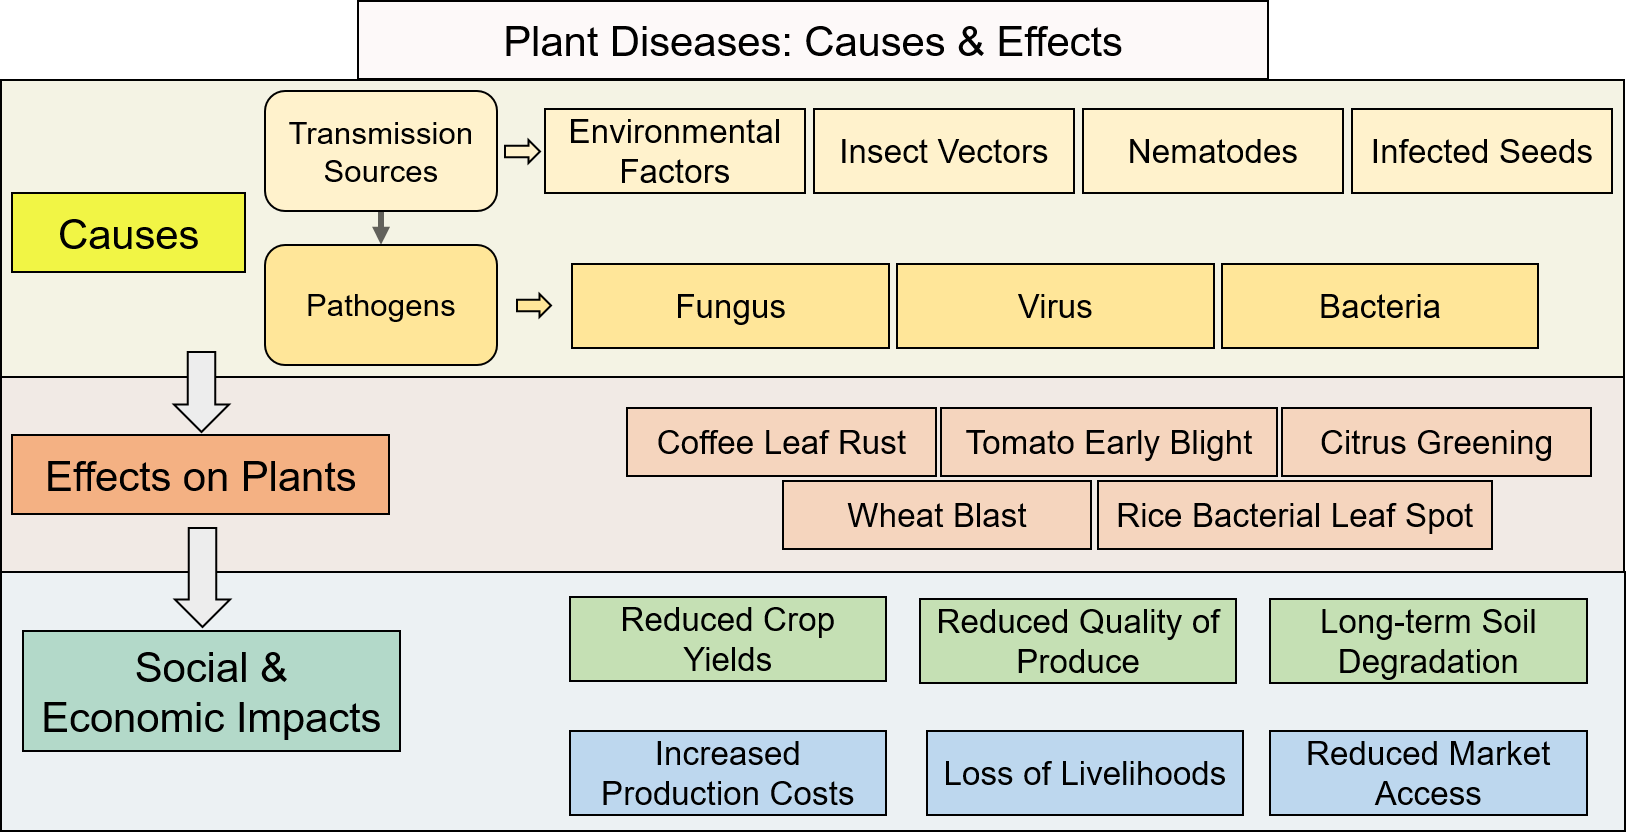
\includegraphics[width=0.85\textwidth]{Figure_1.png}
    \caption{Plant disease causes and effects. This flowchart illustrates the main causes of plant diseases, their effects on plants, and the resulting social and economic impacts.}
    \label{fig:plant diseases}
\end{figure*}
The primary disease agents create detectable patterns that inform detection system design. Biotic factors (fungi, bacteria, and viruses) typically produce signature visual symptoms that RGB imaging can capture: fungi often cause distinctive lesions and color changes \citep{demir2023biological}, while viruses like the Tomato brown rugose fruit virus create textural alterations detectable through advanced image processing \citep{zhang2022tomato}. Hyperspectral imaging provides particular advantages for detecting abiotic stressors (nutrient deficiencies, drought, or chemical damage), which often manifest as subtle spectral changes before visible symptoms appear.

The progression of disease also influences the selection of detection approaches. Early-stage infections, responsible for an estimated 10\% of global food production losses \citep{EconRev}, often exhibit minimal visual symptoms while producing significant spectral alterations detectable through HSI. As infections advance, RGB-based methods become increasingly effective at identifying the morphological and color changes that accompany severe infection. This progression highlights why integrated detection systems that combine multiple imaging modalities offer the most comprehensive disease monitoring capabilities.

The geospatial and temporal dynamics of disease spread further inform detection system design. Diseases like \textit{Xylella fastidiosa} spread in patterns that can be monitored through wide-area surveillance systems \citep{fisher2020threats}, while climate-sensitive pathogens require detection systems capable of functioning under variable environmental conditions \citep{willocquet2020polyetic}. These ecological considerations directly influence the robustness requirements for field-deployed detection technologies.
The flowchart in Figure \ref{fig:plant diseases} illustrates how disease causal factors create specific biological signatures that detection technologies target, ultimately affecting economic and social outcomes. This biological context provides the foundation for the technical approaches discussed in subsequent sections, where RGB and hyperspectral imaging technologies are specifically designed to capture these disease signatures at different development stages and across diverse agricultural environments.

\subsection{Role of Artificial Intelligence in Plant Disease Detection}
Artificial Intelligence (AI), particularly through machine and deep learning, has emerged as a transformative force in plant disease detection. These technologies analyze complex visual patterns in plant imagery to identify diseases with unprecedented speed and accuracy compared to traditional manual inspection methods. Convolutional neural networks (CNNs) have been particularly effective, with reviews demonstrating their high accuracy in classifying various leaf diseases such as blight and powdery mildew.
The practical implementation of these technologies has extended to field-deployable solutions. Mobile applications like Plantix \citep{rani2023role} use image recognition to identify over 60 different plant diseases and provide treatment recommendations, while UAV-mounted systems conduct aerial surveillance to detect disease hotspots across large cultivation areas \citep{sahoo2024transforming}. These applications demonstrate how AI bridges the gap between advanced algorithms and practical agricultural needs. This technological context provides the foundation for our subsequent analysis of detection methodologies, beginning with an examination of the datasets and evaluation metrics that underpin both RGB and hyperspectral imaging approaches to plant disease identification.


\section{Datasets for Plant Disease Detection} \label{sec:evd}
In machine and deep learning, algorithms learn from large datasets to uncover patterns, make predictions, and improve decision-making. These models are trained using datasets, enabling them to identify complex relationships within the data. Labeled examples allow the algorithms to learn from inherent patterns and correlations, enhancing their ability to generalize and accurately predict outcomes on new data. These datasets' quality, quantity, and diversity are crucial, as they promote reliable and robust machine learning models. A well-curated dataset is essential for the model's adaptability to different environments and ability to provide valuable insights. Therefore, the dataset's characteristics significantly impact the model's performance, highlighting the importance of datasets in the effectiveness and transferability of machine and deep learning applications across various fields. This section will explore popular plant disease detection research datasets, summarized in Table \ref{tab:datasets}.




\begin{footnotesize}
\begin{longtable}{@{}p{3cm}p{2cm}p{2cm}p{5cm}@{}}
\caption{Summary of datasets employed in plant disease detection studies, including details on the environment, size, categories, annotations, characteristics, and challenges}\label{tab:datasets} \\

  \toprule
  \textbf{Dataset} & \textbf{Environment} & \textbf{Size} & \textbf{Details} \\
  \midrule
  \endfirsthead

  \toprule
  \textbf{Dataset} & \textbf{Environment} & \textbf{Size} & \textbf{Details} \\
  \midrule
  \endhead

  \midrule
  \multicolumn{4}{r}{{Continued on next page}} \\
  \midrule
  \endfoot

  \bottomrule
  \endlastfoot

  Plant Village \citep{mohanty2016using} & Lab & 54,303 & \textbf{Categories}: 38, \textbf{Annotations}: Labels, \textbf{Characteristics}: Captured in a lab, single leaf per image, uniform background, \textbf{Challenges}: Data imbalance, fine-grained classification \\
  \midrule
  Plant Doc \citep{mohanty2016using} & Natural \& Lab & 2,569 & \textbf{Categories}: 30, \textbf{Annotations}: Labels \& Bounding Boxes, \textbf{Characteristics}: Field images, some misclassification, \textbf{Challenges}: Imbalanced data, variability \\
  \midrule
  Cassava Leaf Disease \citep{Cassava_Competition} & Natural & 21,367 & \textbf{Categories}: 5, \textbf{Annotations}: Labels, \textbf{Characteristics}: Crowd-sourced from farmers, \textbf{Challenges}: Real-world variability \\
  \midrule
  FieldPlant \citep{moupojou2023fieldplant} & Natural & 5,170 & \textbf{Categories}: 27, \textbf{Annotations}: Labels \& Bounding Boxes, \textbf{Characteristics}: Collected from plantations, complex backgrounds, \textbf{Challenges}: Imbalanced data, cluttered environment \\
  \midrule
  CD\&S \citep{CDS} & Natural & 1,597 & \textbf{Categories}: 3, \textbf{Annotations}: Labels \& Bounding Boxes, \textbf{Characteristics}: Field-acquired, augmented images, \textbf{Challenges}: Disease classification \\
  \midrule  
  JMuBEN \citep{jepkoech2021jmuben2} & Natural & 58,555 & \textbf{Categories}: 5, \textbf{Annotations}: Labels, \textbf{Characteristics}: Multiclass classification, \textbf{Challenges}: Small image resolution \\
  \midrule
  Cucumber Disease Dataset \citep{sultana2023dataset} & Natural & 6,400 & \textbf{Categories}: 8, \textbf{Annotations}: Labels, \textbf{Characteristics}: Multiclass classification, augmented images, \textbf{Challenges}: Fine-grained classification \\
  \midrule
  Tobacco Leaf Abnormality \citep{lin2024few} & Natural & 1,430 & \textbf{Categories}: 16, \textbf{Annotations}: Labels, \textbf{Characteristics}: Single disease focus, high resolution images, \textbf{Challenges}: Class imbalance, disease similarity \\
  \midrule
  Tobacco Plant Disease Dataset \citep{tpdd} & Natural & 2,721 & \textbf{Categories}: 12, \textbf{Annotations}: Labels \& Bounding Boxes, \textbf{Characteristics}: Detailed multi-class annotations, \textbf{Challenges}: Occlusion, fragmented disease recognition \\
  \midrule
  BananaLSD \citep{bhuiyan2023bananasqueezenet,arman2023bananalsd} & Natural & 1,600 & \textbf{Categories}: 4, \textbf{Annotations}: Labels, \textbf{Characteristics}: Field-captured smartphone images, expert pathologist labeling, \textbf{Challenges}: Three distinct leaf spot diseases, real-world variability \\
  \midrule
  Banana Leaves Imagery \citep{mduma2025banana} & Natural & 11,767 & \textbf{Categories}: 3, \textbf{Annotations}: Labels, \textbf{Characteristics}: Multi-regional collection, high-resolution smartphone capture, \textbf{Challenges}: Geographic diversity, disease severity variation \\
  \midrule
    Tanzania Banana Leaf Dataset \citep{mduma2022nelson} & Natural & 17,068 & \textbf{Categories}: 3, \textbf{Annotations}: Labels, \textbf{Characteristics}:Farmer garden collection, Camera device standardization, \textbf{Challenges}: Real-world field variability, mobile image quality consistency \\
   \midrule
  PSFD-Musa Banana Leaf Dataset\citep{medhi2022psfd} & Natural & 8,000 & \textbf{Categories}: 15, \textbf{Annotations}: Labels, \textbf{Characteristics}: Multi-aspect banana health assessment, augmented images, \textbf{Challenges}: Multi-class identification, diverse disease types \\
  \midrule
  Makerere AI Bean Disease \citep{makerere2020bean} & Natural & 1,295 & \textbf{Categories}: 3, \textbf{Annotations}: Labels, \textbf{Characteristics}: Smartphone-captured field images, expert annotation by NaCRRI, \textbf{Challenges}: Real-world variability, mobile deployment requirements \\
  \midrule
  CGIAR Bean Disease \citep{gomez2024advancing} & Natural & 9,969 & \textbf{Categories}: 6, \textbf{Annotations}: Labels \& Bounding Boxes (34,053 micro annotations), \textbf{Characteristics}: Multi-disease coverage, both leaf and pod samples, disease hotspot collection, \textbf{Challenges}: Complex backgrounds, co-occurring diseases, large-scale variations \\
  \midrule
  AMG\textsubscript{HS} \citep{Sama_2023_ICCV} & Natural & 6,127 & \textbf{Categories}: 2, \textbf{Annotations}: Labels \& Segmentation, \textbf{Characteristics}: Top-view of crops, segmentation masks, \textbf{Challenges}: Detection and localization of plant stress \\
  \midrule 
  PlantSeg \citep{wei2024plantseg} & Natural & 11,400 & \textbf{Categories}: 115, \textbf{Annotations}: Labels \& Segmentation, \textbf{Characteristics}: In-the-wild images, diverse environments, segmentation masks, \textbf{Challenges}: Disease region identification and classification \\

\end{longtable}
\end{footnotesize}



\subsection{PlantVillage}
The Plant Village dataset contains 54,305 unique leaf images, each 256x256 RGB format pixels across 14 crop types \citep{mohanty2016using}. It spans 38 categories, including species, diseases, and healthy states. The leaves, carefully separated from plants, were photographed against grey and black backgrounds, with the collection featuring both original and grayscale images. The dataset focuses on single leaves against uncluttered backgrounds, limiting its ability to simulate real field conditions and failing to accurately capture the complexities of potential occlusion and clutter found in natural environments. Despite this, PlantVillage remains a significant resource, offering various disease examples across various plant species.

\subsection{PlantDoc}

The PlantDoc dataset comprises 2,598 high-quality images encompassing 27 distinct classes across 13 plant species \citep{singh2019plant}. Curated from Google Images and Ecosia, a meticulous filtering process ensures precision. Reflecting real-world agricultural conditions, this dataset serves as a valuable asset in agricultural computer vision. It provides authentic data crucial for the development of robust plant disease detection algorithms. The authors have introduced the Cropped PlantDoc dataset (C-PD), derived by extracting annotated regions from the original PlantDoc dataset. This process, utilizing bounding box information, aids in eliminating background noise, allowing the model to focus on the essential elements associated with disease symptoms.

\subsection{FieldPlant}
The production value of tomatoes for the processing market in the United States was approximately USD1.16 billion in 2022, highlighting the economic significance of maintaining healthy crops through effective disease management \citep{statista2023tomatoproductionvalue}. Supporting this critical agricultural sector, datasets like FieldPlant, containing 5,170 manually annotated images across 27 disease classes for crops including tomato, corn, and cassava \citep{moupojou2023fieldplant}, enable the development of computer vision algorithms that can detect diseases under realistic farming conditions, potentially safeguarding billions in crop value through appropriate intervention.

\subsection{Cassava Leaf Disease Dataset}
In 2021, Ghana saw its cassava production reach over 22.6 million metric tons, up from 21.77 million metric tons in 2020, continuing a growth trend that started in 2009 \citep{statista2023cassavaproductionghana}. Cassava is a key agricultural crop in Ghana, crucial for staple foods and contributing significantly to the GDP of the agricultural sector. In 2020, Kaggle launched a competition with a dataset of 21,397 cassava plant images, divided into five categories: Cassava Bacterial Blight, Cassava Brown Streak Disease, Cassava Green Mottle, Cassava Mosaic Disease, and Healthy Leaves \citep{Cassava_Competition}. This dataset, taken directly from fields, presents real-world challenges like occlusion and clutter, making it valuable for training models to recognize diseases in complex settings. The class imbalance within the dataset offers a unique opportunity for deep learning models to adapt and overcome this challenge, enhancing their ability to handle real-world data variability.

\subsection{Corn Disease \& Severity Dataset (CD\&S)}
In 2021-2022, corn emerged as the leading grain crop globally, with production surpassing 1.2 billion metric tons, underscoring its vital role in meeting industrial needs \citep{statista2023grainproduction}. The CD\&S dataset, collected at Purdue University's Agronomy Center for Research and Education in West Lafayette, Indiana, comprises unprocessed field imagery under real-world conditions \citep{CDS}. It includes 511, 524, and 562 raw images capturing Northern Leaf Blight, Gray Leaf Spot, and Northern Leaf Spot in maize, with half of the images from each category annotated with bounding boxes. Researchers also acquired an additional 515 raw images of NLS specifically for disease severity analysis. In total, the CD\&S dataset contains 4,455 images, combining 2,112 original field images with 2,343 augmented ones, creating a comprehensive resource for developing accurate corn disease detection algorithms under authentic farming conditions.

\subsection{Arabica Coffee Disease Dataset (JMuBEN)}
Coffee covers one of the largest portions of the hot beverage market. 
Detecting coffee leaf diseases during the early growth stages is crucial for preventing significant yield losses and maintaining production efficiency. JMuBEN dataset provides a valuable resource for training deep learning models to distinguish coffee leaf diseases \citep{jepkoech2021jmuben2}. The dataset contains 58,555 images of Arabica coffee leaves, each with a resolution of 128x128 pixels, spanning five different classes. This extensive collection enables the research into the health and pathology of Arabica coffee plants.

\subsection{Cucumber Disease Recognition Dataset}
Cucumber (Cucumis sativus L.) represents a significant global vegetable crop, with worldwide production reaching 94.7 million tons in 2022 and facing devastating diseases such as downy mildew that can cause yield losses up to 100\% in favorable conditions \citep{abdelfatah2025control}. To address these critical disease management challenges, a comprehensive cucumber disease dataset was created in collaboration with agricultural experts, featuring eight disease classifications. This dataset includes 1280 original field images, which were augmented to 6400 images using various techniques \citep{sultana2023dataset}. These resources are designed to enhance the development of machine vision algorithms to accurately and efficiently diagnose cucumber diseases.

\subsection{Tobacco Leaf Disease Datasets}
Tobacco is an economically viable crop but diseases and pests significantly affect the quality and yield. The Tobacco Leaf Abnormality (TLA) dataset was collected during the crop's mature period in July and August, under field conditions. It includes a total of 1430 images divided into 16 categories: ten infection diseases (bacterial, fungal, and viral), three non-parasitic diseases, two pest traces, and a healthy category \citep{lin2024few}. The dataset, labeled by tobacco agronomists, is valuable for identifying common infections across different tobacco cultivation areas. Tobacco Plant Disease Dataset (TPDD) is another dataset that is used for training deep learning models. It consists of 2721 images divided into 12 classes with annotations for classification and detection \citep{tpdd}.


\subsection{Banana Disease Datasets}
Global banana production reached approximately 135 million tons in 2022, contributing an estimated USD 92.1 billion to the global economy, with worldwide banana exports valued at USD 14.4 billion in 2023 \citep{fao2024banana}. However, Black Sigatoka disease alone causes the greatest yield losses in banana plantations globally, with climate change increasing its risk by 44 percent since the 1970s and potential yield reductions of up to 80 percent \citep{bebber2020climate}. Current research indicates that Black Sigatoka results in an average 3\% reduction in global annual production, representing a loss of yearly revenue of approximately USD 1.6 billion \citep{bebber2020climate}. To address these critical challenges, several comprehensive datasets have been developed for banana disease detection. The BananaLSD dataset comprises 937 original RGB images captured using smartphone cameras in banana fields at Bangabandhu Sheikh Mujibur Rahman Agricultural University, Bangladesh, with an augmented version containing 1,600 images covering Sigatoka, Cordana, Pestalotiopsis, and healthy banana leaves \citep{arman2023bananalsd}. The Tanzania Bananas Dataset contains 17,068 mobile phone-captured images from farmer's gardens using the AdSurv application, comprising 5,883 healthy, 6,147 Black Sigatoka, and 5,038 Fusarium Wilt Race 1 labeled instances collected through Samsung devices for real-world agricultural applications \citep{mduma2022nelson}. The Banana Leaves Imagery dataset provides 11,767 high-resolution images from Tanzania, including 3,339 healthy images, 3,496 Black Sigatoka affected images, and 4,932 Fusarium Wilt Race 1 affected images, collected through collaboration between farmers, researchers, and plant pathologists across multiple districts \citep{mduma2025banana}. Additionally, the PSFD-Musa dataset offers a holistic approach with over 8,000 augmented images covering banana variety classification, disease identification (including Black Sigatoka, Yellow Sigatoka, Panama disease, and others), and nutrient deficiency detection \citep{medhi2022psfd}. These datasets collectively provide comprehensive resources for developing robust machine learning diagnostic tools capable of addressing the significant economic impact of banana diseases on global agricultural systems.

\subsection{Common Beans Disease Datasets}
Common beans (Phaseolus vulgaris) represent the most important legume for direct human consumption globally, with production reaching approximately 27.5 million tons in 2020 and serving as a critical protein source for over 300 million individuals, particularly in Africa and Latin America \citep{kew2021common}. However, bean cultivation faces significant threats from diseases that can drastically reduce yield and quality. Common Bacterial Blight (CBB) causes yield losses ranging from 30 to 70\% in susceptible cultivars globally, while Angular Leaf Spot (ALS) leads to yield losses of 50 to 60\% in Africa \citep{gomez2024advancing}. In Ethiopia alone, CBB can cause 22\% yield reduction in sole cropping systems, while ALS can result in over 47\% yield loss under favorable conditions for disease development \citep{adugna2022evaluation}. To address these critical agricultural challenges, several comprehensive datasets have been developed for automated bean disease detection. The Makerere AI Lab Bean Disease Dataset comprises 1,295 smartphone-captured images collected from real fields across different districts in Uganda in collaboration with the National Crops Resources Research Institute (NaCRRI), covering three classes: healthy beans, Angular Leaf Spot, and Bean Rust \citep{makerere2020bean}. This dataset has been widely adopted in the machine learning community and is available through multiple platforms including TensorFlow Datasets and Hugging Face, with standardized 500x500 pixel RGB images specifically designed for mobile deployment to assist smallholder farmers. Additionally, a more comprehensive multi-disease dataset has been compiled from disease hotspots in Africa and Colombia, encompassing five major bean diseases: Angular Leaf Spot (ALS), Common Bacterial Blight (CBB), Common Bean Mosaic Virus (CBMV), Bean Rust, and Anthracnose, covering both leaf and pod samples under real-field conditions \citep{gomez2024advancing}. These datasets collectively provide essential resources for developing robust machine learning diagnostic tools capable of early disease identification in diverse agricultural environments, ultimately supporting sustainable bean production and food security in regions where beans serve as a primary protein source. 


\subsection{AGricolaModerna Healthy-Stress (AMG\textsubscript{HS})
}
The AMG\textsubscript{HS} Dataset, an extension of the AGM Dataset, has been meticulously assembled to identify and highlight instances of plant stress in images of harvested crops. It contains 6,127 RGB images, each 120x120 pixels, curated from the broader AGM Dataset, which features various plant species. This dataset is categorized into healthy (3,798 images) and stressed (2,329 images) samples, covering 14 out of the 18 classes in the AGM dataset. It includes classification labels to differentiate between healthy and stressed states and segmentation masks pinpointing stressed areas \citep{Sama_2023_ICCV}.

\subsection{PlantSeg}
PlantSeg represents a significant advancement in plant disease detection research, comprising over 11,400 annotated disease images and 8,000 healthy plant images captured across diverse environmental conditions \citep{wei2024plantseg}. The dataset spans 115 distinct plant diseases, with each image featuring precise segmentation masks that identify diseased regions. Unlike existing datasets that primarily contain images from controlled laboratory settings, PlantSeg focuses on in-the-wild plant disease images, enhancing its practical applicability for real-world agricultural scenarios. The dataset distinguishes itself through its comprehensive segmentation annotations, where each image includes detailed masks paired with plant type and disease classifications. This contrasts with conventional datasets that typically offer only basic class labels or bounding box annotations. By capturing the complexity of natural environments and providing high-quality segmentation labels, PlantSeg addresses a critical gap in plant pathology research, enabling the development of more robust and practical disease detection systems for real-world agricultural applications.




\par The existing datasets used for training deep learning models for plant disease detection have several drawbacks. Class imbalance can be one of the hurdles as it can skew the performance of deep learning models towards the majority class, leading to poor generalization \citep{ahmad2021plant}. Several models and strategies are proposed to address class imbalance in plant disease detection. Augmentation techniques can balance the number of images in underrepresented classes and artificially increase the representation \citep{alruwaili2019efficient}. Additionally, the researchers have used loss functions that can enhance the sensitivity of the models toward underrepresented classes \citep{zhong2020research}. Therefore, integrating techniques like class weighting and advanced augmentation strategies can significantly improve the robustness of plant disease detection models against class imbalance. Apart from supervised techniques, unsupervised learning methods can also deal with class imbalance as these models do not rely on labeled data, hence minimizing the effect of skewness \citep{nazki2020unsupervised}. 
Another limitation of current datasets is their tendency to contain images captured in controlled environments, limiting their applicability to real-world field conditions. These datasets often fail to reflect the variation in lighting, background, and plant health statuses, that are common in agricultural settings. As a result, models trained on such datasets may not perform well in real-world scenarios \citep{gong2023analysis}. Furthermore, datasets like PlantDoc have been found to contain misclassified images due to the lack of domain expertise during annotation, which hinders the performance of deep learning models in disease detection \citep{moupojou2023fieldplant}. Finally, the variability in leaf shapes and disease representations complicates the detection process, as many datasets are unstructured or weakly structured, leading to inconsistencies in disease identification \citep{kim2022instance}. This variability, along with inconsistent labeling, poses additional challenges for models trying to generalize across different plant species and disease conditions.


\section{Evaluation Metrics in Plant Disease Detection} \label{sec:em}

The assessment of automated plant disease detection methods relies on standardized evaluation metrics that quantify performance across varying detection tasks. This section examines the principal metrics used to evaluate detection systems and their specific implications for agricultural applications. Detailed mathematical formulations are provided in Table \ref{tab:metrics_summary}.

\subsection{Performance Evaluation Framework}

\subsubsection{Foundational Concepts}
Plant disease detection evaluation centers on four fundamental outcomes: True Positive (TP) - disease correctly identified in infected plants; False Positive (FP) - disease incorrectly identified in healthy plants; False Negative (FN) - disease missed in infected plants; and True Negative (TN) - healthy plants correctly identified. Each outcome carries distinct agricultural implications: false positives trigger unnecessary treatments, increasing costs and potential ecological harm, while false negatives allow diseases to spread unchecked, potentially resulting in significant crop losses.

\subsubsection{Classification Metrics}
Classification metrics evaluate the fundamental task of determining plant health status or identifying specific pathogens. \textbf{Accuracy} provides overall correctness but presents limitations with imbalanced datasets common in agricultural scenarios. \textbf{Precision} measures prediction reliability, becoming crucial when treatments involve significant costs or potential phytotoxicity. \textbf{Recall} quantifies detection completeness, paramount for highly contagious diseases where missing infections could compromise entire fields. \textbf{F1-score} balances precision and recall, providing comprehensive assessment when both treatment costs and missed detection risks must be considered.

\subsubsection{Object Detection Metrics}
Object detection extends classification by simultaneously localizing and identifying multiple disease instances within single images. \textbf{Mean Average Precision (mAP)} evaluates both localization accuracy and classification performance across all disease classes. In agricultural applications, mAP directly correlates with the ability to target interventions precisely, enabling spot treatments that reduce chemical usage and minimize environmental impact while maintaining effective disease control.

\subsubsection{Semantic Segmentation Metrics}
Semantic segmentation performs pixel-level classification to delineate diseased regions from healthy tissue, enabling precise severity quantification. \textbf{Mean Intersection over Union (mIoU)} measures overlap between predicted and ground truth disease regions, while \textbf{Dice Coefficient} offers alternative overlap assessment emphasizing true positives. In plant pathology applications, segmentation scores typically require thresholds above 0.85 to provide sufficient accuracy for disease severity assessment and progression monitoring.

\subsubsection{Regression Metrics for Severity Assessment}
Disease severity quantification requires continuous variable prediction capabilities. \textbf{Coefficient of Determination ($R^2$)} measures the proportion of variance explained by the model in predicting severity levels. Strong $R^2$ values enable detection of physiological responses before visible symptoms appear, providing critical early intervention windows that substantially improve disease management outcomes.

\begin{table*}[h!]
\centering
\small
\caption{Summary of Evaluation Metrics for Plant Disease Detection Applications}
\label{tab:metrics_summary}
\resizebox{\textwidth}{!}{%
\begin{tabular}{@{}p{3cm}p{3.5cm}p{3cm}p{4.5cm}@{}}
\toprule
\textbf{Metric Category} & \textbf{Metric} & \textbf{Formula} & \textbf{Agricultural Application} \\
\midrule
\multirow{4}{*}{\textbf{Classification}} 
& Accuracy & $\frac{TP + TN}{TP + TN + FP + FN}$ & Overall performance assessment \\
\cmidrule(lr){2-4}
& Precision & $\frac{TP}{TP + FP}$ & Minimizing unnecessary treatments \\
\cmidrule(lr){2-4}
& Recall (Sensitivity) & $\frac{TP}{TP + FN}$ & Critical for contagious diseases \\
\cmidrule(lr){2-4}
& F1-score & $2 \times \frac{\text{Precision} \times \text{Recall}}{\text{Precision} + \text{Recall}}$ & Balanced assessment \\
\midrule
\textbf{Object Detection} & Mean Average Precision (mAP) & $\frac{1}{N} \sum_{i=1}^{N} \int_{0}^{1} p(r) \, dr$ & Targeted intervention planning \\
\midrule
\multirow{2}{*}{\textbf{Segmentation}} 
& Mean IoU (mIoU) & $\frac{TP}{TP + FP + FN}$ & Severity quantification \\
\cmidrule(lr){2-4}
& Dice Coefficient & $\frac{2 \times TP}{2 \times TP + FP + FN}$ & Boundary delineation accuracy \\
\midrule
\textbf{Regression} & R-squared ($R^2$) & $1 - \frac{\sum_{i=1}^{n} (y_i - \hat{y}_i)^2}{\sum_{i=1}^{n} (y_i - \bar{y})^2}$ & Early detection capability \\
\bottomrule
\end{tabular}%
}
\end{table*}

\subsection{Metric Selection for Plant Disease Detection Applications}

Appropriate metric selection must align with specific agricultural objectives and disease characteristics. For rapidly spreading diseases like late blight, recall optimization minimizes missed infections that could cause field-wide devastation. Precision-focused systems reduce unnecessary chemical applications, potentially decreasing fungicide usage by up to 35\% with variable-rate technology sprayers \citep{tona2018profitability}. Crop value influences metric prioritization: high-value specialty crops may justify recall-optimized systems despite higher false positive rates, while commodity crops typically require precision optimization for economic viability. These metrics, combined with specialized datasets, establish the foundation for developing robust plant disease detection algorithms across diverse agricultural environments.



\section{Color Imagery-Based Approaches for Disease Detection}\label{sec:dlc}
Traditional methods of plant disease detection using color or RGB imagery have been primarily based on image processing techniques that focus on color analysis, segmentation, and feature extraction. A fundamental approach involves analyzing chromatic variations in plant tissues to identify disease symptoms, including discoloration and the presence of lesions. Color thresholding techniques have been employed to segment affected areas from healthy regions, enabling quantitative assessment of disease severity through measurement of the proportion of diseased pixels \citep{beron2020detection}.


\begin{figure}[h!]
\centering
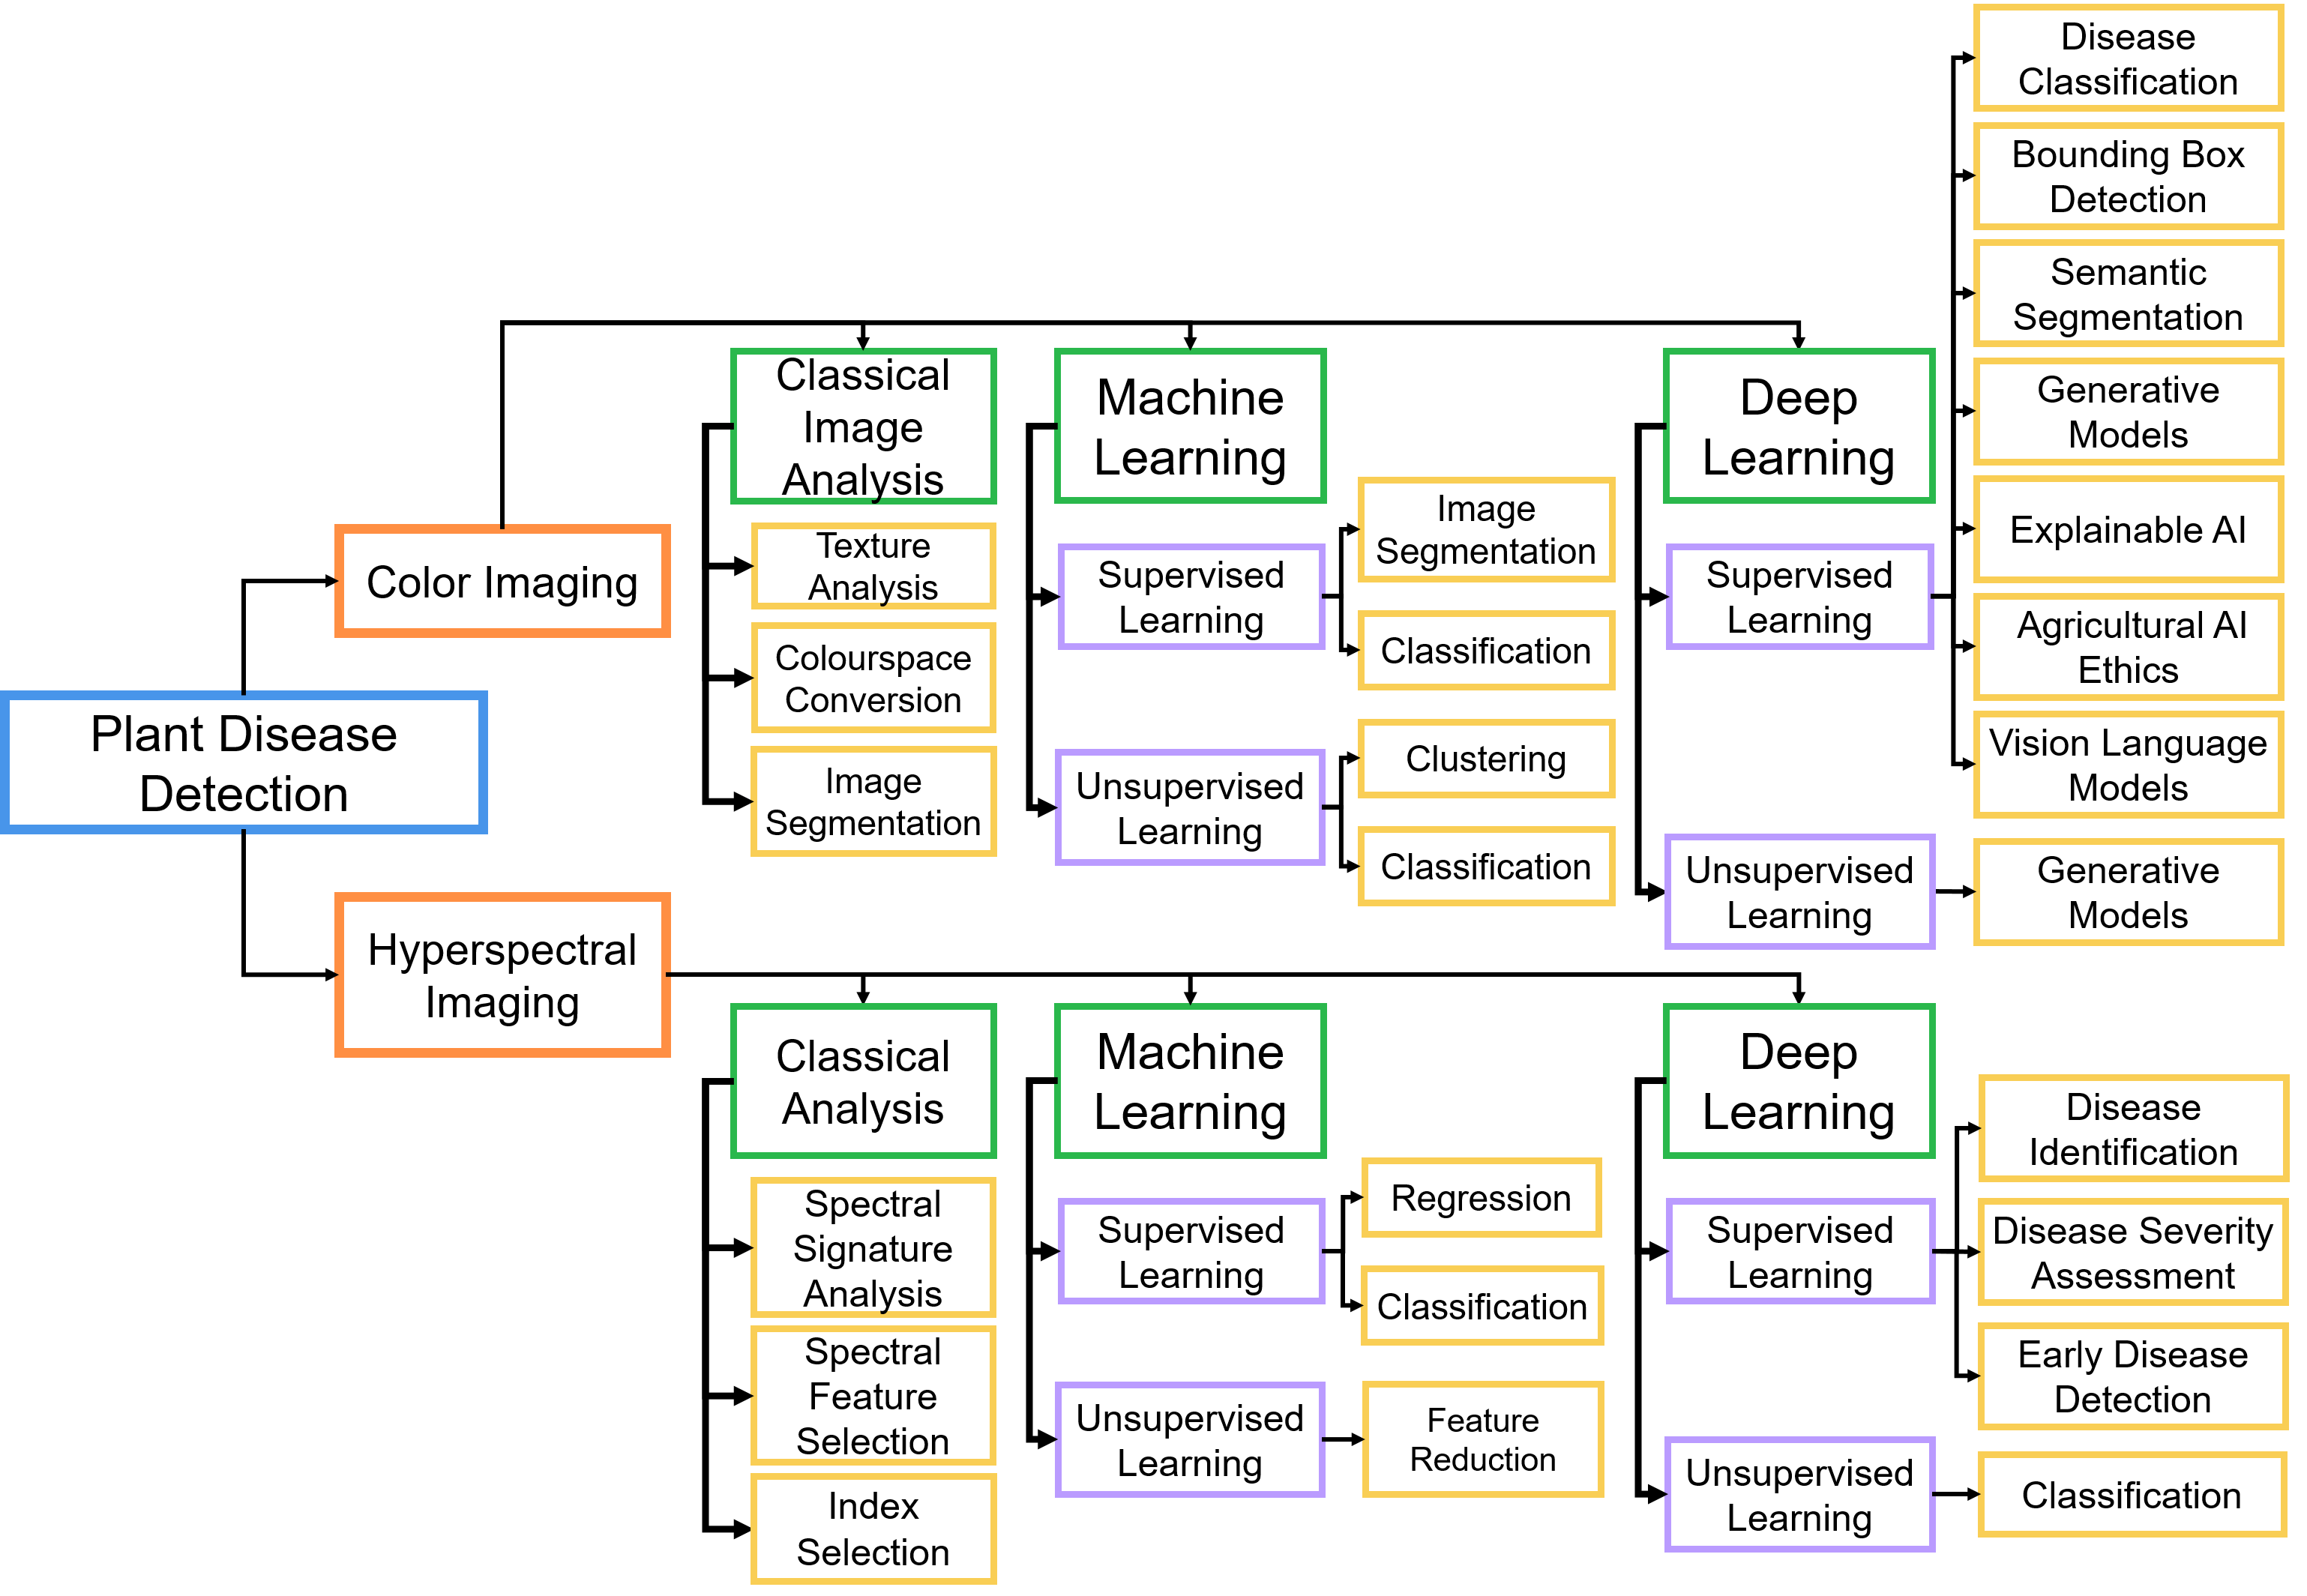
\includegraphics[width=1\textwidth]{Figure_2.png}
\caption{Comprehensive taxonomy of existing literature on plant disease detection using color and hyperspectral imaging modalities. The hierarchical structure categorizes detection methodologies into three fundamental approaches: classical image processing, machine learning techniques, and deep learning frameworks, demonstrating the evolutionary trajectory from conventional analytical methods to advanced computational learning paradigms.}
\label{fig:taxonomy}
\end{figure}


Additional methods such as edge detection and image enhancement have been utilized to improve the visibility of disease symptoms. Algorithms based on principal component analysis have been developed to enhance color contrast and facilitate improved feature extraction from RGB imagery \citep{palanivel2017pca}. Genetic algorithms have been applied to optimize the detection of diseased regions in plant tissues by analyzing color variations indicative of pathological conditions \citep{singh2015detection}.
Contemporary approaches have transitioned toward deep learning techniques, particularly Convolutional Neural Networks (CNNs), which automate the feature extraction process and enhance classification accuracy across multiple disease categories \citep{mohanty2016using}. These methods utilize large datasets and demonstrate improved generalization to diverse field conditions, addressing the limitations of traditional techniques that often exhibit reduced performance under variable environmental factors \citep{sladojevic2016deep}. The integration of machine learning with traditional image processing has resulted in hybrid models that enhance detection capabilities by combining the advantages of both methodological approaches \citep{tete2017plant}.
Figure \ref{fig:taxonomy} presents a comprehensive analysis of the current literature on plant disease detection using RGB imagery and hyperspectral imaging. The diagram categorizes plant disease detection methodologies into three primary groups: Classical Analysis, machine learning, and deep learning. The taxonomy illustrates the methodological progression from fundamental techniques to advanced learning-based algorithms.


Table \ref{tab:comparison} presents a comparative analysis of classical methods, machine learning, and deep learning approaches, highlighting their respective strengths and limitations. Classical methods, including logistic regression, demonstrate effectiveness when applied to smaller datasets with manually extracted features, such as disease symptoms or environmental parameters. Machine learning models, including Support Vector Machines (SVM) and Random Forests (RF), are more suitable for handling larger datasets and can partially automate feature selection, thereby improving disease detection accuracy. Deep learning approaches, particularly CNNs and Vision Transformers (ViT), excel in analyzing large, complex image datasets through automated feature extraction, making them highly effective for plant disease detection applications. However, deep learning models require substantial computational resources and often exhibit reduced interpretability compared to classical or machine learning models. The literature on plant disease detection can be systematically categorized into three methodological approaches: classical methods, machine learning, and deep learning, each representing progressive advancements in the field.


\begin{table*}[h!]
\caption{Comparative Analysis of Classical Methods, Machine Learning, and Deep Learning for Plant Disease Detection}
\centering
\small
\label{tab:comparison}
\begin{tabular}{p{2.2cm}>{\raggedright}p{3.2cm}>{\raggedright}p{3.2cm}>{\raggedright}p{3.2cm}}
\hline
\textbf{Feature} & \textbf{Classical Methods} & \textbf{Machine Learning} & \textbf{Deep Learning} \\ 
\hline\hline
Definition & Traditional statistical techniques & Pattern recognition algorithms that learn from training data & Neural network architectures using multiple hidden layers \\ 
\hline
Examples & \raggedright Linear regression, Logistic regression & \raggedright SVM, Random Forests, K-NN & \raggedright CNNs, RNNs, Vision Transformers \\ 
\hline
Data Requirement & Effective with smaller datasets & Handles larger datasets well & Requires extensive datasets \\ 
\hline
Feature Engineering & Extensive manual extraction & Partial automation & Automatic extraction \\ 
\hline
Interpretability & Highly interpretable & Variable interpretability & Limited interpretability \\ 
\hline
Training & Fast training & Requires validation & Computationally intensive \\ 
\hline
Complexity & Simple models & Intermediate complexity & High complexity \\ 
\hline
\end{tabular}
\end{table*}

\subsection{Visual Pattern Analysis: Classical RGB Processing Methods}
Traditional plant disease detection, often dependent on expert visual assessment, faces challenges including subjectivity, difficulty in early symptom identification, vulnerability to human error, high resource demands, reliance on expert availability, and inefficiency for real-time monitoring \citep{wang2017automatic, sankaran2010review}. To overcome these limitations and improve accuracy and efficiency, the adoption of sensors and imaging technologies, alongside detection using machine learning, is crucial. These advancements enable early identification and treatment of diseases, enhancing disease management \citep{gavhale2014overview}. 


\subsubsection{Texture-Based Techniques for Disease Identification}

Texture analysis methodologies for plant disease detection have received considerable attention due to their effectiveness in identifying and classifying diseases based on the visual characteristics of plant foliage. These approaches utilize various image processing techniques to extract texture features that serve as indicators of disease presence. The Gray-Level Co-Occurrence Matrix (GLCM) represents a fundamental technique in texture analysis, quantifying spatial relationships between pixels within an image. This method enables extraction of statistical measures including contrast, correlation, and homogeneity, which function as robust indicators of disease presence \citep{waldchen2018plant}.

Gabor filters and Local Binary Patterns (LBP) are extensively employed for texture feature extraction, providing mechanisms to capture frequency and orientation information from leaf imagery \citep{waldchen2018plant, naresh2016classification}. These methodologies have demonstrated promising results in enhancing the accuracy of disease classification models. Color Coherence Vector (CCV) represents an additional approach that characterizes color distribution within images, facilitating identification of specific regions affected by disease. \citet{abdu2020automatic} implemented CCV and LBP for feature extraction, utilizing a method that encodes texture information based on local pixel intensity patterns surrounding a central pixel, specifically targeting chlorotic and necrotic areas of plant leaves to detect diseases and assess their severity.

\citet{arivazhagan2013detection} developed a methodology incorporating color transformation, green pixel removal, segmentation, and texture statistics, achieving 94\% accuracy in disease classification. Integration of texture features with additional characteristics, including color and shape attributes, enhances the robustness of disease detection systems. \citet{RahayuF2021LeafDC} demonstrated that combining GLCM-derived texture features with color features can achieve classification accuracies exceeding 97\%. Implementation of Principal Component Analysis (PCA) for dimensionality reduction further optimizes feature selection, enabling more efficient model training and improved classification performance \citep{mengistu2018automatic}. Recent developments in machine learning and deep learning have facilitated the creation of more sophisticated models for plant disease detection. Techniques including Support Vector Machines (SVM) and Convolutional Neural Networks (CNN) have been employed to classify diseases based on extracted texture features, achieving high accuracy rates \citep{wu2022research}. \citet{ahmad2021leaf} utilized SVM for disease classification in grapevines, reporting 98.79\% accuracy when combining color and texture features.



\begin{figure*}[h!]
    \centering
    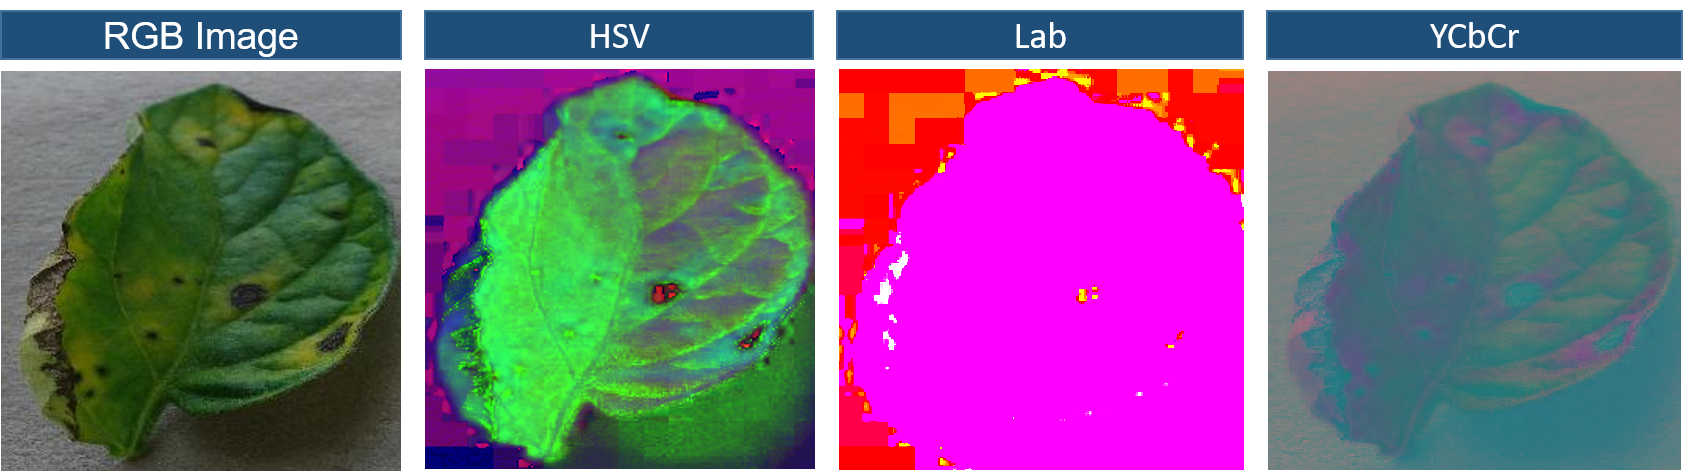
\includegraphics[width=0.95\textwidth]{Figure_4.png}
    \caption{Visualizing plant leaf in multiple color spaces for disease detection: RGB, HSV, LAB and YCbCr representations}
    \label{fig:colorspaces}
\end{figure*}




\subsubsection{Color Space Conversion for Improved Plant Disease Detection}

Color space conversion in image processing involves the transformation of an image from one color model to another, facilitating enhanced analysis capabilities. Different color spaces emphasize distinct aspects of color information that may be less prominent in the original representation. The RGB color space, based on red, green, and blue components, is conventionally utilized for display purposes but may not adequately highlight subtle color variations required for plant disease detection. Converting images to alternative color spaces such as HSV (Hue, Saturation, Value), LAB (Luminance and Color-opponent), or YCbCr (Luminance, Blue-difference, Red-difference) enhances different image characteristics including brightness and color separation, thereby reducing noise and improving the clarity of specific features. Figure \ref{fig:colorspaces} illustrates the visual differences among various color spaces.

Researchers have implemented color space conversions to identify plant diseases through optimized feature extraction. \citet{camargo2009image} developed a technique for identifying banana leaf diseases by converting RGB images into customized color transformations (H, I3a, I3b), specifically optimized for plant disease detection applications. This methodology involves refining segmented images through pixel neighborhood analysis and gradient changes to eliminate irrelevant pixels. \citet{orillo2014rice} implemented a method for classifying rice plant health using image processing combined with back-propagation neural networks, extracting six features from images processed in HSV and LAB color spaces. This approach incorporates color transformation and image enhancement techniques including noise reduction and contrast adjustment. \citet{dhaygude2013agricultural} investigated textural properties using Spatial Gray Dependence Matrix (SGDM) and applied the Hue Saturation Value (HSV) color space to analyze color components in RGB images.


\subsubsection{Threshold-Based Segmentation Methods}

Image segmentation represents a fundamental technique in computer vision that involves partitioning an image into distinct regions for subsequent analysis and classification. This approach enhances the understanding of plant diseases by enabling the isolation and characterization of specific image regions. \citet{patil2011leaf} investigated various thresholding methodologies for pixel classification within image segments. They examined simple thresholding, which employs a single intensity value to separate segments, and triangular thresholding for segmenting leaf areas and lesions to calculate the area quotient, defined as the ratio of lesion area to total leaf area. Triangular thresholding is an image segmentation technique that analyzes pixel intensity histograms to identify triangular distributions representing foreground and background pixels, enabling determination of optimal thresholds that effectively separate objects of interest from background by maximizing contrast and minimizing pixel intensity distribution overlap.

Their investigation also examined advanced analytical techniques including moment analysis for measuring shape properties to facilitate classification, chain code representation for boundary description using directional sequences, bounding box approaches that enclose segmented areas within rectangular regions to simplify analysis, and Scale-Invariant Feature Transform (SIFT) for detecting and describing local image features across different scales for object recognition applications.

\citet{al2013empirical} focused on diagnosing olive leaf spot disease using multiple methodologies including auto-cropping for automatic region of interest extraction, fuzzy c-means classification as a clustering technique where pixels can belong to multiple groups with varying membership degrees, and image enhancement techniques such as median filtering for noise reduction and conversion to LAB color space. They evaluated the comparative effectiveness of fuzzy c-means versus k-means clustering for disease categorization.



\subsection{Feature-Driven Approaches: Machine Learning on RGB Data}

Supervised learning methodologies train models on labeled datasets, developing pattern recognition capabilities and establishing relationships between input features and target outputs, which enables accurate predictions on new data. This approach is particularly suitable for classification and regression tasks in agricultural applications \citep{kotsiantis2007supervised}. Conversely, unsupervised learning operates on unlabeled data to identify underlying structures or patterns, employing techniques such as clustering to group similar data points and dimensionality reduction to streamline data while preserving essential features \citep{usama2019unsupervised}. This methodology is valuable for exploring inherent structures or relationships within data without predefined target outputs. Both supervised and unsupervised learning paradigms are instrumental in enhancing machine learning utility, providing versatile analytical tools for various applications, including plant disease detection in RGB imagery.

\subsubsection{Machine Learning for Plant Disease Classification}

Machine learning approaches for plant disease classification involve categorizing images into predefined classes to identify specific diseases. \citet{qin2016identification} developed classification models for four alfalfa leaf diseases, implementing optimal lesion segmentation methods to distinguish diseased regions from healthy areas. From 1,651 lesion images, 129 attributes related to texture, color, and shape characteristics were extracted, with the most significant features identified through three selection methodologies. The study evaluated Random Forest (RF), Support Vector Machine (SVM), and K-Nearest Neighbors (KNN) algorithms, determining that SVM with 45 ReliefF features achieved 94.74\% accuracy on the test dataset. A Naive Bayes-based semi-supervised model also achieved 80\% accuracy. \citet{kulkarni2012applying} implemented Gabor filters for feature extraction, utilizing Artificial Neural Networks (ANN) to classify plant leaves as healthy or diseased, demonstrating the effectiveness of machine learning in plant disease detection applications.

Recent advances in machine learning for plant disease detection have demonstrated significant improvements in classification accuracy and computational efficiency. \citet{lin2019deep} proposed a semantic segmentation model using Convolutional Neural Networks (CNNs) to recognize and segment powdery mildew in cucumber leaves at the pixel level, achieving an average pixel accuracy of 97.12\%, a joint intersection ratio score of 79.54\%, and a dice accuracy of 81.54\%. The model outperformed established segmentation techniques including Gaussian mixture models, Random Forests, and fuzzy c-means clustering. 

\citet{prince2024csxai} introduced a lightweight CNN-SVM hybrid model (CSXAI) for crop disease detection and classification, incorporating explainable AI visualization through Gradient-weighted Class Activation Mapping (Grad-CAM). Their approach demonstrated superior performance compared to traditional transfer learning models while maintaining computational efficiency suitable for field deployment.

The integration of ensemble methods has shown promising results in improving classification robustness. \citet{hatuwal2020plant} conducted a comparative analysis of machine learning models including SVM, KNN, Random Forest, and CNN for plant leaf disease recognition, with CNN achieving the highest accuracy of 97.89\%, followed by Random Forest at 87.436\%, SVM at 78.61\%, and KNN at 76.969\%. Their work highlighted the importance of feature selection and the effectiveness of ensemble approaches in handling complex disease classification tasks.

Contemporary research has also focused on addressing computational efficiency for practical deployment. \citet{mahmud2024light} developed a streamlined version of the DenseNet architecture specifically for mango leaf disease classification, creating a lightweight model that reduces computational complexity while maintaining high accuracy, making it suitable for resource-limited environments such as mobile devices and edge computing systems commonly used in agricultural applications.



\subsubsection{Machine Learning for Enhanced Image Segmentation}

Machine learning-based image segmentation has substantially advanced digital image analysis capabilities in agricultural applications through the partitioning of images into semantically meaningful regions. In contrast to traditional segmentation techniques, machine learning methodologies can autonomously learn patterns and relationships from training data, facilitating more precise and automated identification of disease-affected areas. \citet{vetal2017tomato} achieved 93.75\% accuracy in tomato plant disease detection using a multiclass Support Vector Machine (SVM) approach. \citet{zhang2019plant} developed a hybrid clustering methodology that combines superpixel segmentation with the expectation-maximization algorithm, which effectively enhanced lesion segmentation performance and demonstrated superior results compared to conventional clustering methods. Similarly, \citet{singh2019plant} implemented an automated detection system employing image analysis and machine learning techniques, achieving a high classification accuracy of 97.6\%.


\subsubsection{Principal Component Analysis and Feature Space Optimization}

Dimensionality reduction techniques, particularly Principal Component Analysis (PCA), facilitate the compression of high-dimensional image data into more computationally manageable representations while preserving essential disease-related features. This approach not only accelerates computational processing but also reduces noise interference in machine learning models, thereby improving detection accuracy. PCA represents a prominent methodology that reduces dataset dimensionality through the selection of variance-maximizing linear combinations of original features. This approach is complemented by alternative methods including Uniform Manifold Approximation and Projection (UMAP) and Linear Discriminant Analysis (LDA), which demonstrate particular effectiveness in handling non-linear data structures.

\citet{wang2012image} demonstrated the application of PCA in automated plant disease diagnosis, emphasizing its role in enhancing backpropagation algorithm performance for diseases including grape downy mildew and wheat leaf rust. Through the integration of advanced image processing techniques with dimensionality reduction methodologies, their investigation demonstrated improved accuracy and computational efficiency in plant disease diagnosis, illustrating the synergy between image analysis techniques and dimensionality reduction strategies.

\subsubsection{Unsupervised Learning Methods for Disease Pattern Recognition}

Clustering represents an unsupervised learning methodology that groups similar disease patterns, proving particularly valuable when labeled training data is limited or unavailable. Techniques including K-means clustering and Self-Organizing Maps (SOMs) facilitate the distinction between healthy and diseased tissue clusters, enabling initial identification prior to more sophisticated analytical procedures.

\citet{alhiary2011fast} and \citet{bagde2015artificial} implemented K-means clustering combined with neural networks for disease recognition and classification, demonstrating the effectiveness of machine learning methodologies in distinguishing between healthy and diseased plant tissues. Self-organizing maps, as employed by \citet{meunkaewjinda2008grape}, provide an unsupervised clustering approach with visualization capabilities applied to grape leaf color detection and disease segmentation. \citet{jaware2012crop} developed a disease detection methodology through image segmentation, transforming RGB leaf images into alternative color spaces and applying K-means clustering for color cluster identification.



\subsection{End-to-End Recognition: Deep Learning for RGB Disease Detection}

Deep learning employs multi-layered neural networks to process complex datasets, enabling automated learning of intricate patterns without manual feature engineering. Convolutional Neural Networks (CNNs) demonstrate particular effectiveness for image analysis through hierarchical feature extraction that captures spatial relationships among pixels. Vision Transformers (ViTs) have emerged as an alternative approach, treating images as sequences of patches and utilizing self-attention mechanisms to capture global context more effectively than traditional local feature extraction methods. The progression of deep learning has facilitated the development of Vision-Language Models (VLMs) \citep{radford2021learning}, which integrate visual and textual information for cross-modal understanding applications including image captioning and visual question answering.

\begin{figure*}[h!]
    \centering
    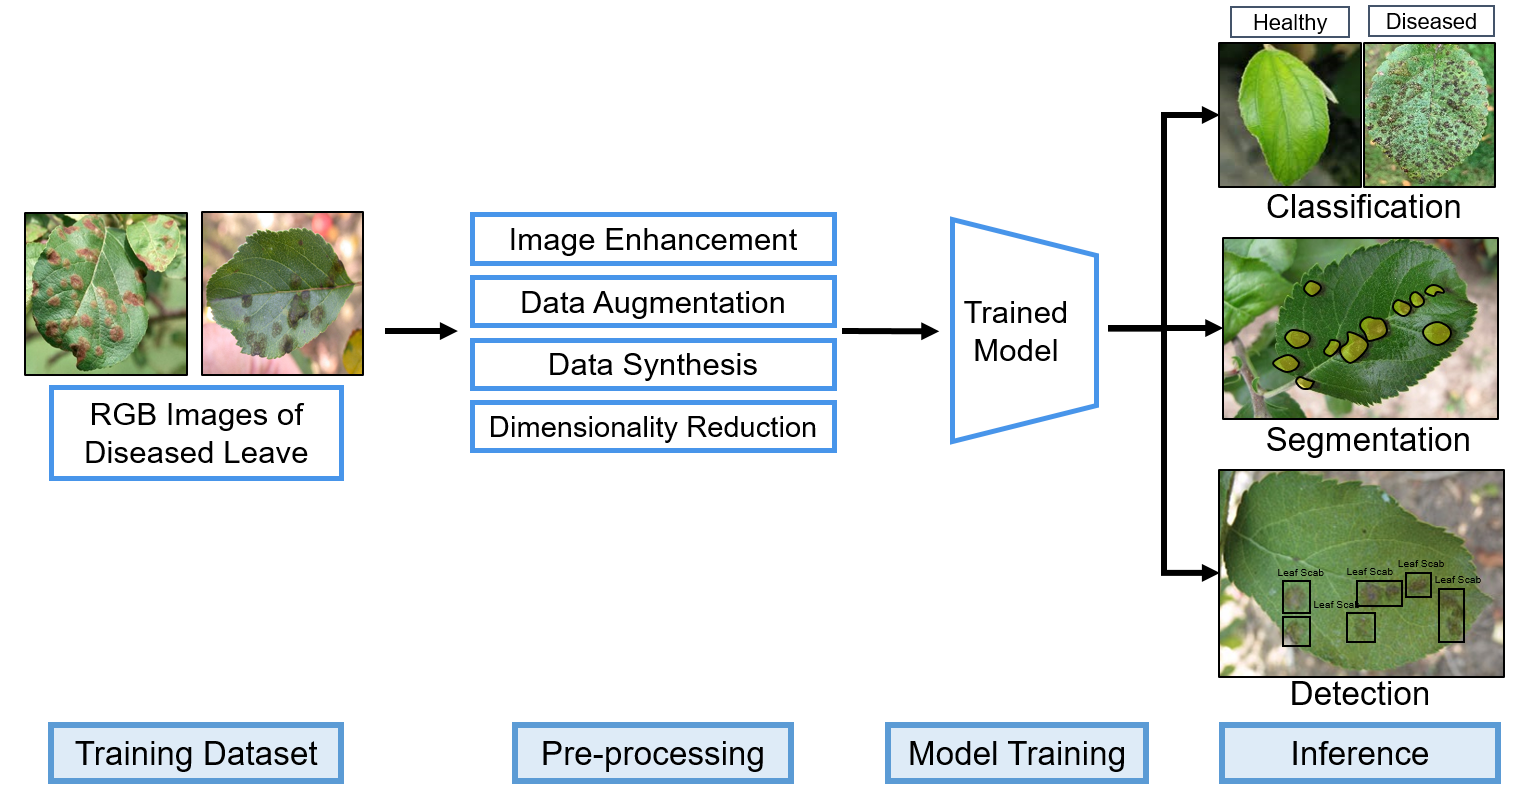
\includegraphics[width=0.85\textwidth]{Figure_5.png}
    \caption{Machine learning pipeline for plant disease detection using RGB images, encompassing pre-processing, model training, and inference to distinguish between healthy and diseased leaves}
    \label{fig:RGB_pipeline}
\end{figure*}

The primary advantage of deep learning lies in automated feature extraction, replacing traditional handcrafted feature methods. CNNs utilize convolutional layers to detect visual patterns at multiple scales, while attention-based models assign varying importance levels to different data elements. This adaptability enables effective scaling with increasing dataset sizes and accommodation of diverse data types. In agricultural applications, deep learning techniques have substantially improved plant disease classification through more accurate and automated diagnosis capabilities. Figure \ref{fig:RGB_pipeline} illustrates the typical workflow of a plant disease detection system, encompassing stages from image acquisition to final classification.


 
\subsubsection{Deep Learning Models for Agricultural Disease Classification}

Deep learning algorithms for plant disease classification analyze visual symptoms on plant tissues to distinguish among various pathological conditions through automated feature extraction and pattern recognition.

\textbf{Species-Specific Neural Network Architectures}
Crop-specific detection strategies have emerged to address distinct disease manifestations across different plant species. \citet{chen2022dfcanet} developed DFCANet for corn leaf disease recognition, achieving 98.47\% accuracy and demonstrating superior performance compared to conventional CNN architectures. \citet{zeng2022lightweight} introduced LDSNet, a lightweight model incorporating attention mechanisms that achieved 95.4\% accuracy for corn disease detection. For olive crops, \citet{lachgar2022optimization} reported 98.43\% accuracy using optimized CNN topologies, while \citet{lin2022few} explored few-shot learning techniques for scenarios with limited training data. \citet{divya_cassava} developed a semi-supervised segmentation-driven classification framework using modified Color Index Vegetation Extraction (CIVE-SSL) to generate pixel-level pseudo labels for cassava leaf disease identification, achieving 89.73\% accuracy while reducing dependence on densely annotated training data for cassava diseases.
Tomato disease detection has received substantial attention, with \citet{sahu2023classification} combining convolutional architectures with traditional machine learning methods to achieve 96\% accuracy. \citet{wu2021multi} implemented vision transformer-based approaches that surpassed standard CNNs with 88.1\% accuracy. \citet{zarboubi2025custombottleneck} developed CustomBottleneck-VGGNet for tomato leaf disease identification, achieving 99.12\% accuracy with only 1.4 million parameters and demonstrating superior performance compared to MobileNetV2, ResNet50, GoogleNet, VGG16, and VGG19 across multiple evaluation metrics. The architectural design incorporating both CBR (Convolution-BatchNorm-ReLU) and CBS (Convolution-BatchNorm-SiLU) blocks demonstrates thoughtful consideration of activation functions, with SiLU implementation in final layers aimed at preserving gradient flow and maintaining nuanced feature representations. \citet{khan2023tomato} proposed a novel convolutional transformer architecture for tomato maturity classification that achieves state-of-the-art performance with 58-66\% improvements in mean average precision across three datasets, including their newly introduced KUTomaData dataset containing 700 greenhouse images from the UAE. \citet{upadhyay2024detecting} developed a modified ResNeXt approach for detecting fungal diseases across multi-crop heterogeneous region datasets (apple, custard apple, and guava), achieving 98.92\% accuracy on 14,408 images, while \citet{upadhyay2024diagnosis} refined the ResNeXt architecture specifically for apple crops through reduced kernel size and grouped convolutions, achieving 98.94\% accuracy. Coffee crop applications demonstrated exceptional performance, with \citet{sharma2023coffee} and \citet{aufar2023web} employing transfer learning on the JMuBEN dataset to achieve near perfect test accuracy using MobileNet and DenseNet architectures, respectively. 

Banana disease detection has demonstrated significant advancement through specialized architectures targeting tropical crop challenges. \citet{selvaraj2019ai} created a robust CGIAR network dataset containing 12,600 field-collected banana images across 18 disease and pest classes, implementing deep transfer learning with three CNN architectures (ResNet50, InceptionV2, MobileNetV1) and achieving over 90\% detection accuracy through expert annotation involving 30,952 labeled samples, demonstrating the effectiveness of heterogeneous field backgrounds for model generalization in real-world agricultural applications. \citet{bhuiyan2023bananasqueezenet} introduced BananaSqueezeNet, a computationally efficient convolutional neural network specifically designed for real-time banana disease identification, achieving comprehensive performance metrics of 96.25\% accuracy, 96.53\% precision, 96.25\% recall, and 95.13\% MCC for three leaf spot diseases while outperforming conventional deep learning architectures and demonstrating multi-disease detection capabilities across leaves, fruits, and stems including black sigatoka, panama disease, and bacterial soft rot with 95.13\% accuracy. \citet{rajalakshmi2025early} developed a specialized deep convolutional neural network for comprehensive banana leaf disease and pest detection, achieving 99\% accuracy through novel architectural design that surpassed comparative deep learning methods and facilitated early-stage intervention strategies for sustainable farming practices in tropical and subtropical regions. \citet{elinisa2024mobile} implemented a mobile-deployed CNN architecture for banana disease identification, achieving 91.17\% accuracy with real-time processing capabilities that deliver classification results with over 90\% confidence in under five seconds per image, demonstrating practical field deployment for Fusarium Wilt and Black Sigatoka detection. \citet{jimenez2025detection} applied CRISP-DM methodology, a systematic six-phase data mining framework encompassing business understanding through deployment, with three pre-trained architectures (EfficientNetB0, ResNet50, and VGG19) for Black Sigatoka and Cordana detection in Ecuadorian banana crops, achieving accuracies of 88.33\%, 88.90\%, and 87.22\% respectively on a dataset of 900 field-collected images expanded to 9,000 through TensorFlow Keras data augmentation techniques.\citet{sujatha2025advancing} proposed an integrated AI solution combining deep learning feature extraction through VGG19 and Inception v3 architectures with machine learning classifiers (SVM, kNN), achieving notable performance variations across species with banana leaf datasets reaching 91.9\% accuracy (Inception v3+SVM) and custard apple datasets achieving 99.1\% accuracy (VGG19+kNN), demonstrating the effectiveness of hybrid DL-ML approaches for multi-species plant disease detection. \citet{thiagarajan2024analysis} addressed CNN limitations in rotation and scale invariance for banana disease detection by proposing two hybrid approaches: ANN integrated with Scale-Invariant Feature Transform (SIFT) for complex pattern recognition through activation function processing, and ANN combined with Histogram of Oriented Gradients (HOG) and Local Binary Patterns (LBP) for local pattern and gradient representation, demonstrating enhanced feature extraction capabilities compared to conventional CNN architectures.




\textbf{Generalized Multi-Species Classification Models}

Universal deep learning models capable of identifying diseases across multiple plant species have demonstrated significant advancement over traditional approaches. \citet{ferentinos2018deep} achieved 99.48\% accuracy using a modified VGG model on the PlantVillage dataset. \citet{wang2021few} developed ITC-Net, integrating image and textual information for disease recognition with 99.66\% accuracy. \citet{zhang2023ibsa_net} proposed IBSA-Net for complex environmental conditions, achieving an F1-score of 0.9433. \citet{yu2023inception} introduced the Inception Convolutional Vision Transformer (ICVT), demonstrating 99.94\% accuracy on PlantVillage and 77.54\% on PlantDoc datasets.

\textbf{Network Architecture Enhancement Strategies}

Architectural optimization techniques have focused on improving computational efficiency while maintaining classification performance. \citet{chen2020identification} developed the Both-channel Residual Attention Network (B-ARNet), achieving 89\% accuracy in tomato disease classification. \citet{atila2021plant} demonstrated EfficientNet's superiority with 99.97\% accuracy on PlantVillage with minimal preprocessing requirements. \citet{hassan2021identification} improved computational efficiency through depth-separable convolutions, achieving 99.56\% accuracy. \citet{ruth2022meta} introduced a two-level weight optimization process combining butterfly optimization and genetic algorithms, reaching 99\% accuracy on modified PlantVillage datasets.


\subsubsection{Object Detection Networks for Spatial Disease Localization}

Object detection methodologies utilizing architectures such as YOLO and Mask R-CNN provide both classification and spatial localization capabilities, enabling precise identification of disease regions within plant tissues. This spatial information facilitates targeted treatment applications, contributing to more effective disease management strategies.

Deep learning-based localization techniques have demonstrated substantial advancement in automated disease region identification. YOLO-based implementations have shown particular effectiveness across diverse crop species. \citet{li2022improved} enhanced YOLOv5s with CSP modules and Transformer encoders, achieving 93.1\% mAP on curated datasets. \citet{qi2022improved} developed SE-YOLOv5 for tomato virus detection, obtaining 91.07\% accuracy with 94.89\% mAP. \citet{li2022yolo} introduced YOLO-JD for jute disease identification, surpassing comparative methods with 96.63\% average mAP.

Crop-specific optimizations have demonstrated enhanced performance for particular species. \citet{zhang2022deep} improved grape downy mildew detection using YOLOv5-CA, achieving 89.55\% mAP, while \citet{xie2020deep} developed Faster DR-IACNN for grape leaf diseases with 81.1\% mAP. Apple disease detection applications include \citet{li2023real} proposing BTC-YOLOv5s with 84.3\% mAP and \citet{liu2022improved} presenting YOLOX-ASSANano achieving 91.08\% mAP on proprietary datasets. \citet{bellout2024advanced} evaluated advanced YOLO models (YOLOv5, YOLOX, YOLOv7, YOLOv8, and YOLO-NAS) for real-time tomato leaf disease detection, with YOLOv5 achieving the highest mean average precision of 93.1\% after hyperparameter optimization on combined PlantDoc and PlantVillage datasets. \citet{zarboubi2023advancing} developed an integrated IoT-based pest management system utilizing YOLOv8m deployed on Raspberry Pi 4B for automated counting of tomato pests in pheromone traps with Firebase cloud integration, which was subsequently refined by \citet{zarboubi2024revolutionizing} through YOLOv8 optimization to achieve better computational efficiency and detection accuracy balance. \citet{gomez2024advancing} implemented state-of-the-art YOLO-driven deep learning for comprehensive common bean disease detection across Africa and Colombia, comparing YOLOv7, YOLOv8, and YOLO-NAS architectures on whole and micro-level annotations covering five critical diseases, achieving exceptional performance with YOLO-NAS (97.9\% mAP for leaf detection) and demonstrating practical deployment through Android application integration that delivers 90\% accuracy for rapid field diagnosis, significantly reducing intervention time for smallholder farmers in resource-limited environments.

Computational efficiency considerations have led to lightweight architecture development. \citet{wang2021diseases} optimized YOLOv3-tiny-IRB for tomato disease and pest detection, significantly improving detection speed while maintaining accuracy. \citet{liu2020early} developed MobileNetv2-YOLOv3 for early tomato grey leaf spot diagnosis, attaining 92.53\% mAP. \citet{ye2023cascade} introduced cascade-DETR, enhancing detection accuracy through improved architectural design.


\subsubsection{Semantic Segmentation Architectures for Disease Boundary Representation}

Semantic segmentation methodologies partition plant imagery into healthy and diseased regions at the pixel level, providing detailed characterization of disease distribution and severity assessment capabilities. These approaches enable precise intervention planning through accurate spatial understanding of pathological conditions.

U-Net architectures have demonstrated particular effectiveness for plant disease segmentation applications. \citet{lin2019deep} developed a UNet-based semantic segmentation model for cucumber powdery mildew identification, achieving superior performance compared to traditional machine learning approaches with high average pixel accuracy. \citet{shoaib2022deep} introduced hybrid U-Net and Modified U-Net approaches for tomato plant disease segmentation, demonstrating enhanced performance when combined with InceptionNet classification models. \citet{khan2023tomato} proposed a convolutional transformer architecture for three level tomato maturity segmentation, achieving superior performance with 58.14-66.39\% improvement in mean average precision over state-of-the-art methods across three benchmark datasets including cluttered and occluded instances. \citet{rana2024crop} developed an automated segmentation pipeline utilizing YOLOv8x-seg, Grounding DINO, and Segment Anything Model (SAM) for multi-temporal cauliflower crop growth monitoring through aerial images and ortho-mosaics, achieving robust correlation between imaging modalities and enabling precise temporal analysis of crop row development across six distinct temporal instances. \citet{anwar2023nwrd} proposed specialized datasets for wheat stripe rust disease segmentation, utilizing UNet architectures for image patch analysis. \citet{upadhyay2025seglearner} developed SegLearner, a segmentation-based approach for predicting disease severity in infected apple and guava leaves, achieving 91.4\% mIoU on the Mask-LeafDataset and demonstrating superior performance compared to UNet, SegFormer, and MaskRCNN through the combination of Adaptive Feature Aggregation and Multi-Scale Contextual Fusion modules with semi-supervised learning techniques. \citet{elinisa2025image} developed a U-Net semantic segmentation model for early detection and spatial localization of Fusarium Wilt and Black Sigatoka in banana crops, achieving 96.45\% Dice Coefficient and 93.23\% Intersection over Union (IoU) on the Tanzania Bananas Dataset containing 18,240 mobile phone-captured images of diseased leaves and stalks, demonstrating precise pixel-level segmentation capabilities for disease boundary identification in East African agricultural contexts. \citet{kursun2023segmentation} implemented a two-stage framework utilizing U-Net architecture for precise segmentation of bean disease regions followed by classification using multiple deep learning architectures, with DenseNet201 achieving perfect accuracy on segmented disease areas for angular leaf spot and bean rust detection, while demonstrating the effectiveness of medical image segmentation techniques adapted for agricultural applications and establishing the superiority of targeted disease region analysis over conventional whole-image classification approaches.


Alternative segmentation architectures have explored diverse pathological applications. \citet{mzoughi2023deep} implemented PSPnet-101 for multi-species disease identification, achieving variable success in disease-affected region localization. Hybrid approaches have shown promise, with \citet{anwar2023nwrd} developing a 2D-CNN-Bidirectional GRU model that outperformed conventional CNN architectures, achieving an F1 score of 0.75 and accuracy of 0.743 for Fusarium head blight detection. \citet{jeong2022detection} demonstrated Mask R-CNN's superior classification and segmentation capabilities for tomato leaf miner detection compared to alternative methodologies.

\subsubsection{Generative Models for Synthetic Plant Disease Data Augmentation}

Generative Adversarial Networks (GANs) employ adversarial training between generator and discriminator networks to produce synthetic data that addresses dataset limitations in plant disease detection. These unsupervised learning approaches reduce annotation costs while enhancing model generalization capabilities through data augmentation strategies.

GAN-based augmentation techniques have demonstrated significant improvements in disease detection performance. \citet{douarre2019novel} utilized SegNet with GANs and plant canopy simulation methods for apple scab segmentation, achieving a 17\% performance increase compared to conventional techniques while reducing annotation costs. \citet{wu2020dcgan} implemented DCGAN for data augmentation, resulting in 94.33\% top-1 average identification accuracy with enhanced model generalization capabilities.

Advanced GAN architectures have addressed specific crop disease applications. \citet{zhang2022mmdgan} proposed MMDGAN, integrating Mixed Attention and Markovian Discriminator for tomato disease classification, utilizing deep threshold multi-feature extraction modules that merge global and local features. \citet{chen2020identification} achieved 97.12\% accuracy using B-ARNet with mixed attention mechanisms and artificial diseased tomato leaf images. \citet{zhang2022automatic} integrated GAN modules into Tranvolution detection networks, enhancing robustness through dataset augmentation and feature map enhancement with noise masks, achieving precision, recall, and mAP scores of 51.7\%, 48.1\%, and 50.3\% respectively on PlantDoc datasets. \citet{rana2025comparative} developed a modified Wasserstein GAN with Gradient Penalty (WGAN-GP) for synthesizing agricultural weed images in RGB and infrared domains, achieving improved Structural Similarity Index Measure (SSIM) scores. SSIM is a metric quantifying perceptual similarity between images ranging from 0 to 1. Modified WGAN-GP achieved SSIM from 0.5364 to 0.6615 for RGB and 0.3306 to 0.4154 for IR images of Raphanus raphanistrum through architectural enhancements including transposed convolutions, dropout, and selective batch normalization.


Domain adaptation approaches have addressed dataset distribution challenges. \citet{wu2023laboratory} developed Multi-Representation Subdomain Adaptation Network with Uncertainty Regularization (MSUN) for plant disease recognition, addressing domain shift issues where image acquisition condition variations hinder cross-dataset model effectiveness. MSUN employed pseudo-labeling for unlabeled data integration with labeled datasets, utilizing subdomain adaptation modules for disease species variation handling and multi-representation modules for diverse feature capture.


\subsubsection{Explainable AI for Agricultural Decision Support and Farmer Trust}

Explainable Artificial Intelligence (XAI) methodologies enhance machine learning decision transparency and interpretability for agricultural end-users \citep{adadi2018peeking}. These approaches address the critical need for understanding model reasoning processes in agricultural decision-making contexts where interpretability directly impacts farmer adoption and trust.

Gradient-based visualization techniques have emerged as primary interpretability tools for plant disease detection. \citet{wei2022contribution} evaluated VGG, GoogleNet, and ResNet models using GradCAM, LIME, and Smoothgrad for disease classification, determining that GradCAM visualizations provided more intuitive understanding than alternative techniques by clearly highlighting lesion pixels as primary prediction factors. \citet{bhandari2023botanicx} integrated EfficientNetB5 with LIME and GradCAM approaches, enhancing interpretability for tomato leaf disease diagnosis.

XAI techniques employ diverse methodological approaches for feature attribution. LIME generates local approximations around predictions to highlight influential image regions \citep{ribeiro2016should}, while GradCAM produces visual heatmaps indicating contributory areas through gradient-weighted class activation mapping \citep{selvaraju2017grad}. SHAP quantifies individual feature contributions using game theory-based approaches, providing numerical confidence measures for evidence-based decision making \citep{lundberg2017unified}.

Cross-crop applications have demonstrated XAI integration effectiveness. \citet{ghosh2023recognition} implemented hybrid deep learning with explainable AI for sunflower disease recognition, while \citet{elfatimi2023rust} utilized GradCAM for bean crop rust and angular leaf spot detection, achieving over 92\% accuracy with interpretable predictions. Advanced implementations include \citet{quach2025explainable} introducing Focus Score metrics and Ablation-CAM for maize leaf disease classification explainability assessment, and \citet{gharehpasha2024enhanced} demonstrating real-time grape leaf disease classification using lightweight CNN architectures with GradCAM visualization for treatment targeting.


\subsubsection{Ethical Considerations in Agricultural AI Systems}

The deployment of artificial intelligence systems in agricultural contexts introduces significant ethical considerations that directly impact food security, farmer livelihoods, and sustainable agricultural practices. These considerations require systematic attention to ensure responsible technology implementation.

Dataset bias represents a fundamental challenge in agricultural AI deployment, where geographic, crop variety, and socioeconomic biases can perpetuate existing agricultural inequalities \citep{mehrabi2021survey}. Models trained predominantly on commercial crop varieties or specific geographical regions may demonstrate reduced performance for subsistence farming systems or underrepresented plant varieties, potentially exacerbating agricultural disparities.

High-stakes decision-making scenarios in disease diagnosis present significant risks where diagnostic errors can result in substantial economic losses or environmental damage. False positive diagnoses lead to unnecessary pesticide applications with associated environmental and economic costs, while false negative results enable unchecked disease spread, potentially threatening regional food security and farmer livelihoods.

Farmer adoption and trust depend critically on interpretable system outputs that align with established agricultural expertise and local knowledge systems. Community validation mechanisms, wherein local agricultural experts verify AI-generated diagnoses, facilitate collective trust development and technology adoption \citep{rahwan2019machine}. Responsible deployment necessitates systematic implementation of transparency, fairness, and accountability principles throughout development and deployment phases, requiring diverse stakeholder engagement and comprehensive bias assessment with particular attention to geographic and socioeconomic representation \citep{jobin2019artificial}.


\subsubsection{Meta-Learning Approaches for Few-Shot Crop Disease Recognition}

Few-shot learning (FSL) addresses data scarcity challenges in plant disease detection by enabling model generalization with minimal labeled examples. This approach is particularly valuable for rare disease detection or scenarios involving diverse environmental conditions where extensive data collection is impractical. FSL methodologies train models to learn adaptive strategies rather than specific disease patterns, facilitating rapid adaptation to novel pathological conditions.

The episodic learning framework divides datasets into meta-training and meta-testing components, generating episodes containing support sets for learning and query sets for evaluation. This approach simulates real-world scenarios where limited examples of newly discovered diseases are available. Figure \ref{fig:fsl} illustrates the key stages of few-shot learning workflow, including data partitioning, episode generation, model training, and performance evaluation.

\begin{figure*}[h!]
    \centering
    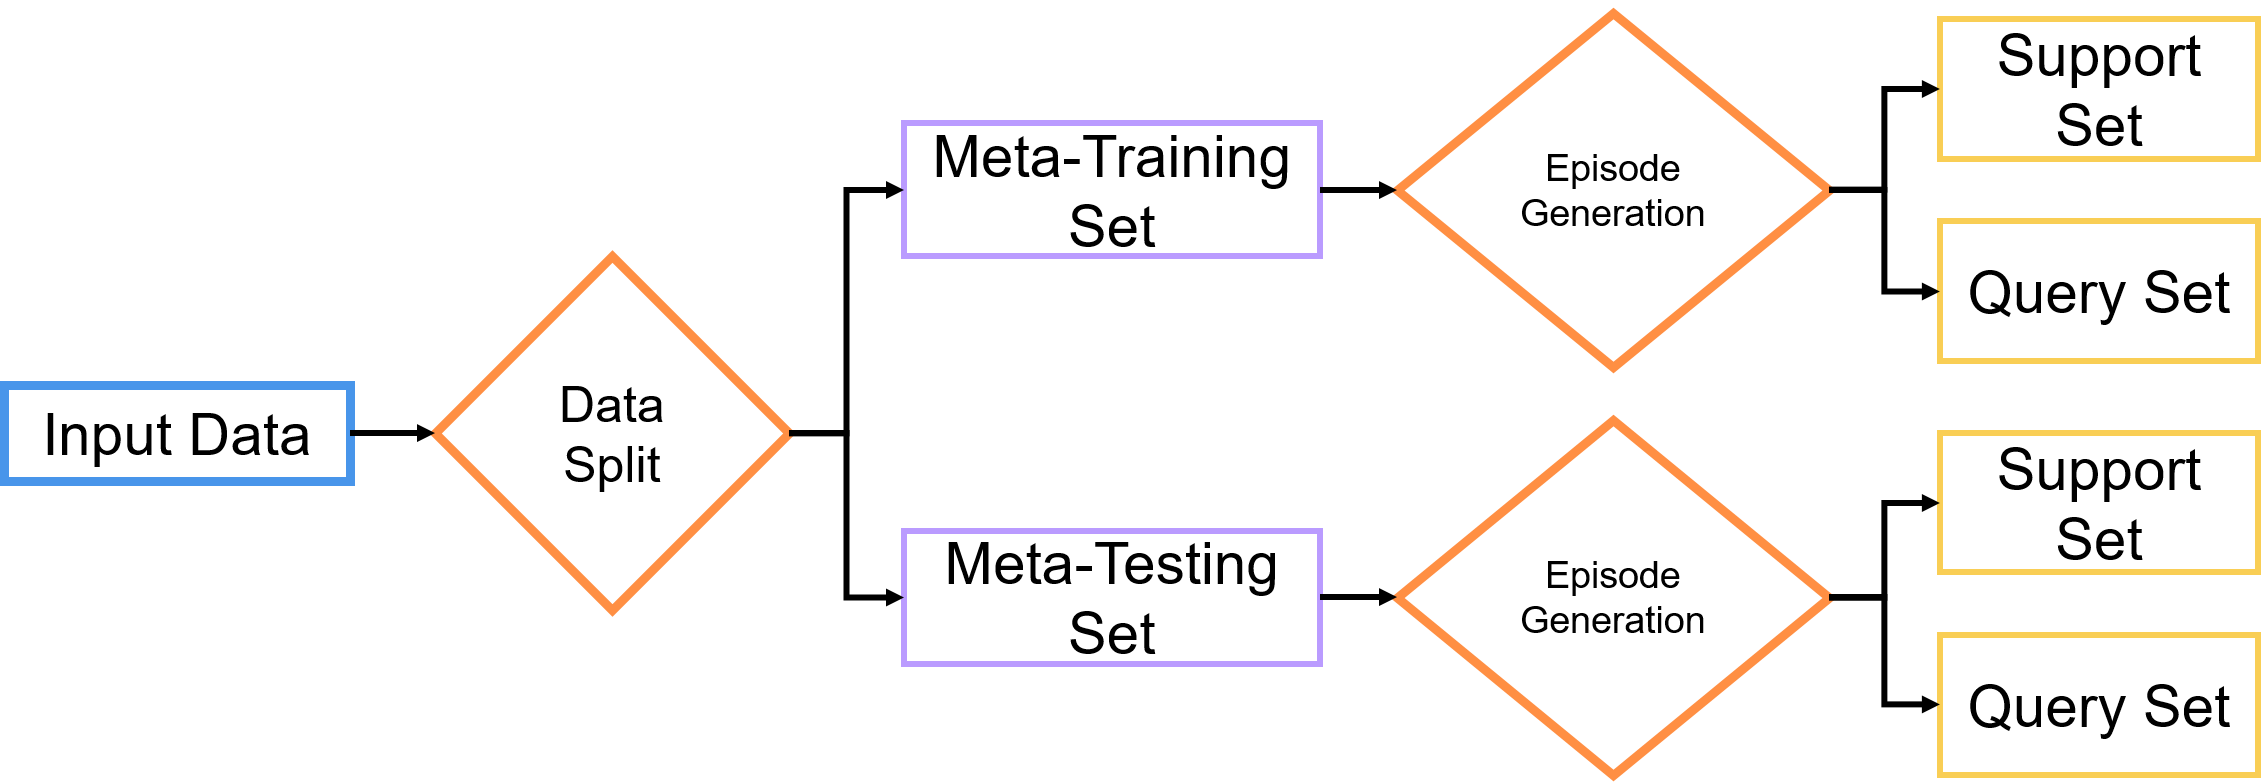
\includegraphics[width=01\linewidth]{Figure_6.png}
    \caption{Few-Shot Learning Workflow Diagram}
    \label{fig:fsl}
\end{figure*}

Transfer learning and fine-tuning approaches have demonstrated effectiveness in FSL applications. \citet{uskaner2024efficient} implemented a strategy using ImageNet pre-trained models fine-tuned on PlantCLEF2022 datasets, achieving 88.4\% accuracy at 10-shots and 75.5\% at 5-shots on PlantVillage data through SVM classification of extracted embeddings. \citet{rezaei2024plant} introduced 5-way 5-shot classification using ViT and ResNet50 with Feature Attention modules, demonstrating ViT superiority with 90.12\% accuracy compared to ResNet50's 76.69\%. \citet{upadhyay2024mango} developed a meta-learning approach for mango crop maturity estimation using DenseNet-121 backbone with Faster R-CNN segmentation, achieving 68.45\% accuracy in 2-way 1-shot and 83.65\% accuracy in 2-way 5-shot scenarios with only 0.7 million trainable parameters, demonstrating superior performance compared to MAML and traditional D-CNN approaches while requiring minimal training data.

Multi-modal and generative approaches have enhanced FSL capabilities. \citet{cao2023cucumber} employed Vision-Language Pre-training for cucumber disease detection, achieving 94.84\% accuracy through image-text contrastive learning integration while maintaining cross-dataset generalization. \citet{argueso2020few} utilized Inception V3 networks combined with Siamese networks and Triplet loss, achieving up to 90.0\% accuracy for 80 shots. \citet{nuthalapati2021multi} implemented transformer-based embeddings with Mahalanobis distance classification, reaching 88.5\% accuracy. \citet{zhong2020zero} employed conditional adversarial autoencoders to transform zero- and few-shot scenarios into supervised tasks, demonstrating competitive performance in challenging conditions.


\subsubsection{Vision Language Models for Enhanced Disease Recognition} \label{sec:vlm}

Vision-Language Models (VLMs) integrate visual perception with textual understanding to create unified frameworks capable of interpreting images and language simultaneously. These architectures enable image description, visual question answering, and zero-shot classification capabilities without task-specific training. VLM architectures typically comprise separate image and text encoders with multimodal fusion mechanisms for cross-modal alignment. Figure \ref{fig:vlm} illustrates the generalized VLM architecture featuring Image Encoders (CNN/ViT), Text Encoders (transformers), and Multimodal Processing units that align and fuse representations through feature alignment and cross-attention mechanisms.

\begin{figure*}[h!]
    \centering
    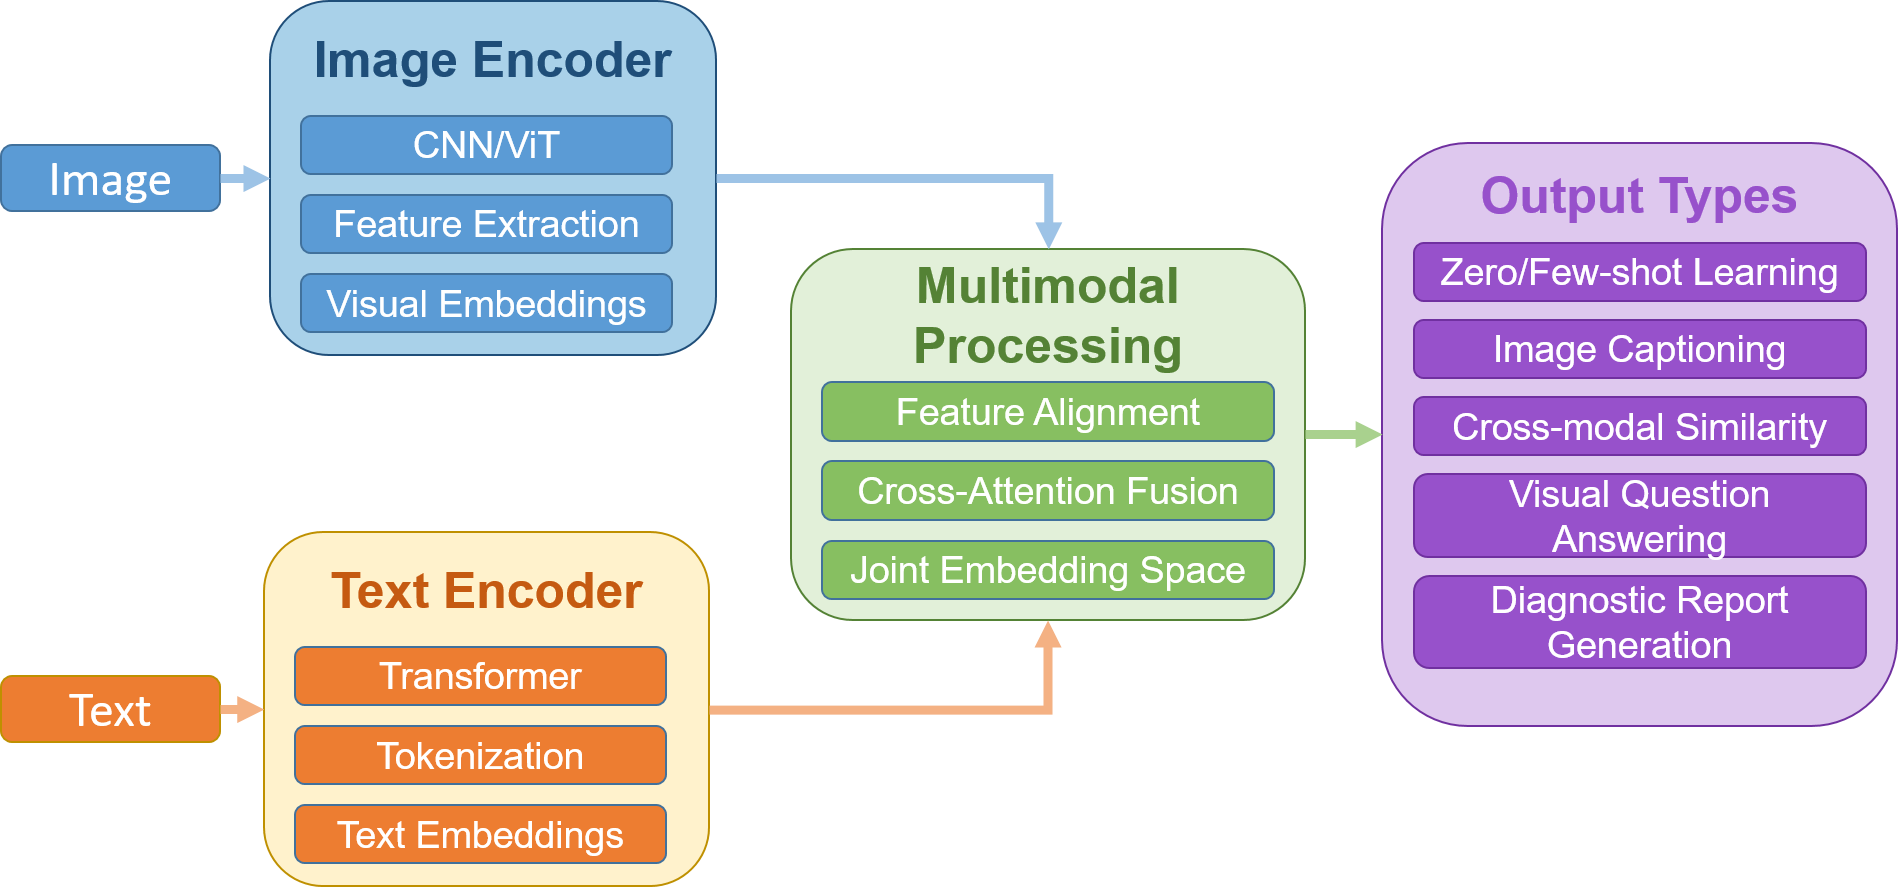
\includegraphics[width=01\linewidth]{Figure_7.png}
    \caption{Generalized Vision-Language Model Architecture for Plant Disease Detection}
    \label{fig:vlm}
\end{figure*}

Agricultural VLM applications have demonstrated particular effectiveness in plant disease identification through visual-textual integration. \citet{zhang2024visual} developed the Wheat Disease Language Model, processing raw images using Grounded-SAM \citep{ren2024grounded} for disease feature segmentation and employing prompt engineering with VLMs to generate detailed descriptions. The model utilizes InternLM-XComposer2 \citep{dong2024internlm} fine-tuning on the specialized Wheat Disease Semantic Dataset (WDSD), enabling mobile deployment for practical field applications. \citet{LI2025106981} proposed ITIMCA (Image-Text Integration with Multi-modal Contrastive Attention), a few-shot learning framework combining CLIP pre-training with cross-attention mechanisms to address agricultural data scarcity, achieving 78.00\% accuracy and 0.79 F1-score for cassava leaf disease recognition under natural conditions through multi-modal contrastive learning integration of visual and textual features.

Anomaly detection approaches have leveraged VLMs for fine-grained disease recognition. \citet{dong2024visual} developed vision-language anomaly detection methods prioritizing visual information over traditional text-based prompts. Their approach achieved 99.85\% AUROC in all-shot settings and 93.81\% in 2-shot scenarios on PlantVillage through maximum concept matching, where test samples from known categories exhibit higher matching scores.

Few-shot classification implementations have addressed limited data scenarios. \citet{zhou2024few} introduced VLCD (Vision-Language Crop Disease) using Qwen-VL \citep{bai2023qwen} to generate textual descriptions of representative disease images selected through clustering. The approach enhanced classifier weight generation with cross-attention mechanisms in training-free modes and Squeeze-and-Excitation attention in training-enabled variants.

Open-vocabulary object detection (OVD) extends VLM capabilities to novel category recognition beyond training distributions \citep{zareian2021open}. \citet{li2024multi} developed PDC-VLD, a multimodal model for tomato leaf disease detection using OVD within the VLDet framework. The model integrates progressive visual transformer-convolutional pyramid modules (PVT-C) for feature extraction and context feature-guided modules (CFG) to enhance performance in data-scarce conditions.

\subsection{Limitation Analysis for Color Imagery-based Plant Disease Detection}
Despite achieving laboratory accuracies of 94-99\% across classical, machine learning, and deep learning methodologies, RGB-based plant disease detection exhibits fundamental constraints that persist across computational generations. While RGB imaging has achieved rapid technological evolution and widespread adoption, systematic limitations continue to restrict reliable agricultural deployment. This analysis examines the persistent constraints that challenge field implementation despite substantial computational advances.

\subsubsection{Environmental Adaptation Constraints}
RGB disease detection methods struggle to maintain laboratory performance under field conditions due to limited spectral information and environmental sensitivity. Illumination dependency makes RGB sensors highly susceptible to lighting variations that affect color perception, with classical methods \citep{arivazhagan2013detection} achieving 94\% accuracy under controlled conditions but demonstrating severe degradation under natural solar variations and shadow patterns. Background interference sensitivity occurs as disease detection relies on color-based discrimination that becomes unreliable with natural backgrounds, soil variations, and seasonal changes, while advanced CNN architectures \citep{ferentinos2018deep} achieving 99.48\% on PlantVillage show poor generalization with complex agricultural backgrounds. Weather-induced degradation through rain, fog, dust, and humidity significantly impacts image quality essential for disease discrimination, with deep learning approaches \citep{atila2021plant} reporting 99.97\% accuracy lacking systematic weather variability evaluation. Laboratory-field performance degradation reaches 22.4\% \citep{yu2023inception} (99.94\% on PlantVillage versus 77.54\% on PlantDoc), demonstrating that environmental standardization systematically excludes natural variability factors including dynamic lighting, weather patterns, and phenological diversity.
\subsubsection{Spectral Information Limitation Constraints}
RGB imaging faces fundamental spectral constraints that limit disease detection capabilities regardless of computational sophistication. Narrow spectral coverage restricts sensors to visible spectrum (400-700 nm), excluding near-infrared and other wavelengths containing critical disease signatures related to cellular structure changes, with machine learning approaches \citep{qin2016identification} extracting 129 features from RGB imagery unable to compensate for fundamental spectral information gaps limiting early detection. Subtle symptom detection failures occur as early disease manifestations involve biochemical changes preceding visible symptoms, requiring spectral sensitivity beyond RGB capabilities, with vision transformer approaches \citep{wu2021multi} achieving 88.1\% accuracy but demonstrating limitations in detecting pre-symptomatic stages where intervention would be most valuable. Disease discrimination ambiguity emerges as multiple diseases produce visually similar symptoms in RGB imagery, creating diagnostic confusion that computational sophistication cannot resolve, while generative approaches \citep{zhang2022mmdgan} achieving high laboratory accuracy face challenges distinguishing between diseases with similar color manifestations but different treatment requirements. Environmental stress confusion occurs as RGB imagery cannot reliably distinguish between biotic disease symptoms and abiotic stress factors (drought, nutrient deficiency, heat stress) that produce similar visual changes, with advanced architectures like CSXAI \citep{prince2024csxai} still suffering from diagnostic ambiguity inherent to limited spectral information.

\subsubsection{Deployment Scalability Limitation}
RGB approaches face escalating trade-offs between computational sophistication and practical deployment requirements, with each methodological generation introducing new scalability challenges. Computational complexity escalation occurs as deep learning architectures require substantial processing power conflicting with agricultural constraints, with vision-language models \citep{zhang2024visual} integrating Grounded-SAM segmentation, prompt engineering, and InternLM-XComposer2 processing, creating overhead incompatible with real-time field processing and resource-constrained environments. Data dependency amplification emerges as advanced methods require extensive labeled datasets that cannot capture agricultural diversity across crops, regions, and conditions, with few-shot learning approaches \citep{uskaner2024efficient} demonstrating critical dependency on support set size (88.4\% at 10-shots versus 75.5\% at 5-shots), indicating limitations when deploying to novel scenarios with limited training data. Model complexity versus interpretability trade-offs manifest as sophisticated architectures achieve accuracy through complex representations lacking agricultural interpretability essential for farmer adoption, with explainable AI techniques \citep{bhandari2023botanicx} requiring technical expertise creating adoption barriers where simplified decision support is essential. Infrastructure dependency barriers arise as advanced RGB systems require high-quality imaging equipment, computational resources, and connectivity unavailable in many agricultural regions, with multi-modal approaches \citep{cao2023cucumber} achieving 94.84\% accuracy through Vision-Language Pre-training creating infrastructure requirements exceeding small-scale farming capabilities where detection systems are most needed.

\subsection{Methodological Evolution in Color Imagery-based Plant Disease Detection}

The chronological analysis of RGB-based plant disease detection methodologies reveals three fundamental paradigm shifts that establish theoretical foundations for next-generation agricultural AI systems. Figure \ref{fig:timelineRGB} demonstrates systematic progression from rule-based image processing to sophisticated neural architectures, illuminating technological forces driving methodological advancement and providing conceptual frameworks for future development trajectories.

\begin{figure*}[h!]
    \centering
    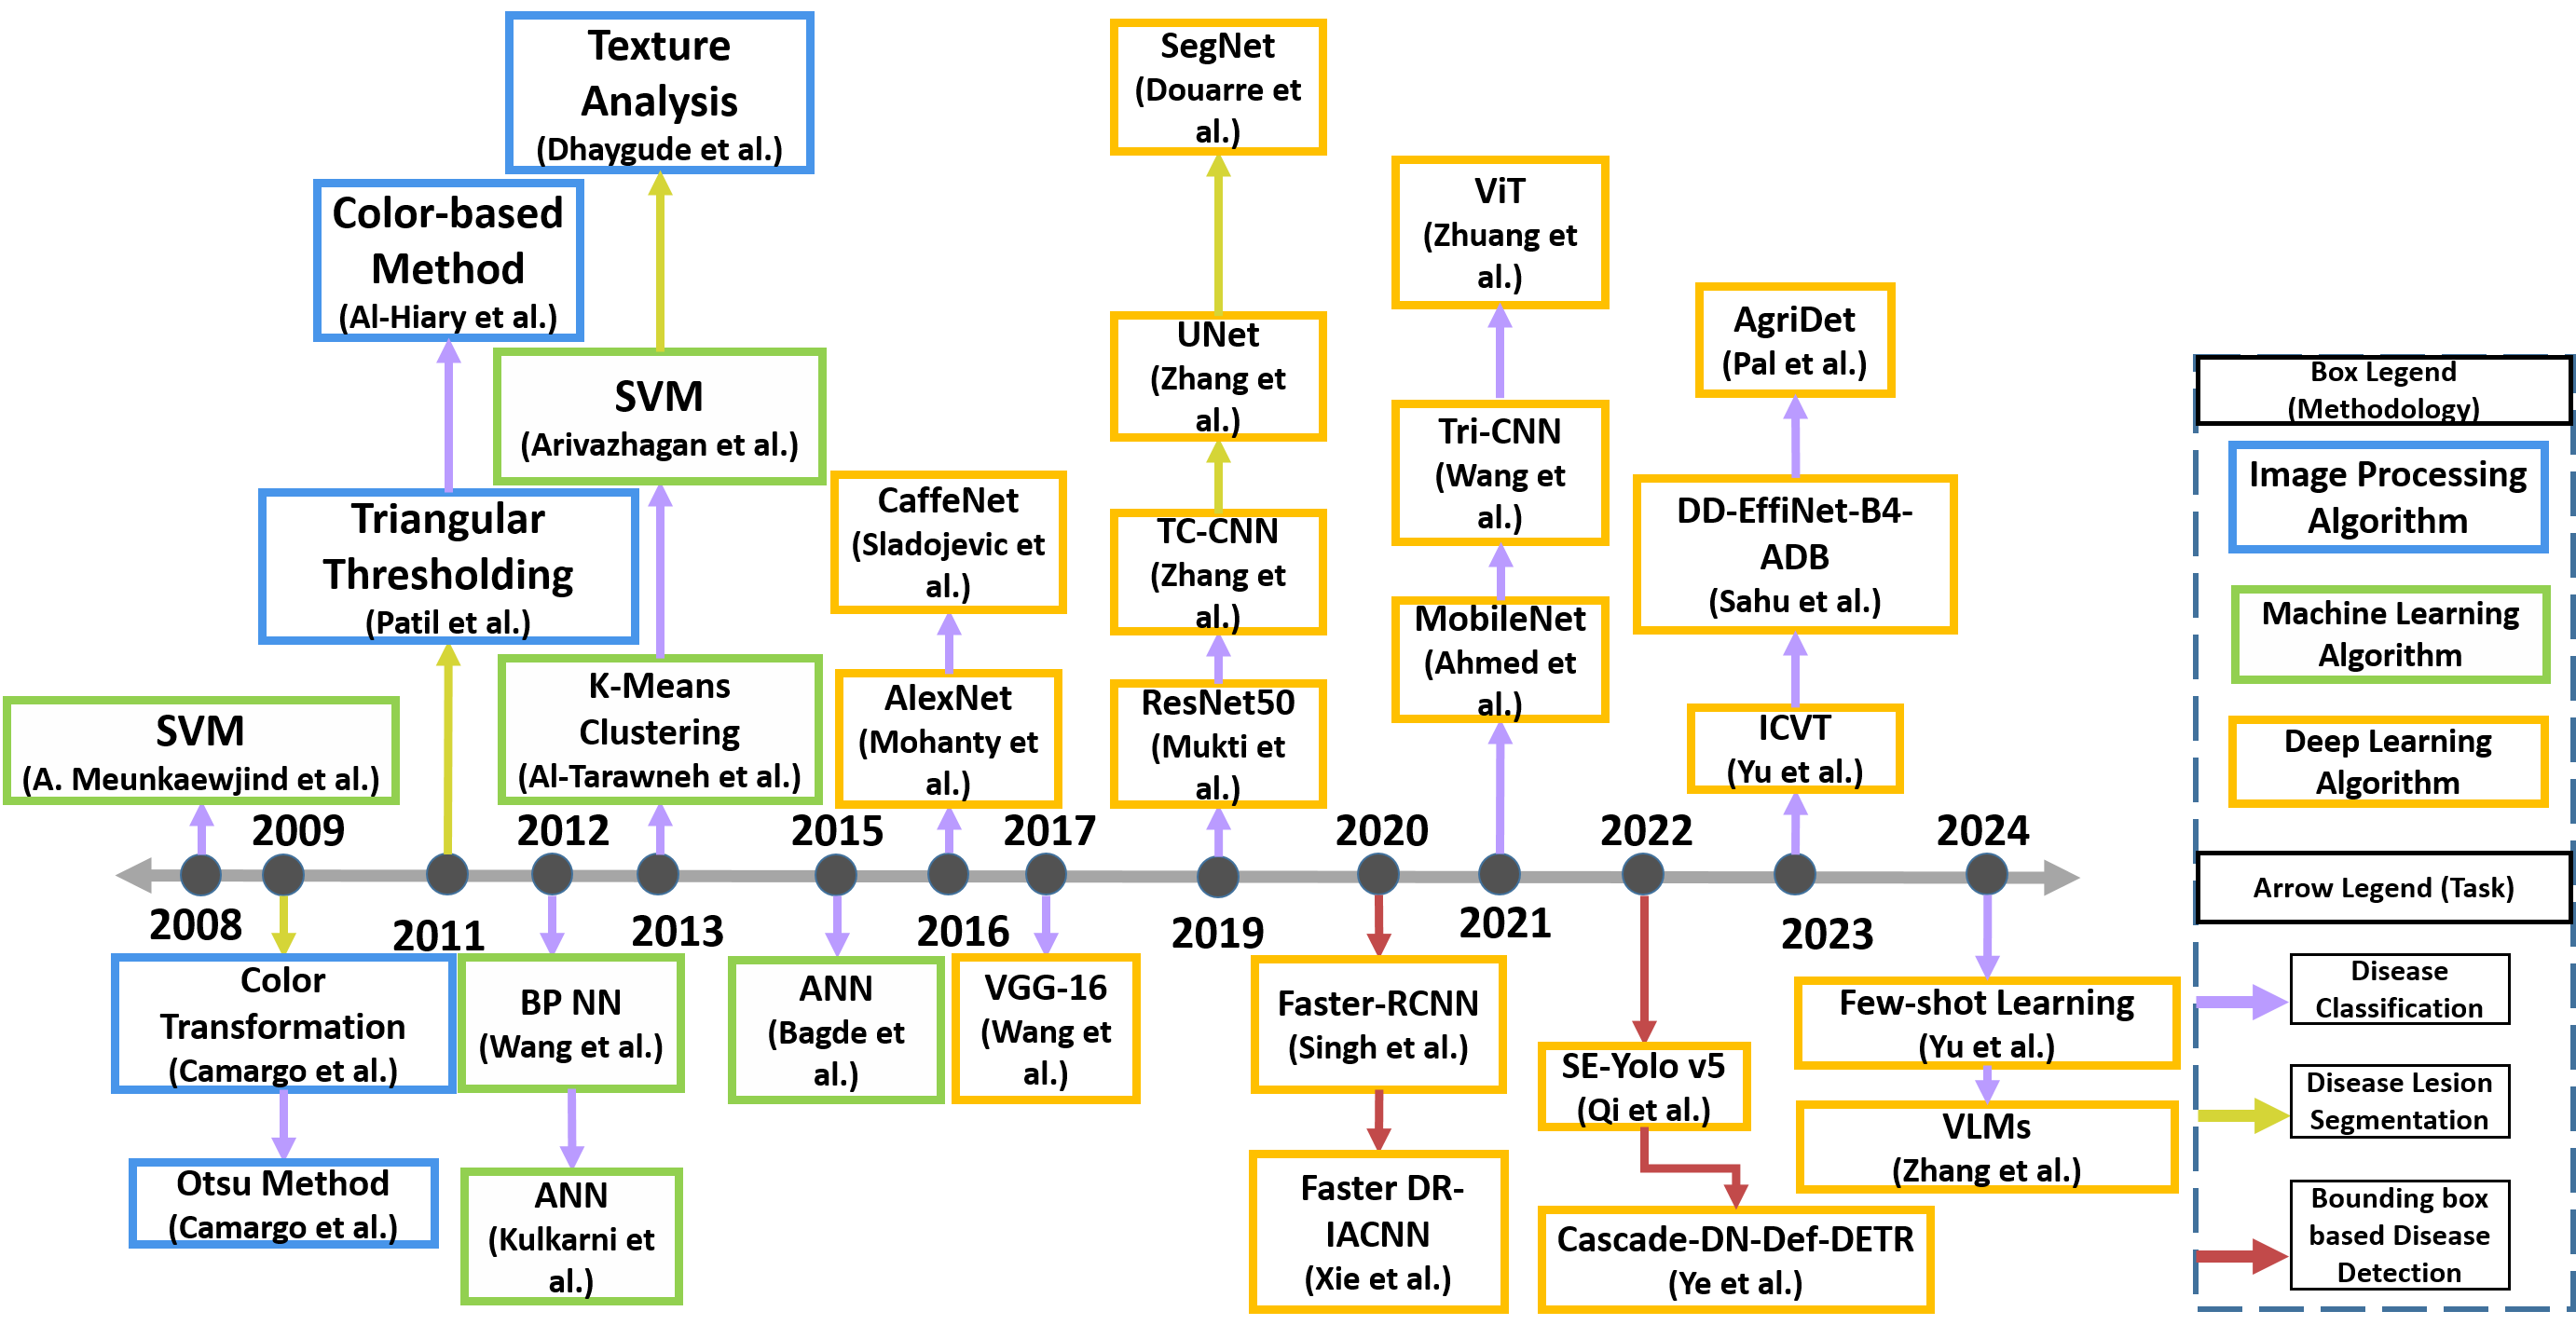
\includegraphics[width=1\textwidth]{Figure_3.png}
    \caption{Chronological overview of the most relevant methodologies for plant disease detection. The color of the box represents the classification of methodology while the color of the arrow shows the task performed. The timeline illustrates the progression of machine learning algorithms in plant disease detection, tracing the developments from foundational methods to advanced techniques involving various neural network architectures, highlighted by the interconnected influences and improvements across different studies}
    \label{fig:timelineRGB}
\end{figure*}

Early methodologies (2008-2015) established agricultural determinism paradigms through classical image processing, treating disease detection as rule-based pattern recognition problems exemplified by color transformation techniques \citep{camargo2009image} and triangular thresholding \citep{patil2011leaf}. The adaptation phase (2015-2020) marked fundamental transition toward statistical agricultural intelligence, where CNN architectures \citep{mohanty2016using, sladojevic2016deep} demonstrated a transition from manual feature engineering to automated agricultural pattern discovery. Contemporary methodologies (2020-2025) exhibit convergence toward multi-modal agricultural cognition, integrating vision transformers \citep{yu2023inception}, few-shot learning \citep{uskaner2024efficient}, and vision-language models \citep{zhang2024visual} that establish frameworks mimicking human cognitive processes through attention mechanisms and cross-modal understanding.


\section{Hyperspectral Approaches to Disease Detection} \label{sec:dlh}
Hyperspectral imaging represents a significant performance-adoption challenge in plant disease detection. While HSI's extended spectral range (250-15,000 nm) enables detection of disease-specific biochemical signatures beyond RGB's limited 380-750 nm range, two decades of research achieving 95-99\% laboratory accuracies have not translated into widespread agricultural deployment. Figure \ref{fig:HSIBand} illustrates this spectral advantage that creates both detection capabilities and deployment challenges. The ability to detect fungal infections through near-infrared tissue structure changes (700-1100 nm), bacterial metabolic alterations in shortwave infrared (1100-2500 nm), and nutrient deficiencies through specific reflectance patterns (nitrogen: 550-650 nm, phosphorus: 430-470 nm) creates information richness that enables precise laboratory detection while complicating practical field implementation \citep{Ali2019}.


\begin{figure*}[h!]
    \centering
    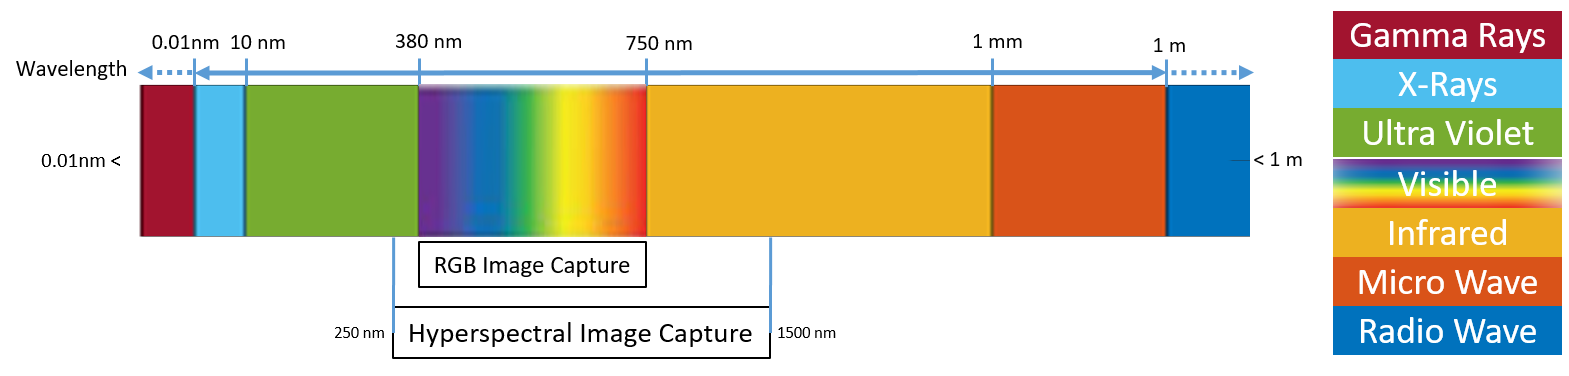
\includegraphics[width=1\linewidth]{Figure_8.png}
    \caption{HSI captures a wide range of wavelengths, spanning from 250 nm to 15,000 nm, while RGB image can capture only visible range from 380 nm to 750 nm}
    \label{fig:HSIBand}
\end{figure*}

Table \ref{tab:hsivsrgb} illustrates deployment characteristics influencing technology adoption in agricultural disease detection. The comparison reveals trade-offs between technical performance and practical implementation requirements. While hyperspectral imaging demonstrates higher accuracy in controlled environments (95-99\% vs. 85-95\% for RGB), several factors limit field deployment: equipment costs are substantially higher (USD10,000+ vs. USD100-1,000), data processing requirements are more intensive (GB vs. MB per sample), and technical expertise demands exceed those of RGB systems \citep{lu2020recent,dichter2020}. RGB systems show wider commercial adoption despite lower spectral resolution, attributed to compatibility with existing infrastructure and reduced operational complexity \citep{gano2024,fu2020}. The performance-deployment gap for HSI systems reflects challenges in translating laboratory advances to field applications, where environmental variability, processing constraints, and cost considerations become determinative factors, informing analysis of technology transfer barriers in precision agriculture.

\begin{table}[h!]
\centering
\small
\caption{Comparative analysis of RGB and hyperspectral imaging deployment characteristics in agricultural disease detection.}
\label{tab:hsivsrgb}
\begin{tabular}{p{3.5cm}p{4cm}p{4cm}}
\hline
\textbf{Deployment Factor} & \textbf{RGB Systems} & \textbf{Hyperspectral Systems} \\
\hline \hline
\textbf{Reported Accuracy} & 85-95\% (field studies) \citep{bendig2014,sanches2018} & 95-99\% (controlled conditions) \citep{lu2020recent,ram2024systematic} \\ 
\hline
\textbf{Current Adoption} & Commercial deployment \citep{gano2024,fu2020} & Primarily research-based \citep{lu2020recent,ram2024systematic} \\ 
\hline
\textbf{Equipment Cost} & USD100-1,000 \citep{dichter2020,spanos2023} & USD10,000+ \citep{lu2020recent,imec2024,dichter2020} \\ 
\hline
\textbf{Operator Requirements} & Basic training \citep{livingoptics2024} & Spectral analysis expertise \citep{lu2020recent} \\ 
\hline
\textbf{Processing Speed} & Real-time capable \citep{gano2024} & Computationally intensive \citep{lu2020recent,imec2024} \\ 
\hline
\textbf{Environmental Robustness} & Field-validated performance \citep{gene2020assessing} & Variable field performance \citep{lu2020recent,ram2024systematic} \\ 
\hline
\textbf{Data Requirements} & 3MB per image \citep{gano2024} & GB datacubes \citep{lu2020recent,ram2024systematic} \\ 
\hline
\textbf{Detection Capability} & Visible symptom identification \citep{livingoptics2024} & Pre-symptomatic detection potential \citep{lu2020recent} \\ 
\hline
\textbf{User Interface} & Visual interpretation \citep{gano2024} & Requires spectral analysis \citep{ram2024systematic,lu2020recent} \\ 
\hline
\textbf{Integration Requirements} & Standard agricultural hardware \citep{fu2020} & Specialized sensor systems \citep{imec2024,lu2020recent} \\
\hline
\end{tabular}
\end{table}
Figure \ref{fig:HSI_pipeline} depicts the hyperspectral imaging processing workflow for plant disease detection, highlighting the computational and operational requirements at each stage. The pipeline encompasses spectral data acquisition, preprocessing (including atmospheric correction and reflectance calibration), dimensionality reduction through principal component analysis, and classification algorithms. Each processing step introduces specific technical requirements: specialized sensor calibration, expertise in spectral preprocessing, computational resources for high-dimensional data analysis, and algorithm optimization for agricultural conditions \citep{lu2020recent}. The performance of the workflow depends on controlled acquisition conditions, including stable illumination and precise sensor calibration, which may vary in field environments compared to laboratory settings. The disparity between laboratory and field performance can be attributed to environmental variability, processing constraints, and the complexity of translating multi-stage pipelines to real-time agricultural applications. Understanding these pipeline requirements provides context for evaluating the practical implementation of HSI systems in precision agriculture.

\begin{figure*}[h!]
    \centering
    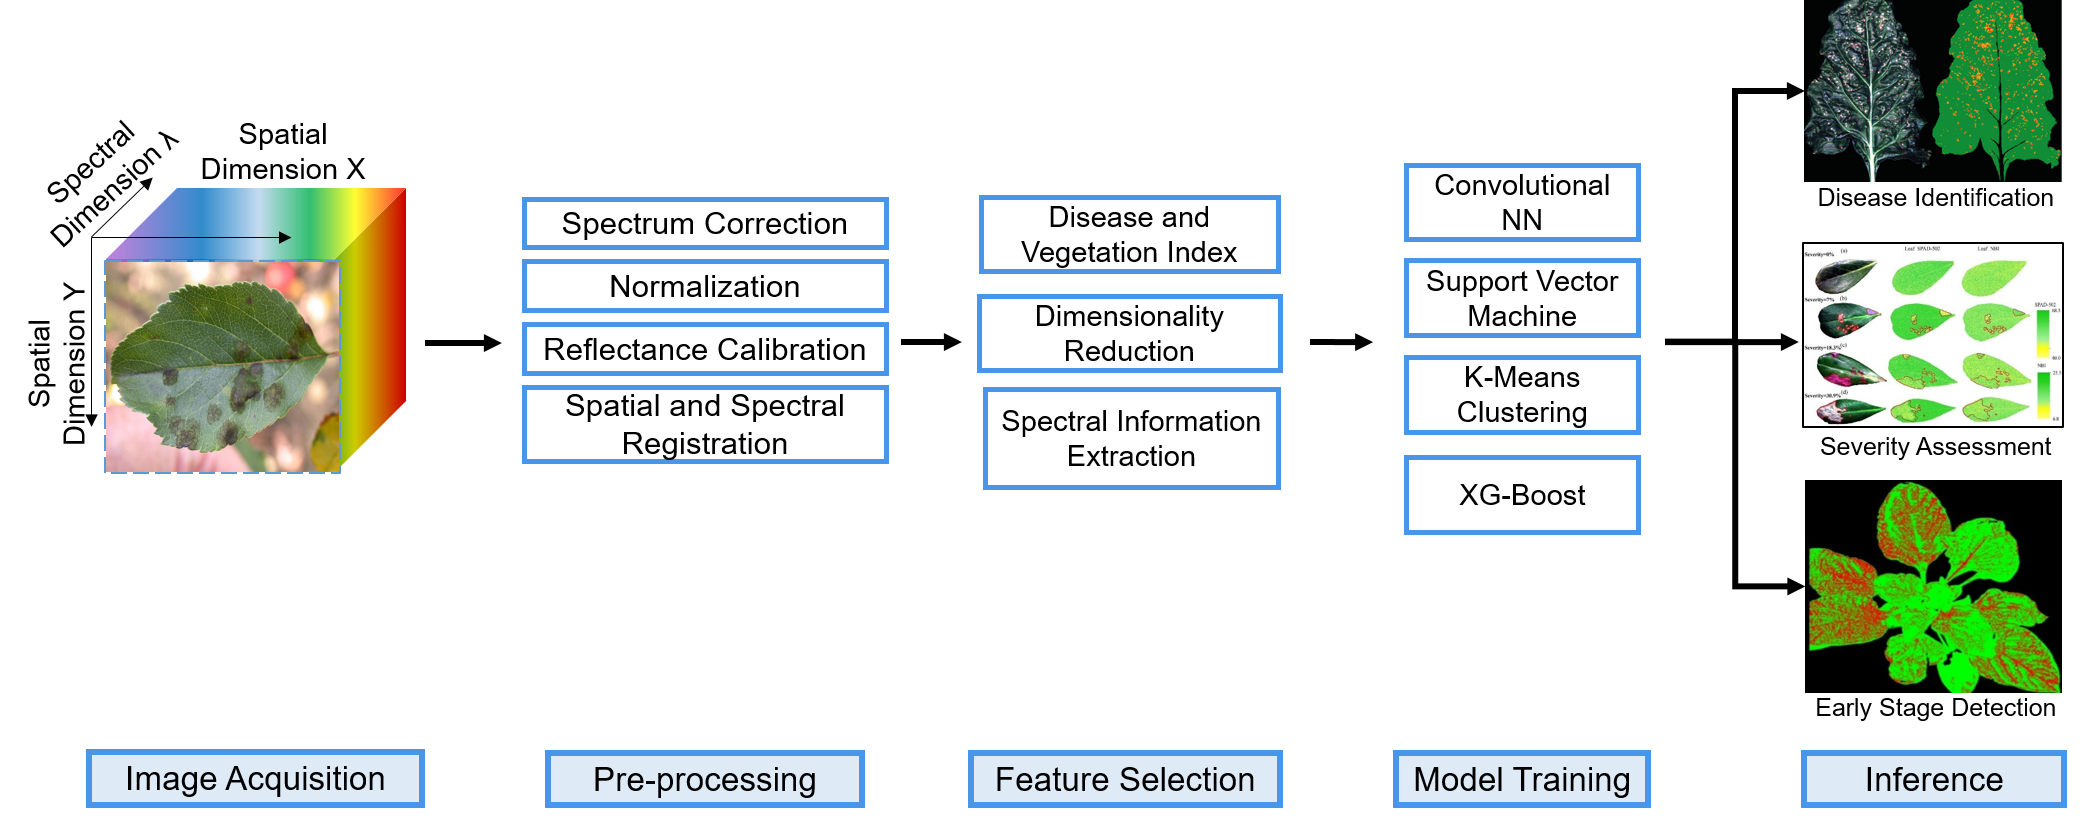
\includegraphics[width=1\textwidth]{Figure_9.png}  
    \caption{Visual representation of a plant disease detection process using spectral analysis and machine learning. The leftmost image cube symbolizes the extraction of spectral features from diseased leaf imagery, which are then fed into a layered CNN architecture for feature learning and classification, with the output being disease identification \citep{mahlein2016plant}, severity assessment \citep{jiang2021assessing}  or early stage detection \citep{moghadam2017plant}}
    \label{fig:HSI_pipeline}
\end{figure*}

The following sections examine the evolution of hyperspectral imaging methodologies from classical spectral analysis through machine learning to deep learning approaches. This analysis evaluates how methodological advances have addressed deployment challenges and identifies persistent barriers to widespread field implementation. Rather than solely reviewing technical developments, the discussion assesses the relationship between algorithmic sophistication and practical applicability in agricultural settings. The examination considers whether increased computational complexity has corresponded with improved field deployment outcomes, and explores factors that influence the translation of laboratory advances to operational agricultural systems.

\subsection{Traditional Hyperspectral Processing}
Classical computer vision techniques established the foundational promise of HSI disease detection while simultaneously revealing systematic limitations that constrain all subsequent methodological generations. This section examines how classical approaches achieved remarkable laboratory accuracies (99-100\%) through direct spectral analysis, dimensionality reduction, and index-based simplification, while their systematic deployment failures revealed core constraints that persist across two decades of computational advancement.

\subsubsection{Direct Spectral Signature Analysis}
Spectral signature analysis established the theoretical foundation for HSI disease detection through comprehensive laboratory investigations. \citet{huang2020measurement} developed early fungal disease detection protocols for blueberries, utilizing 400 samples with partial least squares discriminant analysis (PLSDA) applied to hyperspectral data. Their methodology emphasized wavelengths beyond 685 nm, particularly in the near-infrared spectrum, achieving 99\% classification accuracy for healthy samples and 100\% for early diseased specimens. \citet{lu2018using} implemented a comprehensive approach for tomato yellow leaf curl virus detection, employing reflectance spectroscopy combined with band ratio analysis. Their protocol integrated texture analysis methods including ROC curve evaluation and Gray Level Co-occurrence Matrix (GLCM) analysis, achieving an optimal AUC value of 1.0 using the 720/840 nm band ratio. \citet{li2022classification} developed diagnostic protocols for Pine Wilt Disease detection in Japanese and Korean pine trees through systematic identification of key diagnostic spectral bands, applying Linear Discriminant Analysis (LDA) for classification and achieving 77\% and 78\% accuracy for healthy and infected trees, respectively.


\subsubsection{Spectral Feature Selection}

Classical feature selection approaches sought to leverage HSI's spectral richness while addressing computational complexity through systematic dimensionality reduction. \citet{whetton2018hyperspectralP1} developed comprehensive detection protocols for Fusarium head blight and yellow rust in wheat and barley, implementing Principal Component Analysis (PCA) and Partial Least Squares Regression (PLSR) for spectral data processing. Their controlled laboratory methodology achieved R² values ranging from 0.75 to 0.95 for Fusarium head blight detection and 0.76 to 0.92 for yellow rust identification, though performance varied significantly across different growth stages. Field validation studies \citep{whetton2018hyperspectralP2} revealed substantial performance variations, with yellow rust detection declining to R² values between 0.72 and 0.78, while Fusarium head blight detection dropped to R² values between 0.61 and 0.82, representing up to 36\% performance degradation from optimal laboratory conditions. 


\citet{skoneczny2020fire} implemented hyperspectral remote sensing protocols for Fire Blight identification in apple trees, utilizing Analysis of Variance (ANOVA) and spectral indices to systematically evaluate discriminative capabilities across the electromagnetic spectrum. Their methodology identified NIR-SWIR bands from 850 to 2500 nm as most discriminative, with specific bands at 1450 and 1900 nm demonstrating strong disease-indicative responses. \citet{jones2010diagnosis} developed spectroscopic assessment protocols for tomato leaf spot severity quantification, implementing Stepwise Multiple Linear Regression (SMLR) and Partial Least Squares (PLS) regression analysis. Their approach achieved R² = 0.82 with RMSD = 4.9\% in validation datasets, identifying chlorophyll absorption wavelengths as most diagnostic for disease severity assessment.


\subsubsection{Index-Based Simplification Approaches}

Spectral vegetation indices represent systematic attempts to distill complex hyperspectral signatures into interpretable scalar metrics for disease detection applications. \citet{abdulridha2020laboratory} developed index-based classification protocols for tomato diseases, implementing Modified Triangular Vegetation Index 1 (MTVI1) and Renormalized Difference Vegetation Index (RDVI) for disease discrimination. Their controlled laboratory methodology achieved 100\% classification accuracy across multiple tomato disease categories. \citet{abdulridha2020detection} expanded index-based approaches through comprehensive evaluation of multiple spectral indices including Photochemical Reflectance Index (PRI), Normalized Difference Vegetation Index (NDVI), Triangular Vegetation Index (TVI), and Chlorophyll Green Index. Their laboratory protocols achieved classification accuracies between 97\% and 99\% for distinguishing between morphologically similar tomato diseases.


\subsection{Machine Learning Integration with Hyperspectral Data}

Machine learning integration with hyperspectral imaging represents a systematic attempt to overcome the limitations presented by classical methods through automated pattern recognition and sophisticated feature extraction capabilities. These approaches encompass classification-based disease detection, regression-based severity assessment, and feature reduction methodologies that demonstrate substantial laboratory performance improvements over traditional spectral analysis techniques. However, systematic evaluation reveals that machine learning methods, despite computational sophistication, exhibit deployment constraints that mirror the fundamental limitations established by classical approaches. This section examines whether data-driven methodologies successfully address the environmental robustness, information-complexity balance, and temporal generalization requirements critical for agricultural deployment, or whether they amplify existing constraints through increased computational complexity and data dependency.

\subsubsection{Classification-Based Disease Detection}
\textbf{Research Contributions and Methodological Approaches}
Machine learning classification methods represent systematic attempts to automate pattern recognition in hyperspectral disease detection through supervised learning algorithms. \citet{abdulridha2019uav} implemented UAV-based spectral vegetation index analysis for citrus canker detection in tangerines, integrating aerial data acquisition with automated classification protocols. \citet{cheshkova2023application} applied Support Vector Machine (SVM) and K-Nearest Neighbors (KNN) algorithms for fungal infection discrimination on strawberry leaves, with SVM demonstrating superior classification performance. \citet{alisaac2018hyperspectral} employed SVM classification for Fusarium head blight detection in wheat, achieving 99\% accuracy while identifying significant spectral vegetation indicators for disease discrimination. \citet{rumpf2010early} implemented SVM-based classification protocols for sugar beet leaf health assessment, achieving 86\% accuracy in healthy versus infected leaf discrimination. \citet{calamita2021early} evaluated multiple machine learning algorithms for early grapevine disease detection, with Naïve Bayes classification demonstrating optimal performance. \citet{sankaran2013huanglongbing} utilized SVM classification for Huanglongbing detection in citrus trees, achieving 87\% discrimination accuracy. \citet{lan2020comparison} implemented AdaBoost ensemble classification methods for HLB identification in citrus trees using multispectral UAV data, achieving 100\% classification accuracy.


\subsubsection{Regression-Based Severity Assessment}
Regression methodologies enable quantitative disease severity assessment by establishing mathematical relationships between hyperspectral reflectance patterns and continuous disease severity scales, typically ranging from 0\% (healthy) to 100\% (fully diseased). The machine learning process involves training algorithms on hyperspectral data paired with expert-assessed severity ratings, enabling automated prediction of disease progression stages from spectral signatures. R² correlation coefficients measure the proportion of severity variance explained by spectral predictors, where values approaching 1.0 indicate strong predictive relationships between reflectance patterns and disease intensity levels.

\citet{lu2019evaluating} established theoretical frameworks for applying regression models to disease progression analysis and chlorophyll content estimation from hyperspectral signatures. \citet{feng2022hyperspectral} developed comprehensive monitoring protocols for wheat powdery mildew severity assessment, implementing Random Forest (RF) Regression with systematic preprocessing and feature extraction techniques. Their methodology focused on specific spectral bands during flowering stages, achieving R² values of 0.849–0.852 for severity estimation, indicating that spectral features explained 84.9-85.2\% of disease severity variance. \citet{jiang2023monitoring} implemented hyperspectral differentiation and severity assessment protocols for apple leaf mosaic disease, identifying significant spectral responses at 702 nm wavelength. Their comparative evaluation of RF and Variable Projection eXtreme Gradient Boosting (VPs-XGBoost) models demonstrated superior performance with VPs-XGBoost achieving R² = 0.849 for anthocyanin content estimation and disease severity monitoring.


\subsubsection{Feature Reduction and Wavelength Selection}
Feature reduction methodologies address the computational challenges inherent in high-dimensional hyperspectral data by identifying optimal spectral subsets while preserving disease-diagnostic information. Machine learning algorithms facilitate this process through automated feature selection and dimensionality reduction techniques that transform hundreds of spectral bands into manageable feature sets for disease detection applications.
\citet{zhao2020identification} implemented Principal Component Analysis (PCA) for hyperspectral dimensionality reduction, enabling computational efficiency improvements and enhanced classification accuracy. \citet{liu2021classification} developed integrated feature selection protocols for Frogeye Leaf Spot detection in soybeans, combining Competitive Adaptive Reweighted Sampling (CARS) with PCA for wavelength selection and data reduction, achieving 97.3\% accuracy with SVM and LS-SVM models. \citet{lu2018detection} applied PCA with 57 spectral vegetation indices -for tomato disease detection, achieving near 100\% accuracy for late-stage and healthy leaves while experiencing accuracy degradation to 65.2\% for asymptomatic leaves. \citet{xie2015detection} employed Successive Projections Algorithm for key wavelength identification in tomato early and late blight detection, achieving 97.1-100\% accuracy with Extreme Learning Machine (ELM) classification. \citet{MOSHOU200575} implemented real-time feature reduction for yellow rust detection in winter wheat, combining hyperspectral data with fluorescence imaging and achieving 94.5\% discrimination accuracy through Quadratic Discriminant Analysis. \citet{shuaibu2018unsupervised} utilized Orthogonal Subspace Projection (OSP) for Apple Marssonina blotch detection, reducing 437 spectral bands (356-1000 nm) to ten optimal bands primarily in the 921-957 nm range, achieving 84.3\% classification accuracy with ensemble bagged classifiers across five disease severity classes.
Machine learning integration with HSI demonstrates systematic constraints that mirror classical method limitations despite computational sophistication. Classification approaches achieve high laboratory accuracy (86-100\%) through algorithm-specific overfitting rather than robust pattern learning. Regression methods exhibit temporal specificity limitations and correlation-causation interpretation errors that compromise field applicability. Feature reduction techniques create information loss-efficiency limitations that eliminate spectral diversity essential for environmental robustness. These constraints reveal that machine learning approaches amplify rather than resolve the fundamental deployment challenges established by classical methods, indicating that computational advancement alone cannot overcome the core trade-offs between laboratory performance and agricultural robustness requirements.

%%%%%%%%%%%%%%%%%%%%%%%DL%%%%%%%%%%%%%%%%%%%%%%%


\subsection{Deep Learning Architectures for Hyperspectral Disease Analysis}
Deep learning methodologies represent the most computationally sophisticated approaches to hyperspectral disease detection, employing multi-layered neural architectures for automated feature extraction and pattern recognition from high-dimensional spectral data. These approaches promise to overcome machine learning limitations through hierarchical feature learning, nonlinear mapping capabilities, and end-to-end optimization that eliminates manual feature engineering requirements. 

\subsubsection{Convolutional Neural Networks for Disease Classification}
Deep learning classification methods represent advanced pattern recognition approaches employing multi-layered neural architectures for automated feature extraction from high-dimensional hyperspectral data. \citet{jia2023net} developed Y-Net, a 3D-2D hybrid CNN architecture integrating spatial and spectral feature processing for corn leaf disease detection, achieving 98.34\% classification accuracy through combined convolutional operations. \citet{liu2020disease} implemented 1D-CNN frameworks for potato disease classification using hyperspectral data, achieving 97.22\% accuracy with improved processing speed compared to conventional SVM approaches. \citet{gao2023detection} developed multidimensional fusion Atrous-CNN architectures for potato disease detection, achieving 99.83\% accuracy through five-fold cross-validation by incorporating dilated convolutions for multi-scale feature extraction. \citet{nagasubramanian2019plant} utilized CNN architectures for charcoal rot diagnosis in soybean crops, achieving 95.73\% accuracy through deep feature learning from hyperspectral signatures. \citet{jin2018classifying} implemented pixel-wise classification protocols for wheat head disease detection using hyperspectral images (1620×2325 pixels, 400-1000 nm, 339 wavebands) with preprocessing through mean removal and background-healthy-diseased classification schemes.

Recent developments demonstrate continued architectural refinement while revealing persistent deployment constraints. \citet{xie2024hyperspectral} implemented multi-camera hyperspectral detection systems for wheat crown rot using VNIR, SWIR, and full-spectrum configurations. SVM model achieved F1 scores of 0.75-0.86 at 30-40 days post-infection through optimal data transformation protocols including standard normal variate and hyper-hue preprocessing. Their wavelength optimization identified 26 critical bands (450-2400 nm) enabling lightweight multispectral camera development, demonstrating that VNIR systems detect early photosynthetic changes while SWIR cameras provide superior sensitivity to water and nutrient distribution alterations during advanced infection stages. \citet{yu2025detection} proposed dual-branch CNN architectures combining spatial and spectral processing for citrus fungal disease detection, implementing CARS algorithm for dimensionality reduction from 224 to 44 critical spectral bands while achieving 92.50\% accuracy for distinguishing quarantine disease Phytophthora syringae from similar non-quarantine diseases. \citet{liu2025early} developed Multi-Scale Integrator Selection Attention Transformer Network (MS-STNet) combining UAV hyperspectral imagery with Rice Blast Texture Indices, achieving 96.98\% accuracy through multi-year validation across natural and artificial infection scenarios using multi-scale feature extraction with top-k attention mechanisms. \citet{swaraj2025xception} proposed Xception-Deep Kronecker Network (Xception-DKN) integrating multiple optimization algorithms (FWWPDO, BHEFC) for grape leaf disease severity classification, achieving 92.204\% accuracy.


\subsubsection{Deep Learning Techniques for Disease Severity Assessment}
Deep learning severity assessment methodologies enable continuous disease progression quantification through advanced neural architectures designed for multi-class severity classification and stage identification. \citet{li2023intelligent} implemented enhanced Mask R-CNN techniques combined with prototype networks for Pine Wilt Disease (PWD) infection stage categorization in individual trees using remote sensing data, achieving 83.51\% overall accuracy for identifying and classifying multiple infection progression levels. \citet{yadav2022citrus} developed VGG-based CNN architectures for citrus fruit disease severity classification across different diseases and peel conditions using hyperspectral imaging, implementing Principal Component Analysis (PCA) for crucial band selection and achieving exceptional performance metrics (accuracy: 99.84\%, sensitivity: 99.84\%, specificity: 99.98\%). \citet{rana2024comprehensive} conducted a comprehensive evaluation of SIFT and RANSAC-based multispectral image registration strategies in heterogeneous agricultural environments containing Triticum aestivum and Raphanus raphanistrum, demonstrating that binary mask-based registration achieved the highest accuracy (mean IoU 0.8314) compared to masked pixel registration (0.8183) and spatial realignment of annotations (0.8055), with YOLOv8l-seg achieving 92.11\% mAP@0.5 for wild radish detection.
Recent developments demonstrate enhanced biochemical integration approaches while revealing persistent severity assessment limitations. \citet{ban2025evaluation} integrated hyperspectral imaging with biochemical parameter analysis to establish quantitative relationships between secondary metabolites (flavonoids: r=-0.523, anthocyanins: r=-0.746) and spectral signatures for lettuce downy mildew detection, achieving ultra-early detection within 24 hours post-infection using PLS, RF, and CNN models for predicting disease index, flavonoids, and anthocyanins with high accuracy (R² up to 0.963). This approach establishes a biochemical resistance paradigm for non-destructive resistance screening and germplasm evaluation, though cross-seasonal stability of biochemical-spectral relationships remains unvalidated.

\subsubsection{Transfer Learning and Early Detection Methods}

Early disease detection methodologies leverage deep learning architectures for pre-symptomatic pathogen identification, enabling intervention before visible symptom manifestation. \citet{nguyen2021early} implemented pixel-wise classification protocols for grapevine viral infection detection during asymptomatic stages using hyperspectral imaging, achieving 95\% classification accuracy through SVM, RF, and PCA ensemble approaches. \citet{yu2021three} employed 3D CNN architectures for early Pine Wilt Disease (PWD) detection in forest trees, achieving 88.11\% overall accuracy while demonstrating reduced performance (51.97\%) specifically for early diseased tree identification. \citet{feng2021hyperspectral} implemented deep transfer learning methodologies for rice disease diagnosis across multiple disease types, achieving over 88\% accuracy through fine-tuning approaches that adapt pre-trained models to specific agricultural pathology applications.

Recent developments demonstrate advanced early detection approaches while revealing persistent pre-symptomatic challenges. \citet{zhang2024hyperspectral} established quantitative relationships between hyperspectral signatures and bacterial pathogen populations ($10^5$ to $10^8$ CFU/cm²) for pre-symptomatic tomato bacterial leaf spot detection using LDA, identifying critical wavelengths corresponding to water-soaking effects (1400 nm) and defense hormone responses (750 nm) during early infection stages. Their methodology demonstrated that vegetation index categorization into physiological groupings (pigment, stress response, structure, water content) improved classification performance by 26-37\% over raw spectral data while providing biological interpretability for disease progression mechanisms. \citet{song2025early} integrated solar-induced chlorophyll fluorescence (SIF) with hyperspectral reflectance using three-band Fraunhofer line discrimination method, achieving superior early detection sensitivity (SIF-A correlation: -0.781) compared to traditional vegetation indices for wheat powdery mildew monitoring, demonstrating that SIF+VI fusion in RBF models enables early diagnosis during disease lag phase across different wheat varieties and nitrogen fertilizer levels. \citet{tan2025early} developed novel recurrence plot transformation approaches converting 1D hyperspectral curves into 2D spatial patterns for pre-symptomatic Verticillium wilt detection in cotton, achieving 96.3\% accuracy in distinguishing healthy, asymptomatic, and symptomatic states by extracting texture features from spectral recurrence plots using Gray-Level Gradient Co-occurrence Matrix, enabling early intervention during cryptic infection phases.

\subsubsection{Unsupervised Learning and Feature Extraction}

Unsupervised learning methodologies address labeled data scarcity through automated pattern discovery and feature extraction from hyperspectral signatures without requiring extensive manual annotation. \citet{zhang2022banana} implemented comparative evaluation of unsupervised techniques (ISODATA, Hotspot Analysis) versus supervised methods (SVM, RF, Backpropagation NN, LR) for Banana Fusarium Wilt identification using UAV-captured multispectral images, achieving optimal performance (97.28\%) with RF using five-band imagery while demonstrating that Hotspot Analysis achieved 95\% accuracy for late-stage detection using vegetation indices (WDRVI, NDVI, TDVI). \citet{zhou2017non} employed Deep Belief Networks (DBN) combined with backpropagation classifiers for moldy core severity classification in apples across five disease stages, achieving 88\% accuracy using 150 training and 75 testing samples. \citet{sun2018classification} implemented DBN with PCA integration for peach disease categorization using spectral and spatial characteristics, achieving progressive accuracy improvements across severity stages (initial: 82.5\%, moderate: 92.5\%, severe: 100\%).

Recent developments demonstrate advanced spectral unmixing approaches while revealing persistent unsupervised learning approaches. \citet{jeong2025spectral} developed spectral unmixing methodologies using Purity Pixel Index algorithms to extract 8 universal endmembers from 378 hyperspectral images across six pine species, achieving differentiation between pine wilt nematode infection and natural seasonal color changes with sub-pixel endmember analysis providing earlier detection (4 weeks ahead of NDVI) and enabling cross-species transferability for distinguishing biotic stress from natural phenological processes.

\subsection{Limitation Analysis for HSI-based Plant Disease Detection}

Despite achieving consistent laboratory accuracies of 95-99\% across two decades of methodological evolution, hyperspectral imaging for plant disease detection exhibits three fundamental constraints that persist across all computational generations. Analysis of current methodologies reveals persistent limitations that restrict practical deployment despite advances in computational techniques. This section examines the fundamental constraints that continue to challenge field implementation of hyperspectral disease detection systems.

\subsubsection{Environmental Robustness Constraints}
Hyperspectral disease detection methods demonstrate performance degradation under operational field conditions due to environmental variability excluded during laboratory optimization. These constraints manifest across methodological generations through several mechanisms. Atmospheric interference affects diagnostically valuable spectral regions, particularly the 720/840 nm ratio and extended NIR range, which exhibit susceptibility to water vapor, solar angle effects, and aerosol scattering, while \citet{song2025early} showed that advanced methods like SIF+VI fusion require specialized equipment exceeding typical agricultural deployment capacity. Illumination geometry dependencies cause MTVI1 and PRI indices to show high sensitivity to lighting variations eliminated in laboratory conditions but unavoidable in field applications, with CNN architectures trained on laboratory-specific illumination patterns demonstrating poor generalization under variable field lighting. Canopy structure interference creates systematic calibration errors through atmospheric scattering and architecture variations that cause temporal index variations exceeding disease-related spectral changes, persisting through modern approaches where \citet{tan2025early} demonstrated that recurrence plot transformations require computational overhead conflicting with real-time processing requirements. \citet{whetton2018hyperspectralP2} reported laboratory-to-field performance degradation reaching 36\%, with advanced CNN architectures showing similar degradation patterns during controlled-to-operational transitions due to environmental standardization protocols that systematically exclude atmospheric, illumination, and phenological variability inherent to agricultural environments.


\subsubsection{Temporal Generalization Limitations}
Hyperspectral methods exhibit systematic performance degradation across temporal scales, indicating fundamental temporal instability that computational sophistication cannot overcome. Phenological specificity failures occur because analytical frameworks treat disease-specific spectral signatures as temporally invariant, neglecting dynamic plant-pathogen interactions across growth stages. Machine learning methods demonstrate this limitation, with \citet{feng2022hyperspectral} achieving high performance in flowering-stage optimization (R² = 0.849-0.852) under specific phenological conditions but requiring revalidation across different growth periods. Seasonal relationship instability emerges despite \citet{ban2025evaluation} establishing high correlations between secondary metabolites and spectral signatures (R² up to 0.963), as these relationships require validation across seasonal variations to ensure temporal stability of biochemical-spectral associations. Growth stage dependency vulnerabilities manifest through performance variations that undermine deployment reliability, with \citet{lu2018detection} showing accuracy decline from 100\% to 65.2\% for asymptomatic leaves, indicating that dimensionality reduction may eliminate subtle spectral signatures essential for early detection across different growth stages. Transfer learning approaches face temporal adaptation challenges, with \citet{feng2021hyperspectral} achieving over 88\% accuracy through fine-tuning but requiring evaluation across diverse environmental and seasonal contexts. \citet{liu2025early} demonstrated 96.98\% accuracy in multi-year validation, highlighting the need for systematic evaluation of temporal robustness when models encounter conditions beyond laboratory training scenarios.

\subsubsection{Spectral Information-Computational Efficiency Trade-offs}
Hyperspectral approaches face an irreconcilable trade-off between spectral information preservation and computational practicality, with each methodological generation amplifying rather than resolving this constraint. Dimensionality reduction creates information loss, where NDVI two-band formulation discards intermediate wavelengths containing pathogen-specific signatures, while \citet{shuaibu2018unsupervised} demonstrated concentration of optimal bands in narrow spectral ranges (921-957 nm) reflecting optimization for specific experimental conditions rather than robust feature selection. Computational complexity escalation occurs as advanced classification algorithms require substantially increased processing power while providing marginal accuracy improvements insufficient to justify overhead for real-time applications, with \citet{swaraj2025xception} showing that deep learning architectures like MS-STNet achieve marginal improvements (2-9\%) through substantial complexity increases. Data dependency amplification manifests as high-dimensional SVM optimization excelling in controlled conditions but demonstrating poor field generalization, while ensemble methods achieve perfect laboratory accuracy through memorization rather than robust learning. Deep learning amplifies this constraint, with \citet{jia2023net} and \citet{gao2023detection} achieving high accuracies (98.34\%-99.83\%) that reflect CNN reliance on extensive labeled datasets unable to capture environmental diversity required for field deployment. Interpretability-automation trade-offs emerge as indices respond to generalized stress indicators rather than pathogen-specific signatures, creating diagnostic ambiguity when biotic and abiotic factors interact, while advanced approaches like unsupervised ISODATA methods create feature representations lacking agricultural interpretability, preventing farmer understanding and creating adoption barriers.

\subsection{Methodological Evolution in Hyperspectral Plant Disease Detection}

Figure \ref{fig:timelineHSI} illustrates the chronological development of hyperspectral plant disease detection methodologies from 2005 to 2025, demonstrating the progression from classical image processing algorithms to advanced deep learning architectures. 

\begin{figure*}[h!]
    \centering
    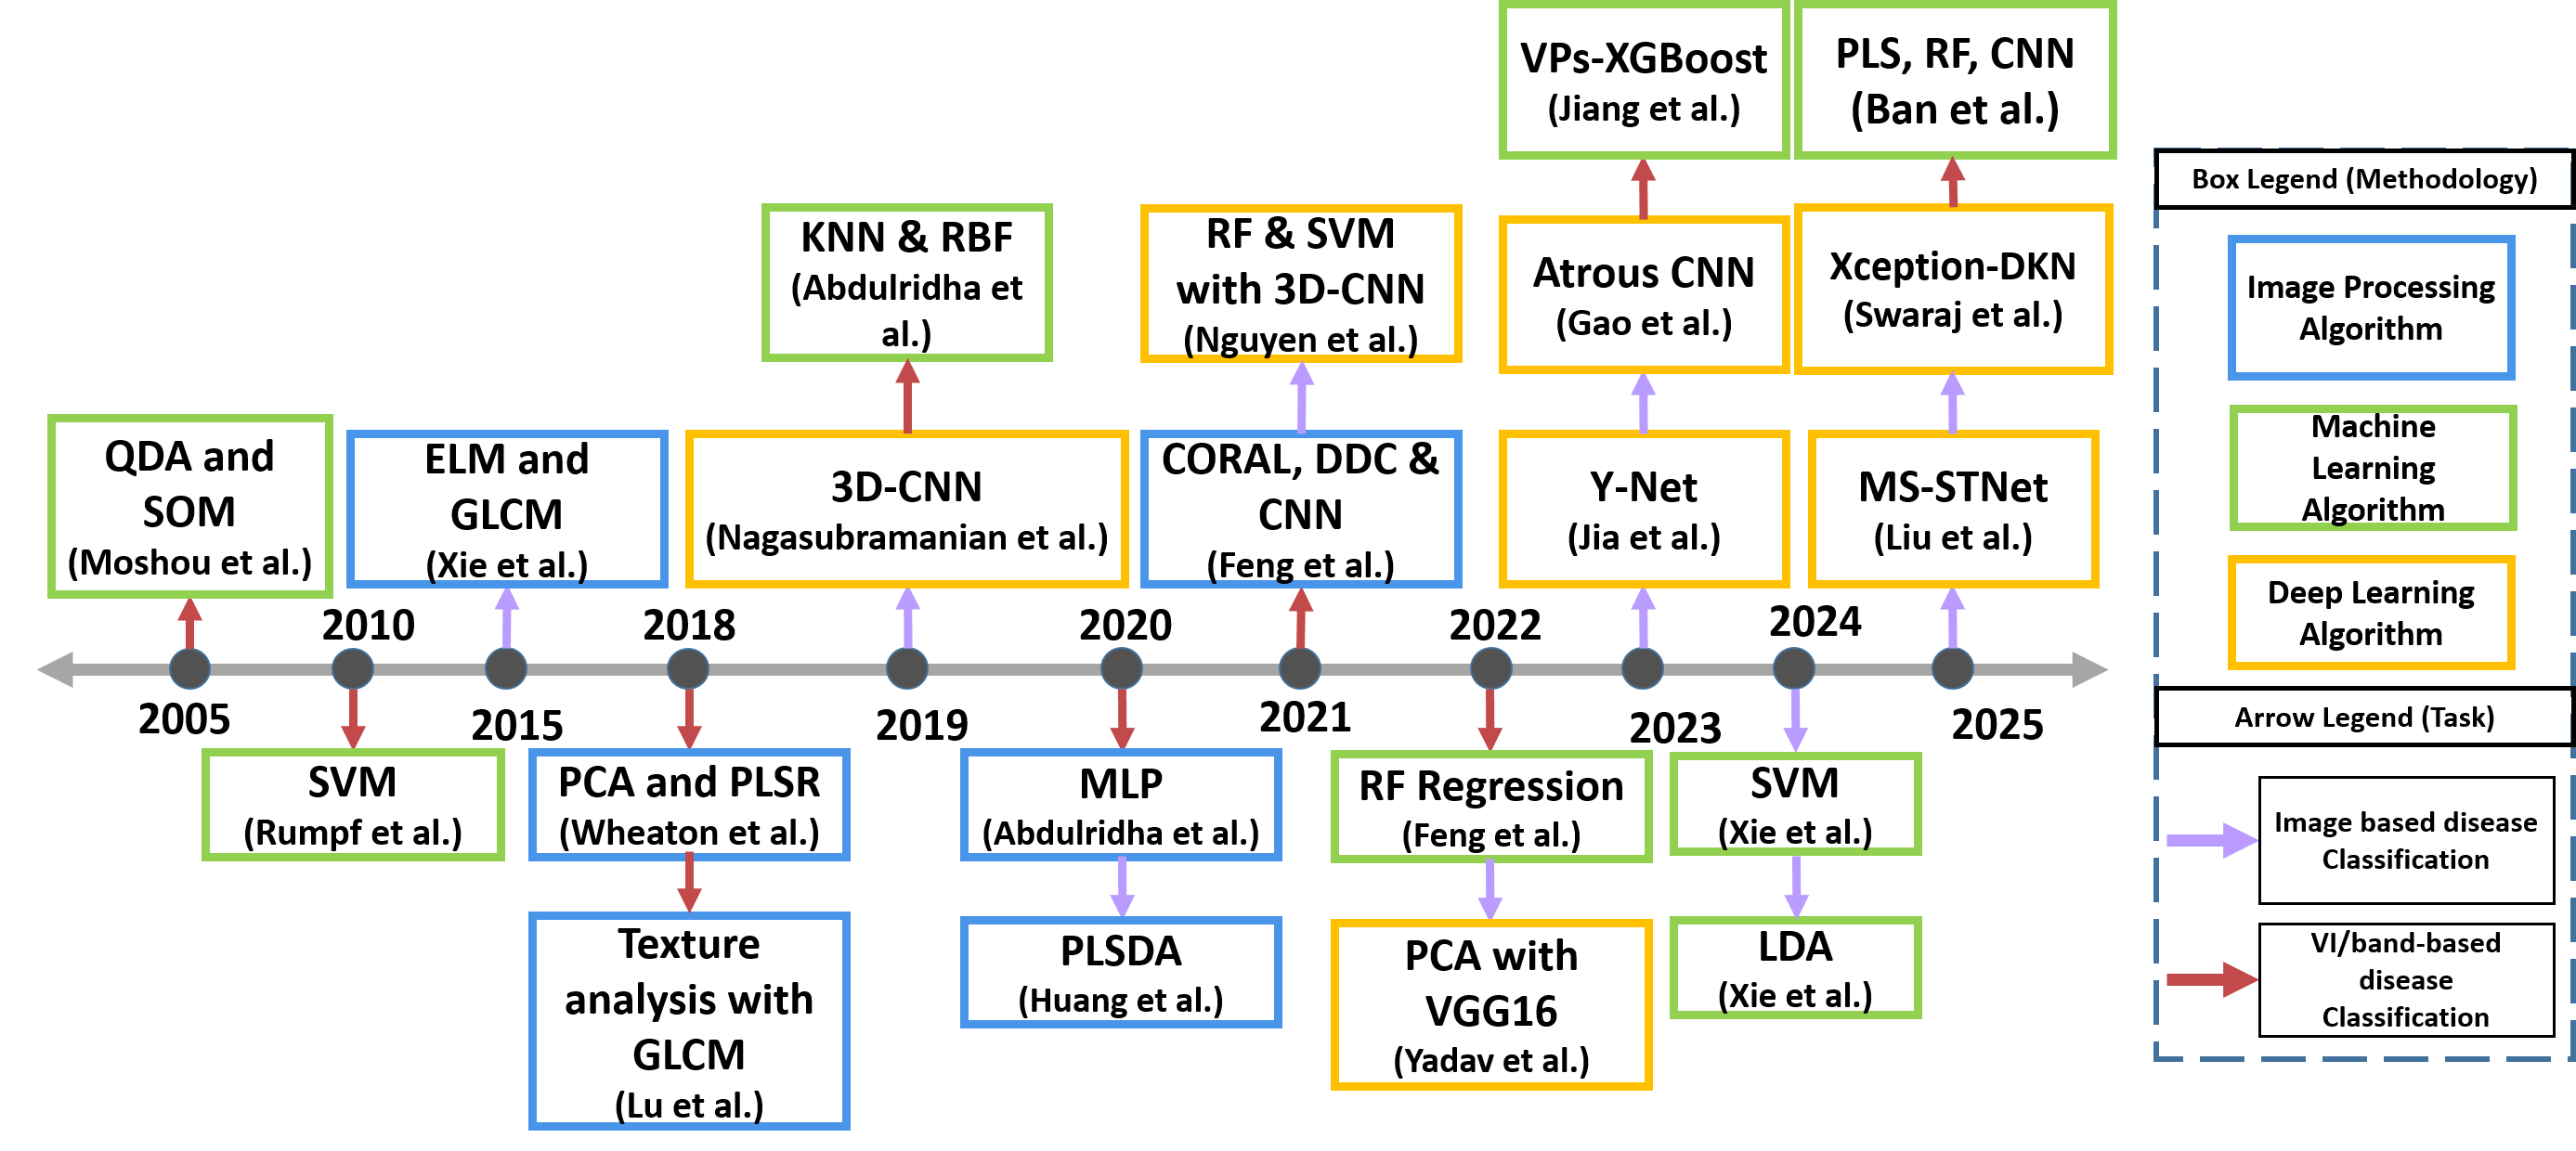
\includegraphics[width=1\textwidth]{Figure_10.png}
    \caption{Chronological overview of the most relevant methodologies for Plant Disease Detection using HSI. The color of the box represents the classification of methodology while the color of the arrow shows the task performed}
    \label{fig:timelineHSI}
\end{figure*}

The timeline reveals three distinct developmental phases: classical approaches (2005-2015) utilizing fundamental algorithms such as QDA \citep{MOSHOU200575}, SOM, and texture analysis with GLCM \citep{lu2018using}; machine learning integration (2015-2022) implementing SVM \citep{alisaac2018hyperspectral,cheshkova2023application,rumpf2010early}, RF regression \citep{feng2022hyperspectral,jiang2023monitoring}, and early CNN architectures \citep{liu2020disease,nagasubramanian2019plant}; and contemporary deep learning adoption (2022-2025) featuring sophisticated networks including Y-Net \citep{jia2023net}, MS-STNet \citep{liu2025early}, and Xception-DKN \citep{swaraj2025xception}.

This progression demonstrates increasing algorithmic sophistication across methodological generations, with recent developments incorporating multi-camera systems, biochemical parameter integration, and attention mechanisms. The evolution from simple classification approaches to complex multi-algorithm frameworks reflects the field's advancement toward more sophisticated pattern recognition capabilities while highlighting the continuous pursuit of improved accuracy and analytical depth in hyperspectral disease detection applications.

%%%%%%%%%%%%%%%%%%%%%%%%%%%%%%%%%%%%%%%%%%%%%%%%%%%%%

\section{Benchmarking Analysis} \label{sec:bm}

This section provides systematic comparative evaluation of state-of-the-art deep learning architectures across multiple plant disease datasets, addressing critical concerns regarding standardized performance assessment, reproducibility, and trade-off analysis between model complexity, generalization capabilities, and real-world applicability. Our benchmarking framework enables direct comparison of architectural capabilities across diverse agricultural scenarios, from controlled laboratory conditions to challenging field environments.

\subsection{Experimental Design and Reproducibility Framework}

Our evaluation encompasses both literature synthesis and exploratory analysis across datasets representing the laboratory-to-field complexity spectrum: PlantVillage (controlled laboratory conditions), PlantDoc and Cropped PlantDoc (mixed laboratory-field conditions), FieldPlant (natural field conditions), and Cassava Leaf Disease (crowd-sourced real-world imagery). The architectural selection spans traditional CNNs (ResNet50), modern CNNs (ConvNeXt), pure attention mechanisms (Vision Transformer), and hybrid approaches (SWIN Transformer).



\subsection{Classification Performance Analysis}

Table \ref{tab:classification_performance} reveals systematic performance patterns across environmental complexity levels with implications for agricultural deployment. 


\begin{table*}[h!]
  \tiny
  \centering
\caption{Classification performance comparison across plant disease datasets. Results are reported as Accuracy/F1-Score. Bold values indicate the best performance for each dataset, while italicized values denote the best result from the Exploratory Analysis. Reported values are means; corresponding statistical analysis is provided in Table~\ref{tab:statistical_analysis}. A dash (-) indicates unavailable or unreported results.}

  \label{tab:classification_performance}
  \begin{tabular}{@{}p{2cm}p{1.5cm}p{1.2cm}p{1.2cm}p{1.2cm}p{1.2cm}p{1.2cm}@{}}
    \toprule
    \textbf{Reference} & \textbf{Architecture} & \textbf{PV} & \textbf{PD} & \textbf{cPD} & \textbf{FP} & \textbf{CLD} \\
    \midrule 
    \citet{bruno2022improving} & EfficientNet-b7 & \textbf{99.99/0.99} & - & - & - & - \\
    \citet{schuler2022color} & Two-Branch DCNN & 99.48/0.9923 & - & - & - & - \\
    \citet{singh2020plantdoc} & GoogleNet & 99.35/0.9934 & - & - & - & - \\
    \citet{toda2019convolutional} & Inception V3 & 97.1/0.972 & - & - & - & - \\
    \citet{geetharamani2019identification} & 9-layer CNN & 99.46/0.9815 & - & - & - & - \\
    \citet{yu2023inception} & Inception Conv ViT & 99.94/0.9989 & 77.54/0.7723 & - & - & - \\
    \citet{wang2021t} & Tri-Linear CNN & 99.99/0.9999 & \textbf{85.8/0.85} & - & - & - \\
    \citet{chai2025plantaim} & PlantAIM & 99.66/0.9966 & - & - & - & - \\
    \citet{singh2019plant} & Inception ResNet-V2 & - & - & 70.53/0.70 & - & - \\
    \citet{singh2019plant} & VGG-16 & - & - & 44.52/0.44 & - & - \\
    \citet{wang2022dhbp} & Dual-stream HBP & 98.91/- & 75.06/- & - & - & - \\
    \citet{moupojou2023fieldplant} & MobileNet & - & - & \textbf{73.86}/- & 82.90/- & - \\
    \citet{moupojou2023fieldplant} & Inception ResNet V2 & - & - & - & 81.81/- & - \\
    \citet{moupojou2023fieldplant} & Inception V3 & - & - & - & 82.54/- & - \\
    \citet{zubair2025robust} & Ensemble CNN Model & 99.69/0.9719 & 60/0.53 & - & \textbf{83/0.8568} & - \\
    
    \citet{sambasivam2021predictive} & Custom CNN & - & - & - & - & 93.00/0.8426 \\
    \citet{zhong2022classification} & Transformer ResNet & - & - & - & - & 91.12/0.8426 \\
    \citet{zhuang2021deep} & ViT w/ K-Fold & - & - & - & - & 90.02/- \\
    \citet{ravi2022attention} & Attention Ensemble & - & - & - & - & 87.70/0.8660 \\
    \citet{maryum2021cassava} & UNET-EfficientNet & - & - & - & - & 89.08/- \\
    \citet{thai2023formerleaf} & Pruning ViT & - & - & - & - & \textbf{98.5/0.96} \\
    \citet{divya_cassava} & CIVE-SSL & - & - & - & - & 89.73/0.89 \\
    \citet{LI2025106981} & ITIMCA (VLM) & - & - & - & - & 78.00/0.79 \\
    \midrule 
    Exploratory Analysis & SWIN & 99.32/0.9931& \textit{77.63/0.7595}& \textit{88.07/0.8774}& 95.60/0.9547& \textit{88.00/0.87}\\
    Exploratory Analysis & ViT & 99.43/0.9943 & 76.42/0.7495& 86.17/85.79& \textit{96.00/0.96}& 85.90/0.8583\\
    Exploratory Analysis & ConvNeXt & \textit{99.47/0.9946}& 71.76/0.7046& 78.96/0.7859& 95.58/0.9568& 87.60/0.8767\\
    Exploratory Analysis & ResNet50 & 98.18/0.9818& 41.79/0.3437& 52.74/0.4806& 85.98/0.8386& 83.97/0.8403\\
    \bottomrule
  \end{tabular}
  
  \vspace{0.2cm}
  \footnotesize
  \textbf{Dataset Abbreviations:} PV - PlantVillage, PD - PlantDoc, cPD - Cropped PlantDoc, FP - FieldPlant, CLD - Cassava Leaf Disease Dataset
\end{table*}


Laboratory dataset performance (PlantVillage) shows convergence at 97-100\% accuracy across architectures, with minimal differentiation between approaches, as the 2.9 percentage point difference between Inception V3 (97.1\%) and EfficientNet-b7 (99.99\%) becomes negligible considering field deployment variations. Laboratory-to-field transitions reveal systematic performance degradation when moving to field datasets, with ConvNeXt declining 27.71 \% accuracy from laboratory conditions (99.47\% on PlantVillage) to field conditions (71.76\% on PlantDoc), and ResNet50 declining 56.39 percentage points (98.18\% on PlantVillage → 41.79\% on PlantDoc), inverting laboratory performance rankings. Architectural analysis indicates that hybrid approaches demonstrate superior field robustness, with SWIN achieving 88.07\% on field-collected Cropped PlantDoc dataset through combined convolutional and attention mechanisms, while pure attention mechanisms like ViT show greater environmental sensitivity despite laboratory advantages. Real-world deployment assessment reveals that field dataset FieldPlant maximum accuracy (96.00\% with ViT) exceeds the 90\% threshold for agricultural reliability, while field dataset Cassava performance variability (78-98.5\%) indicates inconsistent deployment suitability across architectures.


Table \ref{tab:detection_performance} demonstrates that spatial localization requirements significantly amplify deployment challenges beyond classification tasks. 

\begin{table}[h!]
  \small
  \centering
  \caption{Detection Performance Comparison on Plant Disease Datasets. Bold entries indicate best performance per dataset. Dash (-) indicates unreported values.}
  \label{tab:detection_performance}
  \begin{tabular}{@{}p{2.5cm}p{2cm}p{3.5cm}p{1.25cm}p{1.25cm}@{}}
    \toprule
    \textbf{Reference} & \textbf{Architecture} & \textbf{Backbone} & \textbf{PD (mAP)} & \textbf{FP (mAP)} \\
    \midrule
    \citet{ye2023cascade} & Cascade-DN-Def-DETR & ResNet50 & \textbf{63.90} & - \\
    \citet{li2022improved} & YOLOv5s & CSPDarknet & 63.90 & - \\
    \citet{liu2022improved} & YOLOX-ASSANano & BSConv & 58.86 & - \\
    \citet{singh2019plant} & Faster RCNN & Inception ResNet v2 & 38.9 & - \\
    \citet{zhang2022automatic} & Transvolution + GAN & Custom & 50.3 & - \\
    \citet{moupojou2023fieldplant} & Faster RCNN & Inception ResNet v2 & 58.0 & 14.0 \\
    \citet{moupojou2023fieldplant} & YOLOv8 & CSPDarknet & - & 10.2 \\
    \citet{moupojou2023fieldplant} & SSD & MobileNet v2 & - & \textbf{14.4} \\
    \bottomrule
  \end{tabular}
  
  \vspace{0.2cm}
  \footnotesize
  \textbf{Dataset Abbreviations:} PD - PlantDoc, FP - FieldPlant
\end{table}


Task complexity analysis reveals that simultaneous classification and localization creates compound performance degradation, with field dataset PlantDoc detection achieving 63.9\% mAP compared to 85.8\% classification accuracy, representing a 21.9 percentage point reduction when spatial requirements are added. Field environment assessment shows that FieldPlant detection performance (10.2-14.4\% mAP) falls substantially below research utility thresholds, indicating fundamental limitations in complex agricultural environments across all architectural approaches tested.

\subsection{Comparative Analysis of Plant Disease Detection Approaches}

To address the need for systematic comparison across deployment-critical dimensions, Table \ref{tab:technique_comparison} provides comprehensive evaluation of major methodological approaches across cost, speed, accuracy, scalability, and field usability criteria. This analysis combines insights from recent literature and current market data to guide practical deployment decisions.
\begin{table*}[h!]
\centering
\tiny
\caption{Comparative Analysis of Plant Disease Detection Techniques Across Deployment Dimensions}
\label{tab:technique_comparison}
\begin{tabular}{@{}p{4.5cm}p{1.5cm}p{1.5cm}p{2cm}p{1.5cm}@{}}
\toprule
\textbf{Technique Category} & \textbf{Hardware Cost} & \textbf{Processing Speed} & \textbf{Field Accuracy} & \textbf{Scalability} \\
\midrule
\multicolumn{5}{c}{\textbf{RGB-Based Approaches}} \\
\midrule
Classical RGB (Color analysis, GLCM) & USD50-300 \citep{coptrz2024cost} & Real-time \citep{straits2022hsi} & 60-75\% \citep{arivazhagan2013detection} & High \\
RGB + ML (SVM, Random Forest) & USD200-800 \citep{coptrz2024cost} & Near real-time \citep{hatuwal2020plant} & 70-85\% \citep{qin2016identification} & High \\
RGB + Deep Learning (CNN, ResNet, ViT) & USD800-3000 \citep{coptrz2024cost} & 0.2-1 sec/image \citep{Viel2023time} & 75-90\% \citep{ferentinos2018deep} & Moderate \\
RGB + Vision-Language (CLIP, GPT-4V) & USD1500-5000 \citep{coptrz2024cost} & 5-30 sec/image \citep{zhang2024visual} & 70-85\% \citep{LI2025106981} & Low \\
\midrule
\multicolumn{5}{c}{\textbf{Hyperspectral Approaches}} \\
\midrule
HSI + Classical (Spectral indices, PCA) & USD15K-60K \citep{sph2024hyperspectral} & 1-60 sec \citep{GhamisiHSI} & 80-95\% \citep{abdulridha2020detection} & Low \\
HSI + ML (SVM, PLS regression) & USD20K-75K \citep{sph2024hyperspectral} & 1-5 min \citep{Viel2023time} & 85-95\% \citep{alisaac2018hyperspectral} & Low \\
HSI + Deep Learning (1D to 3D-CNN, Spectral Nets) & USD30K-100K \citep{sph2024hyperspectral} & 1-20 min \citep{Viel2023time,detring2024quality} & 90-98\% \citep{jia2023net} & Very Low \\
\midrule
\multicolumn{5}{c}{\textbf{Multimodal Approaches}} \\
\midrule
RGB + Multispectral (4-8 bands) & USD3K-12K \citep{advexure2025multispectral} & 2-10 sec \citep{coptrz2024multispectral} & 80-92\% \citep{cao2018fast} & Moderate \\
RGB + Environmental (Weather, soil sensors) & USD500-2000 \citep{coptrz2024cost} & Real-time \citep{das2024machine} & 75-88\% \citep{khan2025integration} & High \\
UAV Systems (RGB/Multispectral) & USD5K-30K \citep{advexure2025mavic,coptrz2024multispectral} & Field-dependent \citep{gano2024drone} & 67-85\% \citep{garcia2019comparison} & High \\
\midrule
\multicolumn{5}{c}{\textbf{Mobile/Edge Solutions}} \\
\midrule
Smartphone Apps (Plantix, PlantNet) & USD100-1,000 \citep{coptrz2024cost} & 0.5-3 sec \citep{rani2023role} & 65-80\% \citep{strey2022plantix} & Very High \\
Edge AI Devices (Jetson, Coral) & USD250-2000 \citep{nvidia2024jetson,nvidia2024orin} & 0.02-2 sec \citep{mahmud2024light} & 70-85\% \citep{mahmud2024light} & High \\
IoT Sensor Networks (Distributed monitoring) & USD200-1000/node \citep{dfi2024edge} & Continuous \citep{nvidia2024edge} & 60-80\% \citep{neupane2021automatic} & Very High \\
\bottomrule
\end{tabular}
\end{table*}

The comparative analysis reveals distinct deployment trade-offs across methodological approaches:

\begin{itemize}
    \item [--]\textbf{Cost-accuracy relationships} demonstrate a clear stratification: smartphone applications offer optimal cost-performance ratios for widespread deployment, hyperspectral approaches achieve superior accuracy (90-98\%) at substantially higher costs (USD30K-100K), while classical RGB methods provide intermediate solutions for resource-constrained scenarios.
    
    \item [--] \textbf{Processing speed analysis} reveals an inverse correlation with accuracy, where real-time approaches (RGB classical, IoT sensors) sacrifice precision for deployment speed, whereas high-accuracy hyperspectral methods require processing times (1-20 minutes) that challenge real-time agricultural decision-making \citep{Viel2023time, detring2024quality}. This extended processing time primarily stems from extensive data preprocessing requirements including quality assurance, calibration, and spectral normalization, with deep learning inference representing only 1-2 minutes of the total pipeline.
    
    \item [--] \textbf{Scalability assessment} indicates technological sophistication inversely correlates with deployment potential. The simpler approaches demonstrate excellent scalability characteristics, while advanced methods face computational, expertise, and infrastructure limitations.
    
    \item [--] \textbf{Field deployment readiness} varies significantly: RGB-based solutions demonstrate immediate deployment capability with minimal technical requirements, hyperspectral approaches remain primarily research-focused requiring controlled conditions, and multimodal solutions occupy an intermediate position requiring targeted implementation strategies. Architectures like MobileNet, achieving comparable accuracy of 82.5\% \citep{moupojou2023fieldplant}, exemplify this readiness through 4.2MB model sizes and 22ms inference times on mobile devices, enabling direct deployment without specialized infrastructure.
    \end{itemize}

The analysis suggests a technology readiness spectrum from mature smartphone-based solutions to emerging hyperspectral and multimodal approaches, guiding selection based on deployment constraints, accuracy requirements, and operational contexts.

\section{Practical Deployment Case Studies} \label{sec:practical_deployment}
This section examines documented real-world applications of deep learning models for plant disease detection, highlighting achievements and success rates in operational environments.

\subsection{Commercial and CGIAR Platform Deployments}

\subsubsection{Plantix: Commercial Success Model}

Plantix represents one of the most successful commercial deployments of AI-driven plant disease detection, with over 10 million downloads across 60+ countries \citep{strey2022plantix, peat2020plantix}. The platform maintains 1 million monthly active users, processing approximately 20,000 image uploads daily \citep{harvard2022plantix}. Machine learning algorithms identify over 385 crop diseases across 30+ crops, achieving detection accuracy over 90\% for most classes \citep{samal2018automated}. However, real-world deployment revealed connectivity challenges in rural areas and the need for continuous model updates across diverse environmental conditions \citep{acs2019plantix}.

\subsubsection{CGIAR Innovation Ecosystem}

CGIAR (Consultative Group for International Agricultural Research) is a global research partnership dedicated to reducing poverty, enhancing food security, and improving natural resources management in developing countries through 15 research centers that develop science-based solutions for smallholder farmers.

\textbf{Tumaini for Banana and Bean Disease Detection:} Developed by the Alliance of Bioversity International and CIAT under the CGIAR Research Program on Roots, Tubers and Bananas (RTB), Tumaini demonstrates successful deep learning translation to practical smallholder-focused tools for banana and common bean disease management. With over 14,000 downloads and 70-99\% success rates depending on plant parts and diseases detected \citep{tumaini2024bioversity}, the app evolved from banana-specific detection to the October 2024 launch of Tumaini Beans, directly addressing smallholder farmer needs for both banana and common bean disease management. Key accessibility features include offline functionality, multilingual support in five languages, and broad Android compatibility.

\textbf{PlantVillage Nuru for Cassava and Potato:} This collaborative CGIAR initiative developed by Penn State University with IITA, FAO, and CIMMYT utilizes CNNs through TensorFlow to enable offline cassava disease diagnosis, achieving twice the accuracy of agricultural extension workers \citep{legg2020nuru}. The platform expanded to potato disease detection in 2021, serving over two million farmers in East Africa \citep{hughes2021potato}, with future plans including sweet potato, yams, and banana integration.

\textbf{Integrated Agricultural Decision Support:} Akilimo (IITA) provides comprehensive decision support extending beyond disease detection to fertilizer optimization and crop management \citep{iita2021akilimo}. ICRISAT's Sowing app resulted in farmers achieving 30\% yield increases \citep{icrisat2024digital}, while AfricaRice's RiceAdvice achieved significant smallholder adoption \citep{africarice2024riceadvice}, demonstrating effective AI integration with agricultural extension systems.



\subsection{CGIAR Digital Integration Framework}

The CGIAR Platform for Big Data in Agriculture provides foundational infrastructure for integrating deep learning disease detection models into existing agricultural decision support systems \citep{cgiar2020bigdata}. This platform democratizes decades of agricultural data, enabling integration of disease detection algorithms with comprehensive datasets spanning multiple crops, regions, and farming systems.

Figure \ref{fig:cgiar_pipeline} illustrates the systematic integration pipeline for translating deep learning research into practical smallholder applications. The framework demonstrates a five-step process from model development to deployment, with CGIAR Centers providing continuous support through research coordination, field networks, technical expertise, and partnership management. A feedback loop ensures continuous model refinement based on field data collection, creating sustainable improvement cycles for disease detection algorithms.

\begin{figure}
    \centering
    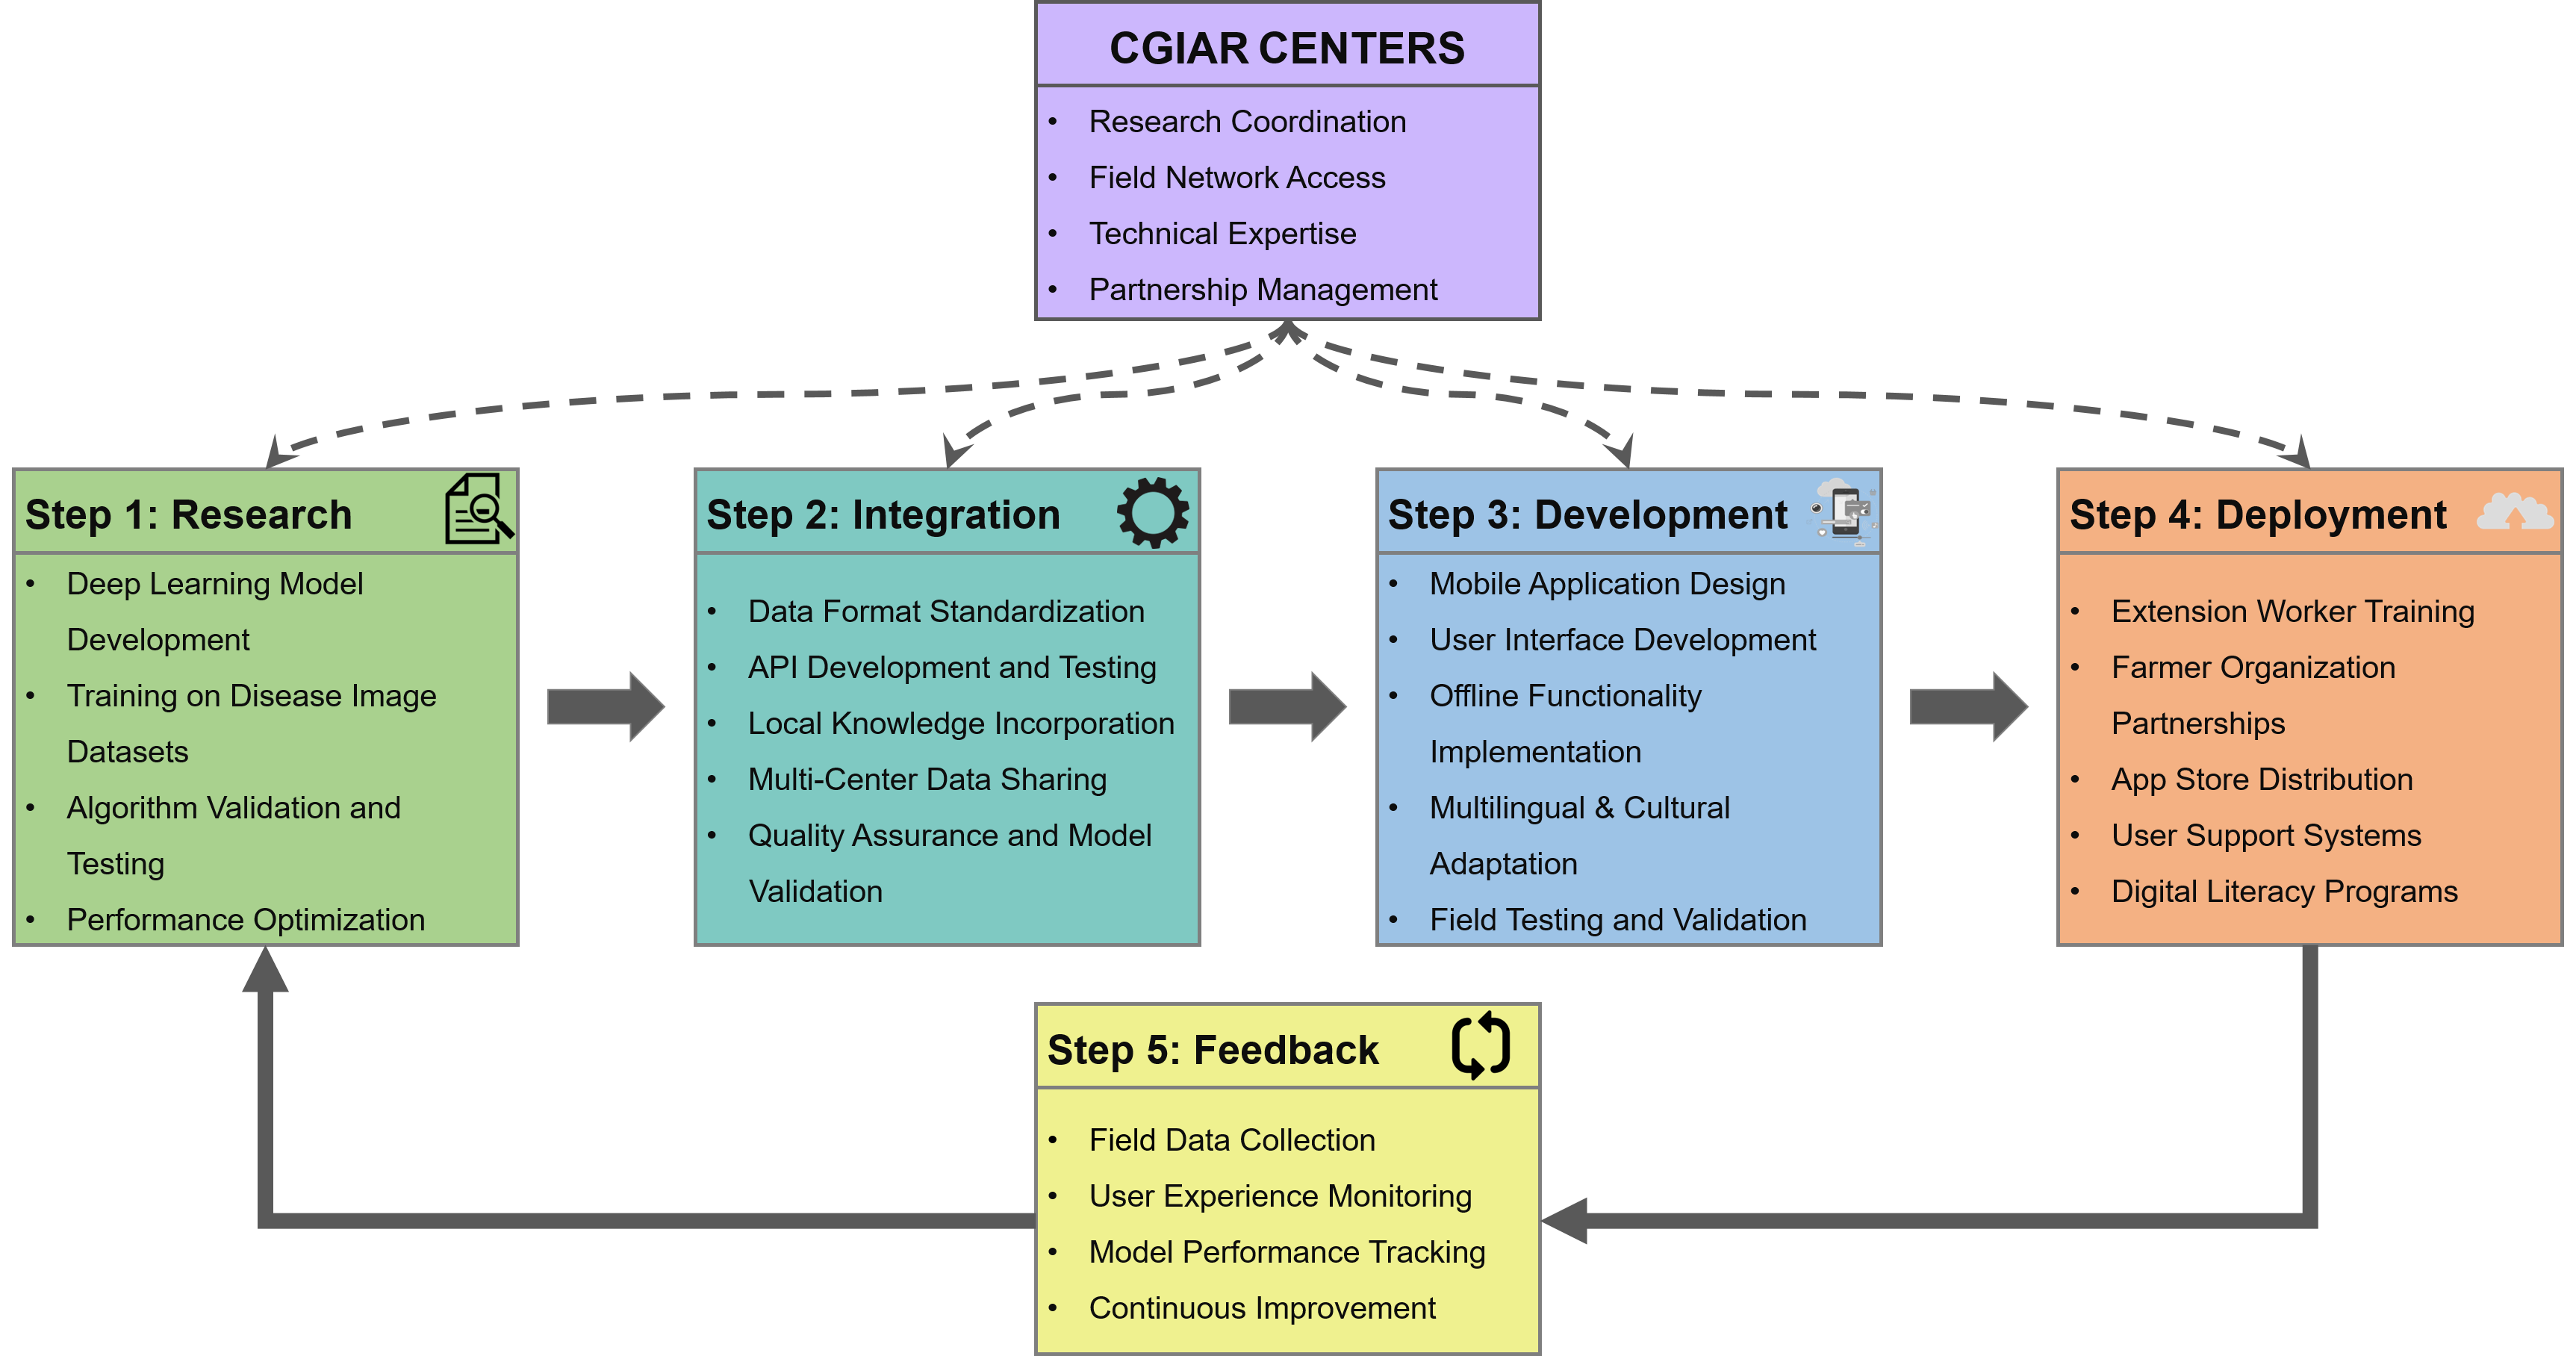
\includegraphics[width=1.0\linewidth]{Figure_11.png}
    \caption{Deep learning integration pipeline for plant disease detection through CGIAR infrastructure, showing systematic progression from research development to smallholder farmer deployment with continuous feedback mechanisms.}
    \label{fig:cgiar_pipeline}
\end{figure}

Integration occurs through systematic approaches ensuring practical smallholder implementation:
\begin{itemize}
    \item [--] \textbf{Standardized APIs}: Technical interfaces that allow deep learning disease detection models developed by researchers to communicate directly with existing CGIAR mobile applications and web platforms, eliminating the need to rebuild entire systems and enabling rapid deployment of new detection capabilities to farmers already using CGIAR tools.
    
    \item [--] \textbf{Data Standards Compatibility}: Research models are adapted to work with the established data collection formats, image specifications, and reporting protocols already used across CGIAR's global network, ensuring that new disease detection algorithms can seamlessly process existing agricultural datasets and farmer-submitted images without requiring additional technical training.
    
    \item [--] \textbf{Farmer Database Integration}: Disease detection algorithms connect with existing farmer registration systems and agricultural databases maintained by CGIAR centers, enabling personalized disease management recommendations based on individual farm characteristics, cropping history, local climate conditions, and previously reported disease incidents.
    
    \item [--] \textbf{Local Knowledge Incorporation}: Traditional agricultural practices, indigenous crop varieties, and farmer-generated knowledge about local disease patterns are systematically integrated into deep learning models through CGIAR's extensive field networks and agricultural extension partnerships, ensuring that AI recommendations complement rather than replace proven local farming wisdom.
    
    \item [--] \textbf{National Research Partnerships}: Established collaborative relationships between CGIAR centers and national agricultural research institutions provide validated pathways for deploying disease detection tools across diverse farming environments, climatic zones, and regulatory frameworks, with local partners ensuring cultural appropriateness and regulatory compliance.
    
    \item [--] \textbf{Smallholder-Focused Validation}: All integration processes prioritize accessibility for resource-constrained farmers through features like offline functionality, low-bandwidth image processing, multilingual interfaces, compatibility with basic smartphones, and integration with existing farmer support networks rather than requiring new infrastructure investments.
\end{itemize}

\subsection{UAV-Based Disease Detection and Surveillance Systems}

Unmanned Aerial Vehicle (UAV) platforms have emerged as transformative tools for large-scale crop disease surveillance, enabling comprehensive monitoring of agricultural landscapes through high-resolution aerial imaging and advanced deep learning architectures. These systems address the limitations of ground-based detection methods by providing broader spatial coverage, reduced labor requirements, and enhanced accessibility to remote or difficult-to-reach agricultural areas, particularly addressing scalability challenges for large-scale monitoring in smallholder farming systems.

\textbf{Advanced Deep Learning Applications:} Recent developments demonstrate sophisticated integration of UAV platforms with state-of-the-art deep learning models. \citet{selvaraj2020detection} developed a mixed-model system combining RetinaNet object detection with custom classifiers for simultaneous banana localization and disease classification using UAV-RGB imagery, achieving 99.4\%, 92.8\%, 93.3\%, and 90.8\% accuracy for banana bunchy top disease (BBTD), Xanthomonas Wilt of Banana (BXW), healthy banana clusters, and individual plants respectively, while demonstrating multi-platform integration across satellite (Sentinel-2, PlanetScope, WorldView-2) and UAV (MicaSense RedEdge) systems with random forest models achieving 97\% overall accuracy for banana classification in mixed-complex African landscapes. 

\citet{mora2025digital} developed a georeferenced multiplatform surveillance system integrating UAV-based aerial imaging with ground-level detection using YOLO foundation models (YOLO-NAS, YOLOv8, YOLOv9) and Faster-RCNN for banana wilt identification, with YOLOv9 achieving superior performance in UAV aerial images (55-86\% mAP@50) and YOLOv8 excelling in ground-level detection (65-99\% mAP@50) across global datasets from Africa, Latin America, India, Asia, and Australia, while incorporating explainable AI techniques including Gradient-weighted Class Activation Mapping and Human-in-the-Loop AI for enhanced model transparency and prediction refinement. \citet{mora2024pixels} implemented UAV-enabled transfer learning approaches using YOLOv8 and Faster R-CNN for BXW detection in African smallholder systems, utilizing pansharpening algorithms for improved RGB and multispectral data fusion from unmanned aerial vehicles and achieving 75-99\% detection accuracy across precision, recall, and F1 metrics, demonstrating the effectiveness of cutting-edge deep learning architectures for crop health assessment in complex agricultural landscapes targeting food security applications.

\textbf{Cost-Effective and Commercial Solutions:} University of New Hampshire researchers have developed cost-effective UAV solutions specifically designed for smaller farms, using fewer multispectral bands to reduce costs while maintaining effectiveness for early disease detection \citep{unh2024drones}. The Flyix AI platform demonstrates commercial viability by reducing annotation time by 99.7\%, enabling real-time disease analysis through large-scale aerial imagery processing \citep{flypix2025crop}.

\textbf{Implementation Challenges and CGIAR Integration:} However, UAV-based detection faces persistent challenges from spectral reflectance variations, environmental factors, image distance, occlusion, and illumination conditions \citep{mdpi2023drones, springer2023precision, frontiers2022drone}. Integration with CGIAR field networks could provide validation frameworks for UAV-based disease detection systems supporting banana and common bean monitoring in smallholder farming systems, leveraging established agricultural networks to address these technical challenges while ensuring practical deployment in resource-constrained environments.

\subsection{Critical Success Factors}

Analysis of successful deep learning implementations reveals essential factors for effective translation from research to practical smallholder agriculture applications. Several validated deployments demonstrate these principles in action: the mobile-enabled Plant Diagnosis Application achieved 93.91\% accuracy for Sub-Saharan Africa agricultural challenges through community-centered design and offline functionality \citep{frontiers2023mpd}, a habanero-specific application using Modified VGG16 achieved 98.79\% accuracy by focusing on crop-specific optimization \citep{nature2024habanero}, while DeepCrop utilizing ResNet50 achieved 98.98\% accuracy and successful real-life web deployment through scalable architecture design \citep{sciencedirect2023deepcrop}.
These successful implementations highlight critical success factors including community integration through partnerships with agricultural universities, multilingual adaptation for global accessibility, offline functionality for remote areas, and integration with national extension systems. CGIAR's established relationships with Farmer Producer Organizations enhance service delivery and scaling, while platform integration reduces development costs and provides comprehensive agricultural support through established channels, particularly benefiting smallholder farmers managing banana and common bean diseases in resource-constrained environments across low- and middle-income countries.

%%%%%%%%%%%%%%%%%%%
\par The practical deployment experiences reveal both significant achievements and persistent challenges in translating deep learning advances into real-world agricultural settings. While platforms like Plantix, Tumaini, and Nuru demonstrate successful CNN implementation, infrastructure limitations, economic constraints, and environmental variability continue restricting widespread adoption. CGIAR's digital agriculture ecosystem represents a proven pathway for translating research advances into scalable solutions directly benefiting smallholder farmers, particularly for banana and common bean disease detection in low- and middle-income countries.

\section{Future Research Directions and Research Priorities} \label{sec:frd}
This systematic review identifies significant gaps between laboratory performance and field implementation across methodological approaches in plant disease detection. Analysis of performance-cost relationships presented in Table \ref{tab:technique_comparison} and benchmarking results in Table \ref{tab:classification_performance} reveals research priorities that emphasize deployment feasibility alongside technical advancement. The observed 15-30\% performance reduction from laboratory to field conditions across different architectures indicates the need for research approaches that prioritize practical implementation considerations.


\subsection{Performance and Deployment Considerations}

Comparative analysis reveals patterns that influence agricultural deployment success. Computational efficiency analysis presented in Table \ref{tab:computational_complexity} indicates that advanced architectures such as Vision Transformers (85.8M parameters) and ConvNeXt (87.6M parameters) provide incremental accuracy improvements while requiring substantial computational resources. ResNet50 demonstrates higher efficiency ratios (23.96 throughput per million parameters) compared to transformer-based approaches (SWIN: 1.47), suggesting that deployment optimization may benefit from architectural efficiency rather than increased complexity. Performance evaluation across different datasets reveals environmental adaptation challenges, with models such as ConvNeXt showing accuracy variations from 99.47\% on controlled datasets (PlantVillage) to 71.76\% on field-collected data (PlantDoc), representing a 27.71\% performance difference. This pattern occurs consistently across architectures, indicating systematic challenges in environmental adaptation that extend beyond individual model limitations and suggest fundamental considerations for field deployment strategies.

\subsection{Implementation-Oriented Architecture Development}
Current research typically prioritizes laboratory accuracy optimization before addressing deployment requirements. Future research approaches should integrate implementation considerations into the design process from initial development stages. Resource-efficient optimization represents a key research area, focusing on architectures that achieve model sizes under 5MB with inference times below 100ms while maintaining field accuracy above 80\%. Analysis of successful mobile applications such as Plantix, which has achieved adoption by over 10 million users, demonstrates that accessibility and usability often determine deployment success more than technical sophistication, suggesting that constraint optimization may enhance practical viability. Adaptive complexity systems present another research opportunity, involving the development of models that dynamically adjust computational requirements based on available hardware resources. This approach would enable deployment across diverse infrastructure contexts, from edge devices (USD250-2,000) to high-performance systems (USD5,000-30,000) as detailed in Table \ref{tab:technique_comparison}. Economic viability assessment should be integrated into evaluation frameworks alongside traditional technical metrics. Case study analysis indicates that successful platforms prioritize user accessibility and cost-effectiveness over peak accuracy performance, suggesting that economic considerations should inform architectural design decisions to enhance real-world adoption and implementation success.

\subsection{Geographic Generalization Through Distributed Learning Approaches}
Agricultural AI systems demonstrate performance variations of 40-60\% across different climate zones, indicating opportunities for improved generalization methodologies. Federated learning approaches represent a promising research direction for agricultural applications, enabling collaborative model training while maintaining data privacy and respecting regional data governance requirements. Such distributed learning architectures could potentially reduce performance variation across diverse geographic contexts to below 10\% through shared knowledge while preserving local data sovereignty.

Few-shot learning frameworks offer another avenue for geographic adaptation, focusing on meta-learning systems that enable rapid model adaptation to new environmental contexts using minimal local training data (under 100 samples). Analysis of architectural performance indicates that transformer-based approaches such as Vision Transformers achieve higher accuracy on field datasets (96.00\% on FieldPlant) compared to convolutional neural networks like ResNet50 (85.98\%), suggesting potential advantages for adaptation tasks. 

Climate-aware domain adaptation presents an additional research opportunity, involving the integration of environmental variables that influence disease manifestation and spectral characteristics into model architectures. This approach could address the temporal and geographic sensitivity observed in current detection systems by explicitly modeling environmental factors that affect disease presentation across different agricultural regions and seasons.

\subsection{Interpretable Multimodal System Development}
Agricultural technology adoption requires decision-making systems that balance technical capabilities with user comprehension and practical implementation needs. Cost-effective detection frameworks represent a significant research opportunity, involving progressive systems that utilize RGB imaging for initial screening purposes (USD50-3,000) followed by targeted hyperspectral confirmation where necessary (USD15,000-100,000). This staged approach could potentially reduce per-sample analysis costs by 70-80\% while preserving diagnostic accuracy by leveraging the complementary advantages of different imaging modalities as demonstrated in Table \ref{tab:technique_comparison}. Attention-based explainability mechanisms present another important research direction, focusing on architectures that provide visual interpretations of diagnostic reasoning processes. Analysis indicates that agricultural practitioner adoption depends significantly on transparent decision-making capabilities, suggesting the need for systems that integrate technical accuracy with interpretable outputs that enable informed user decision-making. Temporal monitoring systems offer additional research potential through approaches that track disease progression over time rather than providing single-point detection results. Such longitudinal monitoring capabilities could enable precision intervention strategies by incorporating predictive disease modeling that informs optimal timing and targeting of treatment applications, potentially improving both agricultural outcomes and resource efficiency in disease management practices.



\subsection{Field-Based Evaluation Framework Development}
Current evaluation methodologies using curated laboratory datasets may not accurately reflect operational performance characteristics in agricultural settings. Establishing standardized evaluation protocols based on field-collected datasets represents an important research priority for validating system performance under operational conditions across diverse geographic regions. Analysis indicates substantial performance differences between laboratory datasets such as PlantVillage (97-99\% accuracy) and field-collected datasets like PlantDoc (41-85\% accuracy), suggesting that evaluation frameworks should incorporate real-world data collection conditions to provide more accurate performance predictions for deployment scenarios. User-centered evaluation approaches present another methodological development opportunity, involving the integration of practitioner experience factors such as user interface usability, decision confidence measures, and adoption willingness alongside traditional technical performance metrics. This comprehensive evaluation approach would provide a more complete assessment of system viability for agricultural implementation by considering both technical capabilities and human factors that influence successful technology adoption in operational agricultural contexts.


\subsection{Responsible AI Development for Agricultural Applications}
Ethical considerations in agricultural AI development require systematic approaches to ensure equitable and responsible technology deployment. Bias detection and mitigation methodologies represent a critical research area, focusing on developing techniques to identify potential dataset biases that may disadvantage specific crop varieties, farming systems, or geographic regions. Analysis reveals representation gaps across geographic and socioeconomic contexts in current datasets, indicating the need for more inclusive data collection and model development practices. Impact assessment frameworks for diagnostic errors present another important research direction, involving the quantification of agricultural and economic consequences associated with false positive results (leading to unnecessary treatments) and false negative outcomes (allowing unchecked disease progression) across different farming contexts and scales. Understanding these impact patterns is essential for developing appropriate decision thresholds and risk management strategies. Technology accessibility research offers additional opportunities to address equity considerations in agricultural AI deployment. This includes developing strategies that ensure smallholder farming operations have access to technological capabilities comparable to those available for industrial-scale operations, addressing the digital divide identified in cost analysis studies. Such approaches could involve scalable deployment models, cooperative technology sharing frameworks, and development of cost-effective solutions specifically designed for resource-constrained agricultural contexts.

%\subsection{Implementation Roadmap}

%\textbf{Phase 1 (2025-2026): Foundation Development}
%Establish field-validated benchmarks across 5+ climate zones; deploy lightweight prototypes achieving >75\% field accuracy; develop economic impact assessment frameworks integrating cost-benefit analysis.

%\textbf{Phase 2 (2027-2029): Scale and Integration}
%Deploy federated learning networks across 100+ agricultural sites; implement multimodal fusion systems reducing costs by 60\% while maintaining performance; establish farmer training programs ensuring technology adoption.

%\textbf{Phase 3 (2030+): Agricultural Transformation}
%Scale to 10,000+ farms across developing and developed regions; integrate with automated intervention systems for closed-loop disease management; demonstrate measurable impact on global food security metrics.

\subsection{Collaborative Research Framework}
Advancing agricultural disease detection requires interdisciplinary collaboration, integrating expertise from computer science, plant pathology, agricultural economics, and farming communities. Partnerships between researchers and practitioners are essential to ensure that end-user needs inform technology development from design to deployment. Addressing adoption barriers identified in deployment studies depends on incorporating these perspectives early in the research cycle. Open-source initiatives further support reproducibility, knowledge exchange, and broader validation by providing shared models, datasets, and evaluation protocols. Additionally, developing technology transfer infrastructure is critical for bridging the gap between research and practical application, enabling systematic evaluation and adaptation of detection technologies across diverse farming systems and regions.

The advancement of plant disease detection technologies from research environments to operational agricultural applications requires research approaches that integrate practical implementation considerations alongside technical development. These research directions provide frameworks for developing detection systems that can effectively contribute to agricultural productivity and food security objectives through successful field deployment and adoption.

\section{Conclusion} \label{sec:conclusion}

This systematic review examines the advancement of plant disease detection technologies from research environments to operational agricultural applications through comprehensive analysis of RGB and hyperspectral imaging approaches across methodological developments. The analysis reveals important considerations for bridging technical achievements with practical implementation requirements in agricultural contexts.


Our analysis identifies three critical patterns informing agricultural AI development. The performance-implementation relationship shows laboratory accuracies of 95-99\% across computational approaches contrasting with adoption challenges, reflecting differences between research optimization criteria and deployment requirements including environmental robustness, economic viability, and user interpretability. The observed 15-30\% performance variation during laboratory-to-field transitions indicates systematic implementation considerations beyond computational optimization. Technology accessibility trade-offs demonstrate that while hyperspectral imaging achieves superior laboratory detection through extended spectral range, associated costs (USD20,000-50,000 vs. USD500-2,000 for RGB), computational requirements, and expertise needs create accessibility barriers, explaining why RGB approaches achieve broader adoption despite spectral limitations. Methodological evolution analysis reveals progression from classical image processing through machine learning to deep learning, with emerging applications combining agricultural expertise with AI capabilities, providing foundations for systems that augment agricultural decision-making while addressing interpretability requirements.


Evaluation of 150+ studies identifies consistent deployment factors. Environmental adaptation challenges affect both RGB and HSI approaches under field conditions due to illumination variations, atmospheric factors, and canopy complexity differences from laboratory settings, persisting across methodological approaches and indicating systematic rather than technique-specific challenges. Economic viability analysis shows that advanced computational approaches present cost-performance relationships requiring consideration alongside technical capabilities, with agricultural budget constraints influencing technology selection and suggesting the importance of deployment-oriented design. Geographic generalization limitations reveal that models optimized for specific conditions show reduced performance across different temporal and geographic contexts, highlighting the importance of robust validation and adaptation strategies.


Benchmarking analysis establishes evidence-based deployment recommendations. Hybrid architectures such as SWIN Transformer demonstrate improved field performance (88.07\% vs. 52.74\% for traditional CNNs) through combined mechanisms, while performance expectations should target 80-87\% field accuracy rather than laboratory benchmarks of 97-100\%. Cost-effectiveness analysis indicates smartphone applications provide favorable ratios (USD100-1,000, 65-80\% accuracy) for broad deployment, while hyperspectral approaches achieve higher accuracy (90-98\%) at increased costs suitable for specialized applications.

Future advancement requires integrated approaches addressing technical performance and practical implementation through deployment-oriented development that considers economic feasibility, environmental robustness, and interpretability alongside optimization. Field-based validation protocols, interdisciplinary collaboration including farmer-researcher partnerships, and economic assessment frameworks measuring agricultural return on investment represent priority research directions. Plant disease detection technologies have reached a development stage where continued advancement requires balanced consideration of technical capabilities and practical agricultural utility, with future systems combining accessibility and interpretability essential for adoption with analytical capabilities necessary for effective disease management. The frameworks established provide guidance for developing agricultural AI systems that successfully bridge computational sophistication with practical application, contributing to both technological advancement and agricultural improvement.

%\section*{CRediT Authorship Contribution Statement}
%\textbf{Muhammad Shafay:} Conceptualization, Methodology, Formal Analysis, Investigation, Original Draft, Writing - review \& editing. \textbf{Taimur Hassan:} Conceptualization, Original Draft, Writing - review. \textbf{Muhammad Owais:} Writing - review \& editing. \textbf{Irfan Hussain:} Supervision \& Review. \textbf{Sajid Gul Khawaja:} Supervision \& Review. \textbf{Lakmal Seneviratne:} Supervision \& Review. \textbf{Naoufel Werghi:} Conceptualization, Review \& Supervision.

\section*{Funding}
This research is funded by Khalifa University Center for Robotics and Autonomous Systems (KUCARS) and Abu Dhabi University (Ref: 19300904).

\section*{Ethics and Consent to Participate}
Ethics and Consent to Participate declarations: not applicable.

\section*{Consent to Publish}
Consent to Publish declaration: not applicable.

\section*{Conflict of Interest}
The authors declare that they have no conflict of interest.
%\bibliographystyle{plainnat}
\bibliographystyle{plainnat}
\bibliography{sn-bibliography}
%\bibliography{sn-bibliography}% common bib file
%% If required, the content of the .bbl file can be included here once the bbl is generated
%%\input sn-article.bbl
\newpage
\section*{Supplementary Material}
\subsection*{Training and Hyperparameters Details}
Table \ref{tab:reproducibility} provides comprehensive experimental documentation for reproducibility purposes with complete specification of hyperparameters, implementation framework details, and data availability information. All datasets used in our benchmarking analysis are publicly available: PlantVillage \citep{mohanty2016using}, PlantDoc and Cropped PlantDoc \citep{singh2020plantdoc}, FieldPlant \citep{singh2019plant}, FieldPlant \citep{moupojou2023fieldplant}and Cassava Leaf Diseases datasets \citep{Cassava_Competition}.

\begin{table}[h!]
\centering
\footnotesize
\caption{Comprehensive Reproducibility and Experimental Configuration Documentation}
\label{tab:reproducibility}
\begin{tabular}{@{}p{4cm}p{8cm}@{}}
\toprule
\textbf{Configuration Category} & \textbf{Specification} \\
\midrule
\multirow{8}{*}{\textbf{Training Hyperparameters}} 
& \textbf{Optimizer:} AdamW (lr=2e-5, weight\_decay=0.01, default betas) \\
& \textbf{Learning Rate:} Fixed 2e-5 (no scheduling applied) \\
& \textbf{Weight Decay:} 0.01 for L2 regularization \\
& \textbf{Batch Size:} 16 (memory-optimized for single GPU) \\
& \textbf{Epochs:} Maximum 20 with early stopping (patience=3 on validation F1-score) \\
& \textbf{Loss Function:} CrossEntropyLoss \\
& \textbf{Random Seeds:} Base seed 42, incremented per run (42, 43, 44) \\
& \textbf{Early Stopping:} Best model saved based on validation F1-score \\
\midrule
\multirow{6}{*}{\textbf{Data Processing}} 
& \textbf{Image Resolution:} 224×224 pixels \\
& \textbf{Training Augmentation:} RandomResizedCrop(224), RandomHorizontalFlip(0.5), RandomRotation(10°) \\
& \textbf{Validation/Test:} Resize to 224×224 with no augmentation \\
& \textbf{Data Splits:} Stratified 80\% train, 5\% validation, 15\% test \\
& \textbf{Split Strategy:} train\_test\_split with fixed random\_state=42 \\
\midrule
\multirow{8}{*}{\textbf{Implementation Framework}} 
& \textbf{Deep Learning Framework:} PyTorch \\
& \textbf{Model Library:} HuggingFace \\
& \textbf{Hardware - CPU:} Intel Core i7-12700K (12 cores, 20 threads, up to 5.0 GHz) \\
& \textbf{Hardware - RAM:} 128GB DDR4 system memory \\
& \textbf{Hardware - GPU:} NVIDIA GeForce RTX 4090 (24GB VRAM) \\
& \textbf{Software:} CUDA 12.2, Python 3.12 \\
\midrule
\multirow{4}{*}{\textbf{Model Architectures}} 
& \textbf{ResNet50:} microsoft/resnet-50 \\
& \textbf{ConvNeXt:} facebook/convnext-base-224 \\
& \textbf{ViT:} google/vit-base-patch16-22 \\
& \textbf{SWIN:} microsoft/swin-base-patch4-window7-224 \\
\bottomrule
\end{tabular}
\end{table}

\subsection*{Computational Complexity Analysis}

To provide complete transparency regarding model efficiency and deployment feasibility, Table \ref{tab:computational_complexity} presents comprehensive computational complexity metrics for all evaluated architectures, including parameter counts, memory requirements, computational loads, and inference performance measured on our experimental hardware.

\begin{table}[h!]
\centering
\footnotesize
\caption{Computational Complexity and Performance Analysis of Deep Learning Architectures}
\label{tab:computational_complexity}
\begin{tabular}{@{}lcccccc@{}}
\toprule
\textbf{Model} & \textbf{Parameters} & \textbf{Model Size} & \textbf{GFLOPs} & \textbf{Inference Time} & \textbf{Throughput} & \textbf{Efficiency} \\
& \textbf{(Millions)} & \textbf{(MB)} & & \textbf{(ms)} & \textbf{(img/s)} & \textbf{Ratio*} \\
\midrule
ResNet50 & 23.5 & 89.8 & 4.1 & 1.78±0.05 & 563.2 & 23.96 \\
ViT & 85.8 & 327.3 & 0.2 & 2.54±0.08 & 394.0 & 4.59 \\
ConvNeXt & 87.6 & 334.1 & 91.1 & 2.78±0.12 & 360.2 & 4.11 \\
SWIN & 86.8 & 330.9 & 0.2 & 7.81±0.15 & 128.0 & 1.47 \\
\bottomrule
\end{tabular}

\vspace{0.3cm}
\footnotesize
\textbf{Measurement Conditions:} Intel Core i7-12700K, NVIDIA RTX 4090, CUDA 12.2, batch size=1, input resolution=224×224. \\
\textbf{Statistical Analysis:} Inference times reported as mean±std over 100 runs with 10 warmup iterations. \\
\textbf{*Efficiency Ratio:} Throughput per million parameters (higher values indicate better parameter efficiency).
\end{table}

\textbf{Key Computational Insights:}

\begin{itemize}
     \item[--] \textbf{Parameter Efficiency:} ResNet50 demonstrates superior parameter efficiency with 563.2 img/s using only 23.5M parameters, achieving an efficiency ratio of 23.96 compared to 1.47-4.59 for transformer-based architectures.
    
    \item[--] \textbf{Memory Requirements:} Transformer models (ViT, ConvNeXt, SWIN) require 3.7× more memory (327-334 MB) compared to ResNet50 (89.8 MB), impacting deployment feasibility on resource-constrained devices.
    
    \item[--] \textbf{Computational Load Limitation:} Despite having fewer parameters, ResNet50 requires 4.1 GFLOPs compared to 0.2 GFLOPs for ViT and SWIN, highlighting architectural differences in computational patterns between CNNs and attention mechanisms.
    
    \item[--] \textbf{Inference Performance:} SWIN exhibits significantly slower inference (7.81 ms) despite competitive accuracy, indicating potential deployment challenges for real-time agricultural applications requiring rapid disease detection.
\end{itemize}

\subsection*{Statistical Analysis}

To address reproducibility concerns and provide rigorous statistical validation, Table \ref{tab:statistical_analysis} presents comprehensive performance metrics with statistical uncertainty quantification across all model-dataset combinations. Each result represents the mean performance across three independent experimental runs using different random seeds (42, 43, 44), with standard deviations and 95\% confidence intervals calculated using the t-distribution appropriate for small sample sizes.

\begin{table*}[h!]
\centering
\small
\caption{Statistical Analysis of Model Performance with Standard Deviations and 95\% Confidence Intervals (3 runs)}
\label{tab:statistical_analysis}
\begin{tabular}{@{}llcccc@{}}
\toprule
\textbf{Dataset} & \textbf{Model} & \textbf{Accuracy} & \textbf{F1-Score} & \textbf{Accuracy CI} & \textbf{F1 CI} \\
\midrule
\multirow{4}{*}{\textbf{PV}} 
& ViT & 99.44±0.05 & 99.43±0.05 & [99.39, 99.49] & [99.38, 99.48] \\
& ResNet50 & 98.19±0.70 & 98.12±0.76 & [97.49, 98.89] & [97.36, 98.88] \\
& ConvNeXt & 99.47±0.11 & 99.47±0.11 & [99.36, 99.58] & [99.36, 99.58] \\
& SWIN & 99.32±0.12 & 99.32±0.12 & [99.20, 99.44] & [99.20, 99.44] \\
\midrule
\multirow{4}{*}{\textbf{PD}} 
& ViT & 76.42±1.96 & 74.96±2.28 & [74.46, 78.38] & [72.68, 77.24] \\
& ResNet50 & 41.80±3.00 & 34.37±2.93 & [38.80, 44.80] & [31.44, 37.30] \\
& ConvNeXt & 71.76±1.44 & 70.46±1.99 & [70.32, 73.20] & [68.47, 72.45] \\
& SWIN & 77.63±1.05 & 75.96±1.50 & [76.58, 78.68] & [74.46, 77.46] \\
\midrule
\multirow{4}{*}{\textbf{cPD}} 
& ViT & 86.18±1.95 & 85.79±1.95 & [84.23, 88.13] & [83.84, 87.74] \\
& ResNet50 & 52.74±1.57 & 48.06±2.08 & [51.17, 54.31] & [45.98, 50.14] \\
& ConvNeXt & 78.97±1.39 & 78.59±1.48 & [77.58, 80.36] & [77.11, 80.07] \\
& SWIN & 88.07±0.63 & 87.74±0.67 & [87.44, 88.70] & [87.07, 88.41] \\
\midrule
\multirow{4}{*}{\textbf{FP}} 
& ViT & 96.00±0.18 & 96.01±0.19 & [95.82, 96.18] & [95.82, 96.20] \\
& ResNet50 & 85.98±1.95 & 83.86±2.42 & [84.03, 87.93] & [81.44, 86.28] \\
& ConvNeXt & 95.59±0.50 & 95.68±0.42 & [95.09, 96.09] & [95.26, 96.10] \\
& SWIN & 95.53±0.24 & 95.48±0.46 & [95.29, 95.77] & [95.02, 95.94] \\
\midrule
\multirow{4}{*}{\textbf{CLD}} 
& ViT & 85.91±0.15 & 85.84±0.24 & [85.76, 86.06] & [85.60, 86.08] \\
& ResNet50 & 83.98±0.52 & 84.03±0.51 & [83.46, 84.50] & [83.52, 84.54] \\
& ConvNeXt & 87.60±0.31 & 87.68±0.26 & [87.29, 87.91] & [87.42, 87.94] \\
& SWIN & 88.01±0.64 & 88.00±0.67 & [87.37, 88.65] & [87.33, 88.67] \\
\bottomrule
\end{tabular}

\vspace{0.2cm}
\textbf{Note:} Results from 3 independent runs with different random seeds. Values as Mean±Std Dev. 
\textbf{Datasets:} PV=PlantVillage, PD=PlantDoc, cPD=Cropped PlantDoc, FP=FieldPlant, CLD=Cassava Leaf Disease Dataset.
\end{table*}


\textbf{Key Statistical Observations:}

\begin{itemize}
    \item [--] \textbf{Laboratory vs. Field Variance:} PlantVillage (laboratory conditions) exhibits minimal performance variance (std $<$ 0.76\%), while real-world datasets show substantially higher variance, with PlantDoc demonstrating standard deviations up to 3.00\% for ResNet50, indicating reduced model stability under challenging conditions.
    
    \item [--] \textbf{Model-Specific Robustness:} SWIN consistently demonstrates lower standard deviations across most datasets (0.12-1.50\%), suggesting superior training stability, while ResNet50 shows the highest variance on challenging datasets (PlantDoc: 3.00\%, cPD: 2.08\%), indicating sensitivity to environmental complexity.
    
    \item [--] \textbf{Statistical Significance:} Non-overlapping confidence intervals between top-performing models (ViT, SWIN, ConvNeXt) and ResNet50 on challenging datasets confirm statistically significant performance differences, validating architectural superiority claims.
\end{itemize}



\end{document}
